 \documentclass[12pt, a4paper]{report}
% for guidance, see phd_work/mnras_guide.pdf
%\setlength\parindent{0pt}
%\documentclass[useAMS,usenatbib]{mn2e}

\newcommand{\aap}{A\&A}
\newcommand{\araa}{ARAA}
\newcommand{\mnras}{MNRAS}
\newcommand{\apjl}{ApJL}
\newcommand{\apjs}{ApJS}
\newcommand{\apj}{ApJ}
\newcommand{\aj}{ApJ}
\newcommand{\nat}{Nature}
\newcommand{\pasa}{PASA}
\newcommand{\pasj}{PASJ}
\newcommand{\pasp}{PASP}
\newcommand{\aapr}{A\&AR}
\newcommand{\aaps}{A\&A Suppl. Ser.}
\newcommand{\procspie}{Proc. SPIE}
\newcommand{\apss}{Ap\&SS}
%\newcommand{\rsquo}{`}

\usepackage[english]{babel}
\usepackage[utf8x]{inputenc}
\usepackage[T1]{fontenc}
\usepackage{graphicx}
%\usepackage{braket}
\usepackage[english]{babel}
\usepackage{upgreek}
\usepackage{graphicx}
\usepackage{float}
\usepackage{natbib}
\usepackage{amsmath}
\usepackage{multirow}
\usepackage{amssymb}
\usepackage{tabularx,ragged2e,booktabs,caption}
\usepackage{graphicx} % for images
\usepackage[font=small]{caption}
\usepackage{setspace}
\usepackage{epstopdf}
\usepackage{subcaption}
\usepackage{url}


% ALW edit: FORMAT FOR INCLUDING PDF IMAGES!!!
% for guidance, see phd_work/grfguide.pdf
%\includegraphics[<options>]{filename.pdf}


%%%%%%%%%%%	Page layout settings that follow JMU regulations     %%%%%%%%%%

\setlength{\hoffset}{0mm}
\setlength{\oddsidemargin}{0mm}
\setlength{\evensidemargin}{0mm}

\setlength{\voffset}{-10mm}
\setlength{\topmargin}{0mm}
\setlength{\headheight}{10mm}
\setlength{\headsep}{10mm}

\setlength{\textheight}{220mm}
\setlength{\textwidth}{155mm}

\setlength{\columnsep}{10mm}
\setlength{\marginparsep}{0mm}
\setlength{\marginparwidth}{0mm}
\setlength{\footskip}{20mm}

\setlength{\parindent}{0.3in} % Size of indent at the start of a new paragraph - originally 0.0in
\setlength{\parskip}{0.0in} % Spacing between paragraphs - originally 0.1in

\usepackage[hang,splitrule]{footmisc}

\addtolength{\footskip}{0.5cm}
\setlength{\footnotemargin}{0.3cm}
\setlength{\footnotesep}{0.4cm}

\makeatletter
\let\splitfootnoterule=\pagefootnoterule
\makeatother

%%%%%%%%%%%%%%%%%%%         Title Page            %%%%%%%%%%%%%%%%%%%%
\pagestyle{headings}

\begin{document}
\begin{titlepage}
\pagenumbering{arabic}

\vspace*{-0.4cm}

\begin{center}

\vspace*{0.5cm}
{\Huge \sc Modelling interstellar extinction in stellar populations \par}
\vspace*{3cm}

%\vfill

{\bf Alexander Lisboa-Wright}

\vspace*{4cm}
{\normalsize A thesis submitted in partial fulfilment of the requirements of Liverpool John Moores University for the degree of Master of Philosophy}

\vspace*{2cm}
{\normalsize Astrophysics Research Institute}

\vspace*{2mm}
{\normalsize Faculty of Engineering and Technology}

\end{center}

\vspace*{3.0cm}
\centering{July 2019}

\end{titlepage}

\begin{abstract}
In stellar astrophysics, the determination of the magnitude of interstellar extinction is critical, due to its effect on the observed brightness and colour of the stars. Extinction is therefore an important factor in deriving scientific information from the colour-magnitude diagrams (CMDs) of stellar populations. The treatment of extinction in standard CMD analyses is to employ constant ratios of extinction in each photometric filter relative to the visual Johnson-$V$ filter, denoted $A_{X}/A_{V}$ in a generic filter $X$.\\*

This work presents a theoretical analysis of the behaviour of the extinction ratio $A_{X}/A_{V}$ in multiple photometric systems as the values of three stellar parameters (effective temperature, surface gravity and metallicity) were varied. The results of this analysis show significant variations in the value of $A_{X}/A_{V}$ with changes in the stellar parameters. Analytic functions of these stellar parameters are proposed to describe these variations.\\*

Also presented is an application of these results to a highly-reddened star cluster whose members also have accurate Gaia parallax measurements. When a proper analysis, which considers the variation of extinction ratios with stellar parameters, is used on the cluster data, it is shown that there is a non-negligible impact on the age determination for the cluster.
\end{abstract}

\textbf{Units \& Terminology}\\*

Unless stated otherwise, all quantities will be described in CGS units (masses in grams, lengths in centimetres, times in seconds, energies in ergs). \\*

In this project, the notation $\log(x)$ represents the logarithm of $x$ to the base 10. The natural logarithm of $x$ will be expressed as $\ln(x)$. \\*

Each of the quantities below is relevant to this project and, unless stated otherwise, will be the only quantity denoted by the symbol assigned to it below.\\* 

\begin{tabular}{r@{ }c@{ }l}
$M$ &:& mass\\
\\
Luminosity &:& $L$ \\
\\
Radius &:& $R$ \\
\\
Gravitational acceleration &:& $g$ \\
\\
Solar mass &:& $M_{\odot} = 1.989 \times 10^{33} \textnormal{ g}$ \\
\\
Solar luminosity &:& $L_{\odot} = 3.842 \times 10^{33} \textnormal{ erg s}^{-1}$ \\
\\
Solar radius &:& $R_{\odot} = 6.957 \times 10^{10}$ cm \\
\\
Gravitational constant &:& $G = 6.6723 \times 10^{-8} \textnormal{ cm}^{3} \textnormal{ g}^{-1} \textnormal{ s}^{-2}$ \\
\\
Stefan-Boltzmann constant &:& $\sigma_{\textnormal{SB}} = 5.678 \times 10^{-5} \textnormal{ erg cm}^{-2} \textnormal{ K}^{-4} \textnormal{ s}^{-1}$ \\
\\
parsec (pc) &:& 1 pc = $3.086 \times 10^{18}$ cm
\end{tabular}
\\*

\chapter{Introduction}
\section{Interstellar extinction} \label{ext_def}
\subsection{Physical origin \& defintion}
As the light emitted from a star travels towards a distant observer, its intensity, or flux, $f$ decreases with distance $d$ via an inverse-square law:

\begin{equation}
\label{flux_def}
f = \frac{L}{4 \pi d^{2}}
\end{equation}

where $L$ is the star's luminosity, which is an intrinsic property of the star (i.e., independent of the observer). Equation \ref{flux_def} is a natural consequence of the same light wave expanding outwards from its source into a progressively larger spherical volume of empty space. Stars emit light across the full range of electromagnetic spectrum. Therefore, a beam of light from a star will consist of photons with an extremely wide range of wavelengths. \\*

Equation \ref{flux_def} implies that simply observing the flux from a star does not automatically lead to an accurate distance measurement. For a nearby star, its parallax, $p$, can be determined from its proper motion, defined as the angular distance the object moves relative to the ``fixed'' background stars as the Earth moves a distance of 2 AU  (the average diameter of the Earth's orbit around the Sun) perpendicular to the line-of-sight. This allows the distance, $d$, to be calculated using the geometry of right-angled triangles, combined with a baseline of 1 AU and the small-angle approximation, as:

\begin{equation}
d/\textnormal{pc} = \frac{1}{(p/\textnormal{arcsec})}
\end{equation}

Parallaxes are extremely useful because, provided a star can be distinguished from bright objects near it in the sky, its parallax can be measured accurately, completely independent from its flux. For more distant stellar sources with much smaller parallaxes, a potential alternative is to view the object at very long wavelengths, in which observations are likely to be impacted much less significantly by extinction (see Sections \ref{empirical} and \ref{standard_ext}), to estimate the type of star being observed, before using theoretical models to compare with observations at different wavelengths. This is more effective for brighter stars. \\*

However, the interstellar medium (ISM) is not a perfect vacuum. It contains many different structures, such as clouds of diffuse gas and dust grains, that can absorb or scatter light passing through. The effect of dust clouds on optical light travelling towards observers is particularly apparent when examining star clusters and galaxies (including the Milky Way), with the dust obscuring optical light from sources behind the clouds. \\*

The incidence of absorption and scattering events depends on the wavelength of the incoming photons, the density of the medium and the quantum levels in the atoms occupied by their electrons. Although the light absorbed by an atom is re-radiated, this radiation is emitted isotropically, causing a net decrease in the flux travelling in the direction of a given observer. These absorption and scattering events are known as interstellar extinction. A beam containing photons with a sufficiently large range of wavelengths will therefore lose some of its photons, and therefore flux, due to interactions with the ISM through which it travels. The magnitude of loss is determined by the wavelength(s) of those photons, the fraction of the beam consisting of these photons and the state of the ISM. For a given source, its interstellar extinction value represents the total flux absorbed or scattered due to all extinction events along the line-of-sight between the source and the observer.\\*

Interstellar extinction is greater at shorter (i.e., bluer) wavelengths, causing the source star to appear redder than its true colour (see Section \ref{standard_ext}). Therefore, the effect of extinction is sometimes referred to as ``reddening''.\\*

Mathematically, interstellar extinction is defined using the standard astronomical system of flux magnitudes. In general, the difference between two flux measurements, $f_{1}$ and $f_{2}$, in magnitudes, is expressed as:

\begin{equation}
\label{mags_def}
m_{1} - m_{2} = -2.5\log \left( \frac{f_{1}}{f_{2}} \right)
\end{equation}

where $m_{1}$ and $m_{2}$ are the magnitudes for $f_{1}$ and $f_{2}$, respectively. However, the flux of a source varies intrinsically with the distance travelled by the light to the observer (see Equation \ref{flux_def}). To account for this, the distances to sufficiently close sources can be determined independently of their flux by measuring the sources' parallax from Earth. \\*

The role of distance gives each astronomical object two principal flux parameters. These are the apparent magnitude, $m$, and the absolute magnitude, $M$. The apparent magnitude is the flux magnitude of a source as observed by the telescope. The absolute magnitude is the predicted flux magnitude of the same source if it were to be placed at a fixed distance of 10 parsecs (pc) from the telescope with zero extinction. The absolute magnitude is defined for the purpose of stellar classification, as the corresponding flux is simply a constant multiplied by the stellar luminosity (see Equation \ref{flux_def}), which is an intrinsic physical property of the star. \\*

However, to calculate the absolute magnitude of a source, we first require its distance and extinction, $A$. To account for extinction, it is necessary to define a new quantity, known as the intrinsic apparent magnitude, $m_{0}$. This is defined as the flux magnitude of a source corrected for losses due to extinction but not due to distance. In practice, it represents the apparent magnitude for light passing through a fully-transparent medium. The relation between $m_{0}$ and $M$, can be found by combining Equations \ref{flux_def} and \ref{mags_def}:

\begin{equation}
\label{distance_modulus}
(m - M)_{0} = m_{0} - M = -2.5\log \left( \left(\frac{10\textnormal{pc}}{d}\right)^{2} \right) = 5\log\left(\frac{d}{\textnormal{pc}}\right) - 5
\end{equation}

The quantity $(m - M)_{0}$ is known as the distance modulus. As seen in Equation \ref{distance_modulus}, it varies only with distance. The quantity $m - M$, linking the initial observed data with the final theoretical data, is known as the apparent distance modulus and varies with both distance and extinction. \\*

Therefore, the extinction coefficient $A$, defined physically as the magnitude of the flux absorbed or scattered by the intervening line-of-sight medium, can be defined quantitatively as:

\begin{equation}
A = m - m_{0}
\label{bol_extinc}
\end{equation}

When a broadband beam of light passes through a cloud, the loss of flux due to absorption, refraction or diffraction is related to the optical depth, $\tau$. The optical depth is defined along the line-of-sight via:

\begin{equation}
\tau(l) = \int_{0}^{l} \rho \kappa dl = \int_{0}^{l} n \sigma dl
\label{optical_depth}
\end{equation}

where $l$ is the length of the path taken by the beam through the cloud, $\rho$ is the mass density of the local cloud material, $\kappa$ is the material's opacity, $n$ is the particle number density and $\sigma$ is the particle collision cross-section. It should be noted that all quantities in the integrands in Equation \ref{optical_depth} depend on local conditions at each point in the path travelled by the beam. In particular, the opacity, for a given wavelength, depends strongly on the available configurations for the atomic electrons in the cloud, which in turn depend on the chemical composition of the cloud. These quantities therefore cannot be immediately discounted as being constant along the entire path required for the integration, let alone throughout the entire cloud. Furthermore, the dependence of opacity, and subsequently optical depth, on the composition of the medium causes a variation of its value with the wavelength of photons in the beam. This necessitates the specification of the optical depth being applicable for $X$ in Equation \ref{optical_depth}.\\*

The variation in flux of the light beam with distance travelled through the cloud is best expressed using the optical depth:

\begin{equation}
f = f_{0} e^{-\tau}
\label{flux_loss_optical_depth}
\end{equation}

where $f$ is the flux of the beam after it exits the cloud and $f_{0}$ is the flux at the point where the beam first encounters the cloud (i.e., at $l = 0$). Returning to the equation for flux magnitudes given in Equation \ref{mags_def}, we can use the relation in Equation \ref{flux_loss_optical_depth} to rewrite Equation \ref{bol_extinc} as:

\begin{equation}
A = m - m_{0} = -2.5\log\left(\frac{f}{f_{0}}\right) = -2.5\log(e^{-\tau})
\label{ext_optical_depth}
\end{equation}

Therefore, we can define the extinction in terms of the distance travelled through, and the composition of, the ISM, both of which are accounted for in the optical depth:

\begin{equation}
A = 2.5\log(e) \times \tau = 1.086\tau \approx \tau
\label{flux_loss_optical_depth}
\end{equation}

In conclusion, to a first-order approximation, the extinction is equal to the optical depth. Hence, the mathematical representation of extinction is proven to be aligned with its physical definition as the flux of photons scattered and absorbed in the interstellar medium. \\*

\subsection{Application to photometric filters}

No telescope can view the sky at all spectral wavelengths, as this would be wholly impractical. Therefore, modern telescopes are equipped with a system of filters, which allow only light within a narrow range of wavelengths. In a filter system, the individual filters are designed to operate best at different wavelengths. The filter system therefore covers a much wider range of spectral wavelengths than a single filter would alone. Furthermore, the filters in a given system are often designed such that the range of wavelengths in which each can detect incoming light overlaps with those of its neighbour(s). This ensures that there are no wavelength gaps in which incoming light cannot be detected.\\*

Filters, although necessary, therefore present an additional complication when trying to determine stellar spectral energy distributions (SEDs) accurately. This task is further complicated by the fact that, even in the wavelength range where a filter does detect incoming flux, the fraction of light it detects, known as the transmittance, is not uniform across the range. The transmittance as a function of wavelength is known as a transmission curve, bandpass or filter response function. Examples of response functions for the three filter systems employed in this project are shown in Figures \ref{Gaia_response_funcs}-\ref{ACS_response_funcs}. These systems are the Advanced Camera System (ACS) and Wide Field Camera 3 (WFC3) instruments on the Hubble Space Telescope (HST) and the filter system mount on the Gaia space observatory. By comparing these with the filters' information in Table \ref{filter_basics}, it can be seen that the exact shape of the response function could have a significant impact on the observed SED if not taken into account.\\*

Applying the definitions of the bolometric extinction and distance modulus given in Equations \ref{distance_modulus} and \ref{bol_extinc}, respectively, to the case of a generic filter $X$ gives the following:

\begin{equation}
A_{X} = m_{X} - m_{X,0}
\label{extinc_X}
\end{equation}

\begin{equation}
(m - M)_{X,0} = m_{X,0} - M_{X} = 5\log\left(\frac{d}{\textnormal{pc}}\right) - 5
\label{DM_X}
\end{equation}

It can be seen that, crucially, the distance modulus in $X$ shares the same relationship with distance as its bolometric counterpart in Equation \ref{distance_modulus}, despite the changes in value for $m_{X,0}$ and $M_{X}$.\\*

\section{Extinction in stars \& stellar populations}
\subsection{Stellar parameters affecting extinction} \label{params}
This project examines the effect of extinction treatment methods on interpretations of observed stellar populations. To understand the effect of different stellar types with respect to the calculated interstellar extinction, we must first define the fundamental parameters that describe a stellar atmosphere, which will be used in this project as the input variables on which any star-to-star variations in extinction will be modelled. \\*

\begin{figure}[h]
\begin{center}
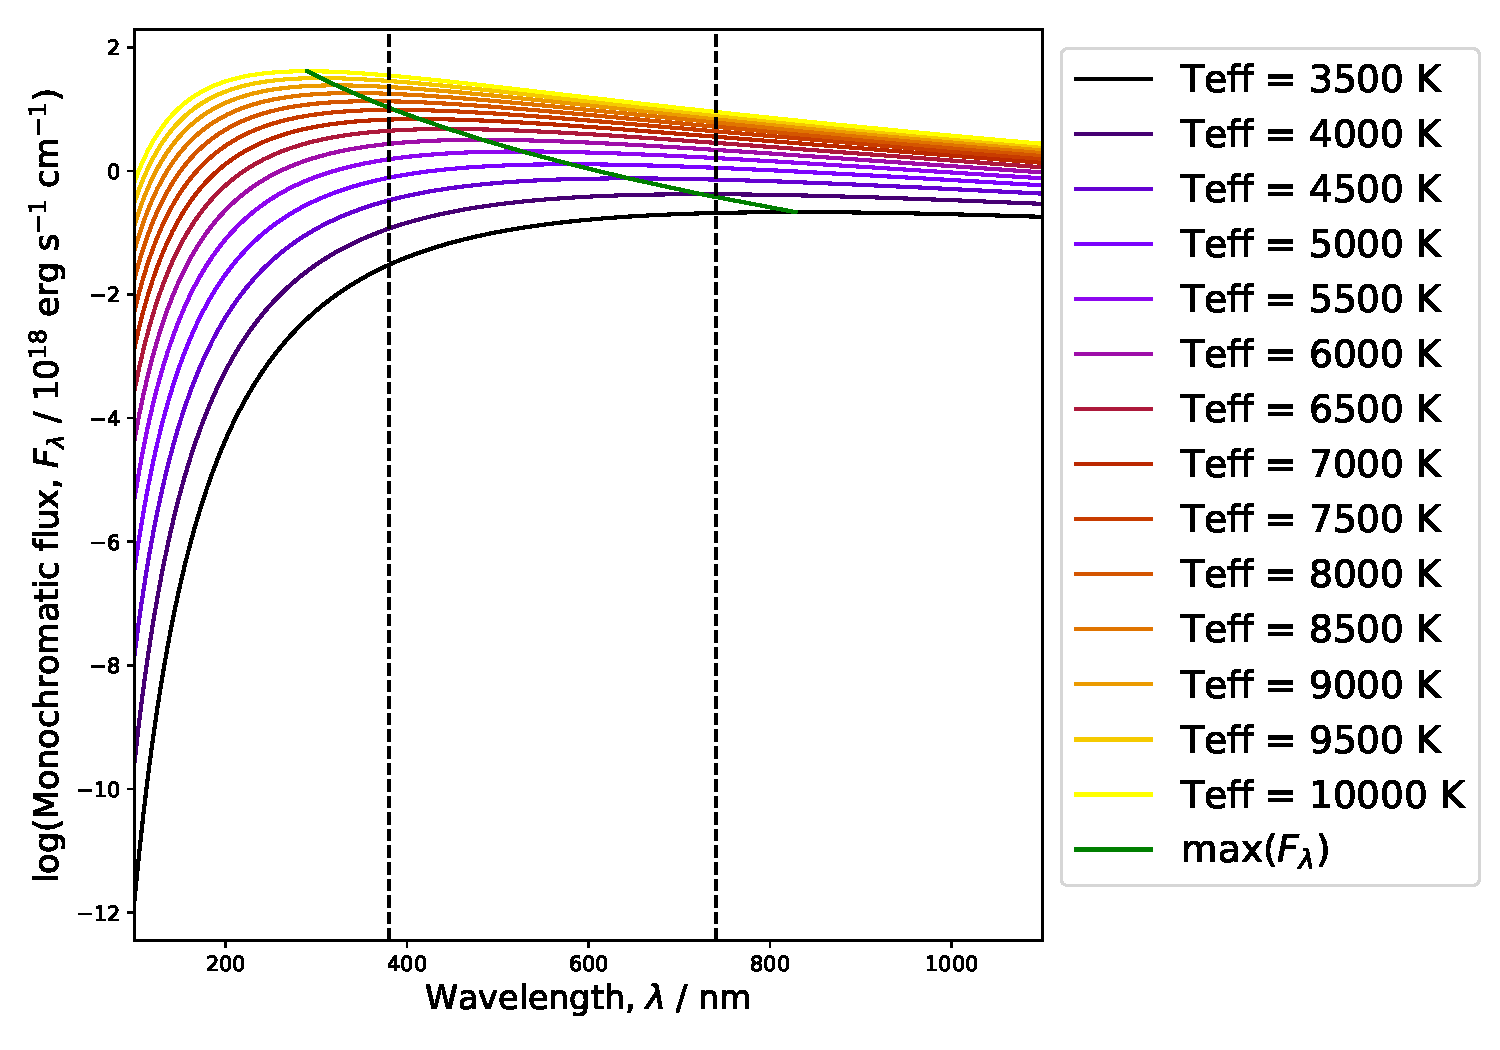
\includegraphics[width=1.0\textwidth]{blackbody_teff_logF_illustration.pdf}
\caption{Plot of the logarithm of monochromatic flux of a black body for different stellar effective temperatures, as a function of wavelength. The black dashed lines mark the approximate limits of the visible part of the EM spectrum. The green curve represents the variation of the Planck Law maxima with effective temperature.}
\label{planck_curve}
\end{center}
\end{figure}

The effective temperature ($T_{\textnormal{eff}}$) of a star is defined as the thermodynamic temperature of a black body which produces the same stellar flux across all wavelengths (known as the bolometric flux) as that produced by the star. The equation of the radiation emitted by a black body produces the body's flux per unit wavelength per unit angular viewing area, $F_{\lambda,bb}$, known as the black body's monochromatic flux. The equation, known as the Planck Law, is as follows:


\begin{equation}
F_{\lambda,bb} = \frac{2hc^{2}}{\lambda^{5}\left(\exp\left({\frac{hc}{\lambda k_{B}T}}\right) - 1\right)}
\label{planck_bb}
\end{equation} 

where $T$ is the thermodynamic temperature of the black body, $h$ is Planck's constant, $c$ is the vacuum speed of light and $k_{B}$ is Boltzmann's constant. This equation also holds if the light wave frequency is used instead of the wavelength, with the monochromatic flux $F_{\nu,bb}$ now being the black body flux per unit frequency:

\begin{equation}
F_{\nu,bb} = \frac{2h\nu^{3}}{c^{2}\left(\exp\left({\frac{h\nu}{k_{B}T}}\right) - 1\right)}
\label{planck_bb_freq}
\end{equation}

In this project, the definition of monochromatic flux for any given object will be reserved exclusively for the flux per unit wavelength, $F_{\lambda}$, with any calculations involving black body fluxes using Equation \ref{planck_bb}. \\*

The general approximation of stars to black bodies (and hence the actual stellar surface temperature to $T_{\textnormal{eff}}$) is valid because all stars have been observed to have spectra that closely resemble those of black bodies, with the notable exception of atmospheric absorption lines. The (intrinsic) luminosity of a star is used to define the effective temperature via:

\begin{equation}
L = 4 \pi R^{2} \sigma_{SB} T_{\textnormal{eff}}^{4}
\label{Teff_def}
\end{equation}

where $R$ is the (mean) stellar radius. Effective temperature has an effect on interstellar extinction due to its strong effect on the stellar luminosity and, hence, the flux, via the Planck Law in Equation \ref{planck_bb}. For a higher effective temperature, there will be more photons in the broad beam of light with wavelengths that make them likely to interact with the local ISM. \\*

Different chemical elements have different orbital configurations of atomic/ionic electron states. Each electron state absorbs and emits photons at a particular wavelength, which varies between individual states and between elements. Therefore, a greater proportion of light in a broadband beam is absorbed in a medium containing a mixture of many different elements than in a medium dominated by one or two elements. From astrophysical observations, it is clear that hydrogen is by far the most abundant element in the universe, with helium a clear-but-distant second. The metallicity of a star is defined as the fractional abundance of heavy elements, often approximated by iron (Fe) alone, relative to the star's hydrogen (H) abundance, compared to that of the Sun. The abundances are determined by the strength of the elements' characteristic atomic absorption lines in the stellar spectra.

\begin{equation}
\textnormal{[Fe/H]} = \log\left(\frac{N_{\textnormal{Fe}}}{N_{\textnormal{H}}}\right) - \log\left(\frac{N_{\textnormal{Fe},\odot}}{N_{\textnormal{H},\odot}}\right)
\label{FeH_def}
\end{equation}

For a generic atomic species $E$, $N_{E}$ represents its number density. For stellar observations, $N_{E}$ is measured at the surface. Since the output is logarithmic, a value of [Fe/H] = 0 indicates solar metallicity. An increase in metallicity would cause the corresponding absorption lines to be stronger, thus reducing the observable flux. An increased metallicity also implies an increase in abundance of sub-ferrous metals. The presence of more nuclear species, each with unique absorption line configurations, inevitably creates more observable lines, further increasing the apparent extinction in the spectral flux. The effect of this reduction in flux manifests itself as a reduction in the stellar luminosity and therefore the effective temperature when all other stellar properties (such as the mass and age) are fixed. The position of the star\\*

The definition of the stellar surface gravity $g$ is simply the value of the standard Newtonian gravitational acceleration, applied to the stellar surface (the mass is the total stellar mass, $M_{*}$, and the distance is the stellar radius, $R_{*}$):

\begin{equation}
g = \frac{GM_{*}}{R_{*}^{2}}
\label{gravity_def}
\end{equation}

A greater surface gravity, as can be inferred from Equation \ref{gravity_def}, represents a surface with a higher mass density. For stars, being self-gravitating, this infers a higher atomic number density.  \\*

%the effect of atomic number density on

The effects of surface gravity on the stellar emission spectrum arise directly from the quantum properties of the interactions between the photons and atomic electrons in the stellar atmosphere.\\*

When a particle, such as an electron, absorbs a photon, the absorption process is not instantaneous and therefore carries an uncertainty in the time taken for the process to be completed, with a corresponding uncertainty in energy due to the Heisenberg uncertainty principle. Across a large number of absorptions for the same initial electron state, the result is a spread in the energies of the absorbed photons. The associated emission line is therefore broadened by the multiple wavelengths of the photons. This is universal and referred to as ``natural broadening''.\\*

The impact of surface gravity arises via additional broadening effects upon these same absorption lines. When broadening effects are applied to an emission spectrum, such as a spectrum from a stellar surface, the result is that fewer photons pass through the surface, thereby reducing the surface flux seen by an outside observer. \\*

\subsection{Forbes effect} \label{forbes}
The Forbes effect occurs as a broadband beam of light, such as that passes through an extended partially-transparent medium, such as the Earth's atmosphere or an interstellar gas or dust cloud. It states that the greater the distance travelled by a light beam through the medium, the more penetrating the beam becomes \citep{1842RSPT..132..225F}. The physical basis for this effect is that those photons in the original beam with wavelengths that make them the most likely to be absorbed or refracted are separated from the beam earlier. Therefore, as the beam travels through the medium, its constituent photons are progressively less likely to be interact with the medium \citep{1995A&AS..109..293G}. Since a higher fraction of its photons are retained as the distance through the medium increases, the beam is more penetrating \citep{OHVRIL1999305}.\\*

This has the effect of producing a non-linear increase in extinction for one filter relative to the increase in another \citep{1995A&AS..109..293G,2008PASP..120..583G}. It should be emphasised that the Forbes effect occurs regardless of the source star's spectral type, and therefore represents an additional source of uncertainty when calculating extinction for highly-reddened stellar populations. \\*

\subsection{Determining properties of stellar populations}
\subsubsection{The role of CMDs}
If we compare the individual black body spectra in Figure \ref{planck_curve}, it can be seen that the maximum monochromatic flux of the black body occurs at an increasingly shorter wavelength for objects with increasingly higher temperatures. This makes the object appear bluer to an observer. The relationship between the wavelength at which the monochromatic flux is maximal ($\lambda_{max}$) and the black body temperature is quantified by Wien's displacement law:

\begin{equation}
\lambda_{max} T = 2.898 \times 10^{6} \textnormal{ nm K}
\label{wien_eq}
\end{equation}

More importantly, Figure \ref{planck_curve} demonstrates that, within the UV-to-IR wavelength regime, the change in monochromatic flux between values at two different wavelengths is always greater for stars with higher effective temperatures. Therefore, to measure a star's effective temperature, observers compare the star's observed flux in two filters operating at different wavelengths within this range. The difference between the star's flux magnitudes in each of the two filters is then taken, with the flux in the redder filter being deducted from that of the bluer filter. This quantity is known as the colour index. For two filters $X$ and $Y$, with $X$ being bluer than $Y$, the colour index of observations made using those filters, $(X-Y)$, is defined as:

\begin{align}
\begin{split}
(X-Y) &= m_{X} - m_{Y} \\
 &= (m_{X,0} - m_{Y,0}) + (A_{X} - A_{Y}) \\
 &= (X-Y)_{0} + E(X-Y)
\end{split}
\end{align}

where $(X-Y)_{0}$ is the true or intrinsic colour index of the object and $E(X-Y) = A_{X} - A_{Y}$ is known as the colour excess, but can also be denoted in literature using the term ``reddening''. The colour excess represents the effect of extinction on the observed colour index. Its importance arises from the prominence of the intrinsic colour index in determining effective temperature. Higher values of $(X-Y)$ indicate redder stars, with lower effective temperatures.\\*

The most commonly-used colour index, employed as a reference for most optical observations, is the Johnson ($B-V$) index \citep{1953ApJ...117..313J}. This is due to these filters being the among most widely-used and best-studied available, allowing for better comparisons of different data, including data from older archives.\\*

It can be seen from Equation \ref{Teff_def} that the luminosity (and therefore flux) of a star is dependent on radius as well as effective temperature. If a plot is made of luminosity against effective temperature (a Hertzsprung-Russell diagram), it can be seen that all stars in a given star cluster follow a single, complex track. Because the stars are approximately the same age in a typical cluster population, this track is know as an isochrone. Isochrones for different population ages and metallicities are calculated using theoretical stellar models, which cover the largest possible spread of initial stellar masses for the required age.\\*

By examining the flux-magnitude equations from both this section and Section \ref{ext_def}, it becomes clear that both the absolute filter magnitudes and the intrinsic colour indices can be used, together with bolometric corrections, to calculate the luminosity from observational data. To determine the detailed properties of stellar populations, all stars in an observational sample or star cluster are plotted together on a pair of axes known as a colour-magnitude diagram (CMD), which represents an observational analogue of the HR diagram. The absolute magnitude of stars in a given filter $Z$, $M_{Z}$, is on the y-axis, with the flux increasing (and the magnitude value decreasing) upwards. The intrinsic colour index of the stars in two filters $X$ and $Y$, $(X-Y)_{0}$, is on the x-axis, with the values increasing (and stars becoming redder) to the right. In practice, due to the unknown extinction coefficients of the individual stars and the cluster as a whole, the axial parameters  are $M_{\textnormal{ext},Z}$ and $(X-Y)$. Note that filter $Z$ may be the same as either $X$ or $Y$. \\*

In practice, the universal general shape and position of stellar populations in the HR diagram and each observational CMD, particularly the position and shape of the main sequence, provides a highly useful tool for comparing stellar populations with unknown distances and extinction coefficients to known examples and to theoretical models. This is done by alignment of the respective main sequences in CMDs, particularly the upper main sequence, which contains the most luminous MS stars and is less sensitive to the (initially unknown) value of the cluster metallicity than the lower MS. \\*

The age of an observed stellar population are determined by, firstly, correcting the data for the effects of distance and extinction and, secondly, aligning a series of isochrones, each of a different age, with the main-sequence (MS) of the observed data. The accepted age of the population is that of the isochrone which most closely follows the progression of stars along the main-sequence turn-off (MSTO). As such, any errors in the estimated extinction can potentially change the age of the best-fit isochrone and therefore produce an erroneous estimate of the true population age.

\subsubsection{Comparing theoretical and observational quantities}
For any observational dataset of stars, the stars' individual extinction values will be completely unknown from the data alone. In order to compare observational and theoretical data, the most convenient approach is to add the (theoretical) extinction value(s) to the theoretical dataset magnitudes (i.e., absolute magnitudes), before comparing to the distance-corrected observational data. As a result, the quantity from each dataset that is being compared is the absolute magnitude plus the extinction coefficient in each filter. If we label this quantity $M_{\textnormal{ext},X}$ for a generic filter $X$, we can define it as:

\begin{equation}
M_{\textnormal{ext},X} = M_{X} + A_{X}
\label{MextX_def}
\end{equation}

Using Equations \ref{extinc_X} and \ref{DM_X}, Equation \ref{MextX_def} can now be rewritten such that $M_{\textnormal{ext},X}$ is defined using both quantities derived directly from observations and those determined by theoretical models:

\begin{align}
\begin{split}
M_{\textnormal{ext},X} &= M_{X} + A_{X} \textnormal{ (theoretical data)}\\
 &= m_{X} + 5 - 5\log\left(\frac{d}{\textnormal{pc}}\right) \textnormal{ (observational data)}
\end{split}
\label{MextX_eq}
\end{align}

This allows for direct comparison of theoretical data, whose stars are treated with theoretically-determined $A_{X}$ values, with distance-corrected observational data, whose stars have unknown $A_{X}$ values. Therefore, this provides a pathway for comparing the standard treatment of extinction (constant $A_{X}/A_{V}$ ratios) with the treatment proposed in this project ($A_{X}/A_{V}$ varying as functions of intrinsic stellar parameters). \\*

\subsection{Empirical extinction curves} \label{empirical}

\begin{figure}[h]
\begin{center}
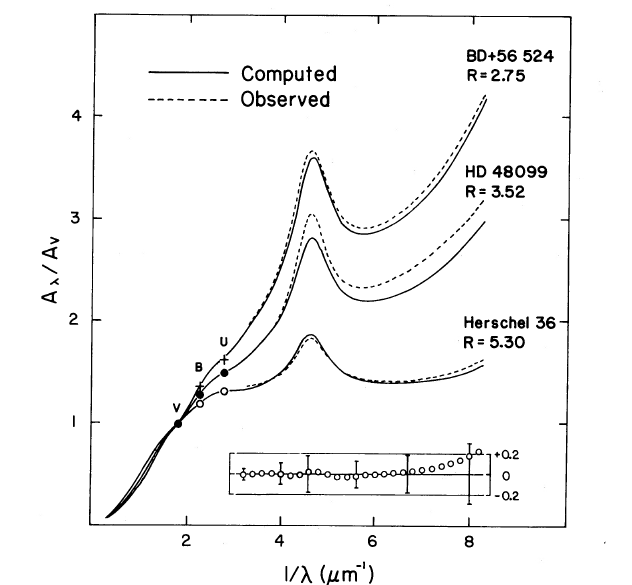
\includegraphics[width=1.0\textwidth]{cardelli_curve_fig4_crop.png}
\caption{Variation of the extinction, normalised to the $V$-band extinction $A_{V}$, as a function of wavelength, in spectral regions ranging from the IR (left) to the UV (right). The solid lines are calculated using Equation \ref{CCM_general} at the given $R_{V}$ values. These values represent the lines of sight for their respective source stars, which are listed alongside.  Source: \cite{1989ApJ...345..245C}}
\label{cardelli_curve}
\end{center}
\end{figure}

\cite{1985ApJ...288..618R} found that outside dense molecular clouds, which have high opacities and whose lines-of-sight are less frequently used as a result, all extinction laws for all Johnson filters studied were uniform between wavelengths of 1 and 13 $\mu$m when observing sources in the direction of the Galactic Centre. This result was then used to produce constant $A_{X}/A_{V}$ extinction ratios in the same filters. They also determined the now-widely used global average value of 3.08 (~3.1) for $R_{V} = A{V}/E(B-V)$, known as the total-to-selective extinction ratio,  for the diffuse ISM. \\*

\cite{1989ApJ...345..245C} used observations of mostly O- and B-type main-sequence stars to produce empirical equations describing the mean ratio of extinction coefficients at a specific wavelength $\lambda$ ($A_{\lambda}$) to the extinction in the Johnson-$V$ filter ($A_{V}$), respectively. From this point onward, this ratio will be referred to as $A_{\lambda}/A_{V}$. They produced a basic equation of the form:

\begin{equation}
A_{\lambda}/A_{V} = a(x) + b(x)/R_{V},
\label{CCM_general}
\end{equation}

where $x \equiv 1/\lambda$ and $R_{V} \equiv A(V)/E(B-V)$. The significance of $R_{V}$, as noted in the same paper, comes from its usefulness as an indicator of the nature of the interstellar medium through which the observed light travels in order to reach the observer. The total wavelength range was divided into 4 sub-ranges, each with a governing pair of empirically-determined equations to calculate $a(x)$ and $b(x)$, respectively. The resulting extinction-ratio profiles for three lines of sight are displayed in Figure \ref{cardelli_curve}. This model underpins more recent studies of intrinsic effects on extinction \citep{2008PASP..120..583G,2018MNRAS.479L.102C}, and provides the basis for the synthetic $A_{X}/A_{V}$ datasets in this project. Equation \ref{CCM_general} has become a standard model for theoretical studies to employ for predictions made in the UV, optical and near-IR wavelength regions, although it is not always accurate \citep{1994ApJ...422..158O,1999PASP..111...63F}. \\*

\cite{1994ApJ...422..158O} found deviations from the \cite{1985ApJ...288..618R} extinction law in the soft-UV spectral range using a sub-sample of 22 stars from the same dataset. This was attributed to the uncertainty in the short-wavelength cutoff of the UV-range Johnson $U$ filter and to the presence of the Balmer discontinuity within the limits of the filter bandpass.\\*

\cite{1999PASP..111...63F} found that, due to the broadband nature of the Johnson filters and the general decrease of extinction with wavelength, the \cite{1989ApJ...345..245C} relations overestimate the extinction in the near-IR and blue-visible Johnson filters. The study put forward corrections to the equations for $a(x)$ and $b(x)$ for these wavelength regions. However, in the UV region covered by  the \cite{1989ApJ...345..245C} equations, the equations are accurate for 93\% of a homogeneous UV observational database \citep{2004ApJ...616..912V}.\\*

\cite{2008PASP..120..583G} produced data tables of $A_{X}/A_{V}$ for stellar atmosphere models with parameters $T_{\textnormal{eff}}$, log($g$) and [Fe/H]. They carried this out using the same ATLAS9 data \citep{2004astro.ph..5087C} that was used to generate the data for this project, but also combined it with data from other studies \cite{2002A&A...391..195G}, resulting in data covering a parameter space extending beyond the ATLAS9 limits in all three parameters. They used the data tables to calculate the $A_{X}/A_{V}$ values for the stellar models in Padova theoretical isochrones. While determining that the values of $A_{X}/A_{V}$ varied significantly with $T_{\textnormal{eff}}$ and log($g$), the variation with metallicity was found to be ~0.17$\%$ between [Fe/H] = 0.0 and [Fe/H] = -2.5. They found that, when they set $A_{V} = 6$, there was a systematic shift for the ACS system between extinction values calculated star-wise using the tables of $A_{X}/A_{V}$ data and a constant extinction value. The constant values of $A_{X}/A_{V}$ were calculated from a yellow dwarf in the low-extinction regime. Overall, the $A_{X}/A_{V}$ tables produced a smaller extinction coefficient in the F814W filter and a larger (F475W-F814W) colour index value. It also caused a change in the shape of the curve at the MSTO. They then applied the data from the tables to the case of the globular cluster M92. They found the optimal metallicity to be $Z = 0.0004$ ([Fe/H] $\approx$ -1.6) instead of the value obtain by previous observers of $Z = 0.0001$ ([Fe/H] $\approx$ -2.2). Therefore, their use of $A_{X}/A_{V}$ data caused the estimated cluster metallicity to be greater than when using the standard one-size-fits-all approach to extinction.\\*

Casagrande \& Vandenberg (2014, 2018a, 2018b) created simple  models for the parameter $R_{X}  = \frac{A_{X}}{E(B-V)}$, consisting of a quadratic variation with effective temperature and a linear variation with metallicity (they found no significant variations with surface gravity) in multiple telescope filter systems. This was based on MARCS model stellar atmospheres, which have an upper $T_{\textnormal{eff}}$ limit of 8000K \citep{2008A&A...486..951G}. The equation is independent of surface gravity and has the following form:

\begin{equation}
R_{X} = a_{0} + T_{4}(a_{1} + a_{2}T_{4}) + a_{3}\textnormal{[Fe/H]}
\label{casagrande_ext_fit}
\end{equation}

where $T_{4} = 10^{-4} \times T_{\textnormal{eff}}$. The equation is valid for $5250\textnormal{K} \leq T_{\textnormal{eff}} \leq 7000\textnormal{K}$. Although these models are mathematically simple (with only 4 coefficients), the limited $T_{\textnormal{eff}}$ range in which they are applicable is problematic, particularly in the red giant branch (RGB) and lower main sequence of any stellar population.\\*

\section{The standard treatment of extinction in observed stellar populations} \label{standard_ext}

In observations, the extinction for a given source is initially unknown. For a stellar population, observers must make use distinctive features of stellar populations that can be used as standard candles to estimate distance moduli to the population (see Equation \ref{distance_modulus}).

The treatment of extinction in observational surveys is usually via a constant value for the ratio of extinction in a given filter $X$, denoted by $A_{X}$, divided by the extinction in the well-studied Johnson-$V$ filter, $A_{V}$. The value used for this ratio, denoted by $A_{X}/A_{V}$, is often taken from \cite{1985ApJ...288..618R}. This approach has the significant issue of producing $A_{X}/A_{V}$ values that do not account for  variations in the monochromatic flux between stars with different physical parameter values when integrated over the filter's wavelength range, which can be several orders of magnitude. As shown in Figure \ref{planck_curve}, the monochromatic flux at a given wavelength varies greatly with effective temperature, as does the ratio between monochromatic fluxes of stars of different temperatures. This makes the notion that stars of different temperatures lose the same flux in a given filter passband, which is implied by the use constant extinction ratios across all stellar classes, inherently flawed. Stars with higher effective temperatures have emission spectra with much higher and (proportionally greater) fluxes at the shorter wavelengths which are most impacted by interstellar extinction. Therefore, it should be expected that hotter stars experience higher extinctions $A_{X}$ for a given filter, not equal values.\\*

\cite{2017Galax...5...28O} used the tabulated extinction ratio tables resulting from \cite{2008PASP..120..583G}, which demonstrated the significant effect of stellar parameters on the calculated extinction ratios, to search for potential discrepancies in the predicted ages of isochrones after the addition of extinction. This was performed for isochrones with real ages between 12 and 13 Gyr and employed a small selection of Johnson ($B$,$V$ and $I$) and ACS (F606W, F775W and F814W) broadband filters. They found that, once the assumption of uniform extinction across the entire population was removed by employing the \cite{2008PASP..120..583G} data, the isochrone position in the CMD shifted such that, at $A_{V} = 1$, the MSTO of a 12 Gyr isochrone with individual stellar extinction values added is the same as the position of a 12.5 Gyr isochrone with the standard single extinction value added.\\*

\section{Project objective}
This project will study the variations of the extinction ratios $A_{X}/A_{V}$ in multiple photometric filters within multiple filter systems with changes in $T_{\textnormal{eff}}$, $g$ and [Fe/H]. This will be carried out across as large a range of stellar types as possible.\\*

Furthermore, this project will attempt to use mathematical functions as models to describe these variations in $A_{X}/A_{V}$. The ultimate goal is to use this simplification of the variations to determine the differences in the estimated optimal ages, elemental abundances (i.e., metallicity) and extinction reference values of stellar populations between simulating extinction using values calculated for each star and using a single value for extinction across the entire population, which is the current standard method. If such differences exist and if they are of significant size, it could cause a recalculation of the properties of observed star clusters. This could potentially cause a reinterpretation of these clusters' history, including where and when they formed in the Milky Way and the chemical enrichment of the gas that formed their stars. \\*



\chapter{Methodology}
\section{Calculating extinction ratio data}
When observing stars through a photometric filter, only a small fraction of the bolometric stellar flux that reaches the telescope is detected, as can be seen from the filter response functions in Figures \ref{Gaia_response_funcs}-\ref{ACS_response_funcs}. The missing spectral information resulting from this observational constraint renders it difficult to determine the stellar properties, including interstellar extinction. This must be mitigated before an accurate value of the extinction coefficient can be determined. The mitigation is carried out by calculating bolometric corrections.\\*

The use of bolometric corrections requires the detailed knowledge of stellar spectra least susceptible to significant extinction, meaning, in effect, nearby stars. Only with complete knowledge of the spectrum from a reference star can the true spectrum of a distant star with unknown extinction be calculated. The spectra of these stars can be computed by using a grid of predicted fluxes from a stellar atmosphere model, the grid being composed of the stellar parameters known to change emission in stellar atmospheres. These are effective temperature, surface gravity and metallicity. For all filter systems studied in this project, the nearby bright star Vega ($\alpha$ Lyr) was used as the reference object. Using Vega as the reference star is the most well-known approach to photometric calibration \citep{2014MNRAS.444..392C}.\\*

After accounting for the effect of interstellar extinction on an object's emission, its apparent magnitude in the wavelength range of a given filter $X$, defined as increasing from the shortest ($\lambda_{1}$) to the longest ($\lambda_{2}$) wavelength for which its response function is non-zero, can be calculated as:

\begin{equation}
m_{X} = -2.5 \log_{10} \left(\frac{ \int_{\lambda_{1}}^{\lambda_{2}} f_{\lambda} \left( 10^{-0.4 A_{X,\lambda}} \right) S_{\lambda} d\lambda }{ \int_{\lambda_{1}}^{\lambda_{2}} f_{\lambda}^{0} S_{\lambda} d\lambda }\right) + m_{X}^{0}
\label{app_mag_def}
\end{equation}

where $f_{\lambda}$ represents the (theoretical) monochromatic flux at a given wavelength $\lambda$ at the observer distance from the source, $A_{X,\lambda}$ is the extinction coefficient in $X$ as a function of wavelength and $S_{\lambda}$ represents the filter response function of $X$. $f_{\lambda}^{0}$ and $m_{X}^{0}$ represent the monochromatic flux and apparent magnitude, respectively, in $X$of a known reference object, which is Vega in the case of this project.

%Since our goal, ultimately, is to document potential effects of fundamental stellar properties upon observables, we need to connect the observational and idealised scenarios, for which we use bolometric corrections.

To derive the equation linking a bolometric correction with the extinction parameter, we start with the definition of a bolometric correction in a filter $X$, which is denoted by $BC_{X}$:

\begin{equation}
BC_{X} \equiv M_{\textnormal{bol}} - M_{X}
\label{BC_def}
\end{equation}

where $M_{X}$ is the absolute magnitude of the object in $X$ and $M_{\textnormal{bol}}$ is its (predicted) absolute bolometric magnitude, defined relative to the Sun using:

\begin{equation}
M_{\textnormal{bol}} = M_{\textnormal{bol},\odot} - 2.5 \log_{10} \left( \frac{4\pi R^{2}F_{\textnormal{bol}}}{L_{\odot}} \right)
\label{mbol_sun}
\end{equation}

where  $F_{\textnormal{bol}}$ is the bolometric stellar flux at its surface, $R$ is the stellar radius, $M_{\textnormal{bol},\odot}$ is the solar absolute bolometric magnitude, which is assumed in this work to have a value of 4.75 and $L_{\odot}$ is the solar luminosity, for which a value of $3.844 \times 10^{33}$ erg s$^{-1}$ is used. Bolometric corrections can be expressed as a function of extinction using the definition of $M_{X}$ in terms of $m_{X}$ and the distance $d$ to the source:

\begin{equation}
M_{X} = m_{X} - 2.5 \log_{10}\left( \left( \frac{d}{10 \textnormal{pc}} \right)^{2} \right),
\label{abs_mag_def}
\end{equation}

together with the equation $f_{\lambda}d^{2}=F_{\lambda}R^{2}$, where $F_{\lambda}$ is the monochromatic flux at $\lambda$ at the stellar surface. This gives the final function for a bolometric correction for filter $X$:

\begin{align}
\begin{split}
BC_{X} &= M_{\textnormal{bol},\odot} - m_{X}^{0} - 2.5 \log_{10} \left( \frac{4\pi R^{2}F_{\textnormal{bol}}}{L_{\odot}} \right) \\
&+ 2.5 \log_{10} \left( \frac{\int_{\lambda_{1}}^{\lambda_{2}} F_{\lambda} \left( 10^{-0.4 A_{X,\lambda}} \right) S_{\lambda} d\lambda}{\int_{\lambda_{1}}^{\lambda_{2}} f_{\lambda}^{0} S_{\lambda} d\lambda} \right)
\label{BC_extinc}
\end{split}
\end{align}

For a filter $X$, the extinction parameter $A_{X} = A_{X,\lambda}$ is usually parametrised relative to the extinction in the well-studied Johnson-$V$ filter, $A_{V}$. To extract $A_{X}$, we use the simple relation:

\begin{equation}
A_{X,\lambda} = \left( \frac{A_{X,\lambda}}{A_{V}} \right) A_{V}
\label{ratio_eq}
\end{equation}

together with the chosen value of $A_{V}$ (for this project the values were $A_{V} = 0$, 1 - note that $BC_{X}(A_{V}=0)$ essentially assumes no extinction in any filter), before taking the difference between the two $BC_{X}(A_{V})$ outputs, giving the following equation \citep{2008PASP..120..583G}:

\begin{align}
\begin{split}
BC_{X}(0) - BC_{X}(A_{V}) &= \left(A_{X}/A_{V}\right)A_{V}
\label{BCs_diff}
\end{split}
\end{align}
%\\ &\approx \left(A_{X}/A_{V}\right)A_{V}

As demonstrated in the equation above, any dependence of the $A_{X}/A_{V}$ data on the Vega measurements or (as yet unknown or uncertain) bolometric quantities from Equation \ref{BC_extinc} is eliminated during the subtraction. \\*

****
The Forbes effect has an impact on the non-zero $A_{V}$ value used in Equation \ref{BCs_diff} because if a uniform medium is assumed, as here, where $R_{V}$ is held constant at the standard diffuse ISM value of 3.1 \citep{1989ApJ...345..245C}, a larger $A_{V}$ value implies a longer path through the ISM, and thus a stronger Forbes effect. According to \cite{2008PASP..120..583G}, any significant impact from the Forbes effect on the values of $A_{X}/A_{V}$ occurs for a chosen $A_{V} \gtrsim 4$. They found that the effect was particularly strong for stars with $T_{\textnormal{eff}} \lesssim 3000$K and that, unsurprising, it became greater as the wavelength range covered by the filter response function increased.\\*
****

Once the $A_{X}/A_{V}$ data was calculated, functions of the three stellar parameters described in Section \ref{params} were created and fitted to the data, with the function coefficients acting as the free parameters to be fitted. The best-fit values of these coefficients were calculated using a least-squares fit algorithm.\\*

\section{Software used}
To generate the predicted stellar flux, pre-calculated ATLAS9 model stellar atmosphere \citep{1993KurCD..13.....K} tables of monochromatic fluxes were produced. These tables incorporated wavelengths ranging from 9 nm to 160,000 nm, with a resolution of 2 nm or less in the UV. Table 1 of \cite{2004astro.ph..5087C} contains precise details of the coverage of the model atmospheres in ($T_{\textnormal{eff}}$, log($g$)) parameter space, while a brief summary  of the limits of the space is listed in Table \ref{atlas9_input}. Four input metallicities were used for ATLAS9, at values of [Fe/H] = -2, -1, 0 and 0.5, covering the metallicities of most observed globular and open clusters. Each metallicity case was subject to the same coverage in ATLAS9. As shown in Figure \ref{Teff-logg coverage}, with the exception of the coolest, and therefore faintest, main sequence stars in the bottom right of the figure, the ATLAS9 grid covers the required parameter space for isochrones of all ages. The variation of isochrones at the plotted ages with metallicity is not significant with respect to the grid coverage. \\*

\begin{figure}[h]
\begin{center}
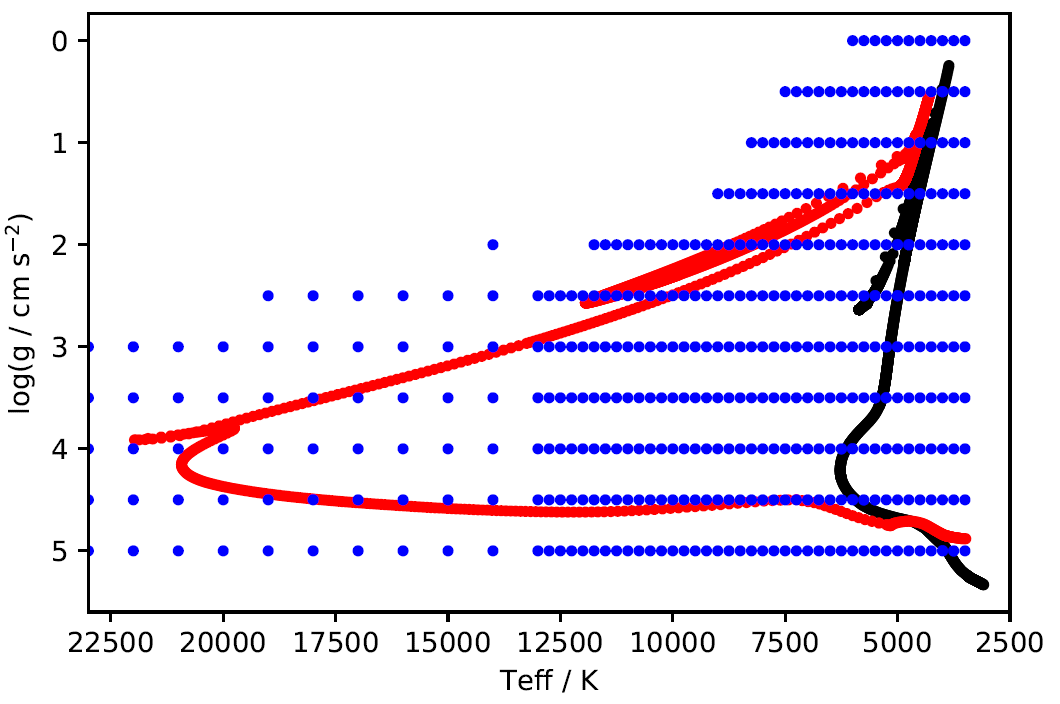
\includegraphics[width=1.0\textwidth]{ATLAS9_grid_BaSTI_coverage_2ages_crop.png}
\caption{$T_{\textnormal{eff}}$-log($g$) scatter plot for a BaSTI 50 Myr, [Fe/H] = -1 isochrone (red), a BaSTI 12 Gyr, [Fe/H] = -1 isochrone (black) and ATLAS9 model grid (blue) for $T_{\textnormal{eff}} \leq 23000$ K.}
\label{Teff-logg coverage}
\end{center}
\end{figure}

The tables of bolometric corrections were generated using a FORTRAN 77 code which incorporated Equations \ref{BC_def}-\ref{BCs_diff} and input data files with tables describing the response functions of all relevant filter systems (described in detail in Section \ref{filter_desc}) at the same wavelengths as those listed in the ATLAS9 model atmosphere tables, with the number of tables for each stellar metallicity value equal to the total number of ($T_{\textnormal{eff}}$, log($g$)) combinations available.\\*

Once the bolometric correction tables were produced, all subsequent processes were written in Python 2.7 in the form of an IPython notebook. The repository containing all data, plots and programme codes for this project can be found at \protect\url{https://github.com/AlexlwAstro/phd_work}.\\*


\begin{table}
\begin{center}
\begin{tabular}{cccc}
\hline
Parameter / unit & Minimum & Maximum & Number of values \\
\hline
$T_{\textnormal{eff}}$ / K & 3500 & 50000 & 76 \\
log( $g$ / cm s$^{-2}$) & 0.0 & 5.0 & 11 \\
$\textnormal{[Fe/H]}$ & -2.0 & 0.5 & 4 \\
\hline
\end{tabular}
\caption{Ranges for the input parameters for ATLAS9 atmospheric models}
\label{atlas9_input}
\end{center}
\end{table}

The isochrones used were generated using the latest Bag of Stellar Tracks and Isochrones (BaSTI) web interface (\cite{2004ApJ...612..168P}, \cite{2018ApJ...856..125H}). The filter systems whose throughput data were employed by BaSTI to generate the fluxes for the isochrones were ACS, WFC3 and Gaia-DR2. It should be noted that the WFC3 isochrone output for BaSTI does not include flux magnitudes for the F300X filter.\\*

\section{Filters studied} \label{filter_desc}
In this project, three broad-band filter systems were employed. Two are systems on board the Hubble Space Telescope (HST). These are the Advanced Camera for Surveys (ACS), installed in 2002 on the HST \citep{2007AJ....133.1658S}, and the Ultraviolet Imaging Spectrograph channel of the Wide-Field Camera 3 (WFC3/UVIS), installed on the HST in 2009 \citep{2010wfc..rept...14K,2010SPIE.7731E..0ZM}). The third is the single set of three broadband filters mounted on the Gaia space observatory  \citep{2010A&A...523A..48J}, launched in 2013. \\*

Reference will also be made to the Johnson-Morgan filter system (often simply known as the Johnson system) UBV \cite{1953ApJ...117..313J}, later extended as the Johnson-Cousins UBVRI \cite{1990PASP..102.1181B} system, which has been in use for decades and continues to be be the standard reference for more modern filter systems. Of particular importance are the Johnson blue ($B$) and yellow ($V$) filters, as these formed the original benchmark for observing stellar populations and evolutionary stages. \\*

\begin{figure}[h!]
\begin{center}
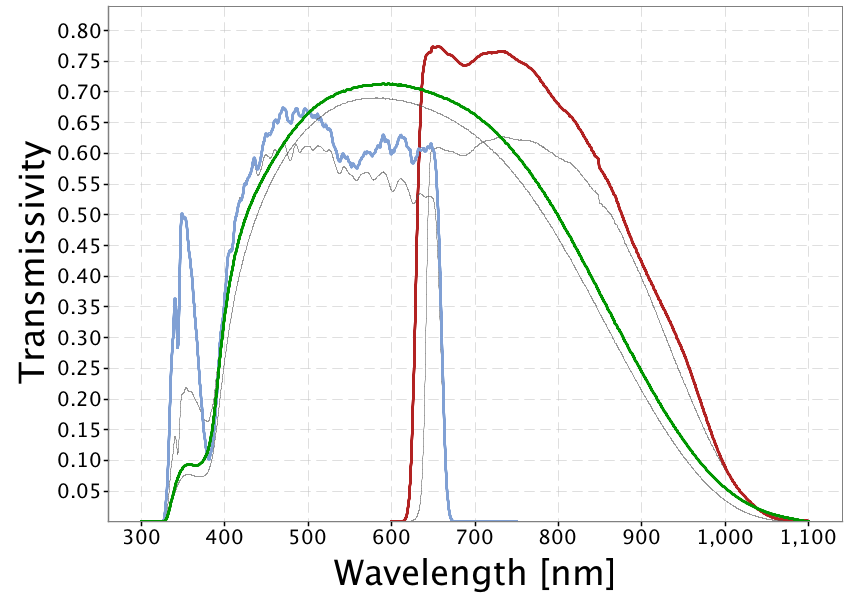
\includegraphics[width=1.0\textwidth]{GaiaDR2Passbands.png}
\caption{Filter response functions for Gaia photometric filters. Source: \protect\url{https://www.cosmos.esa.int/web/gaia/iow_20180316}}
\label{Gaia_response_funcs}
\end{center}
\end{figure}

\begin{figure}[h]
\begin{center}
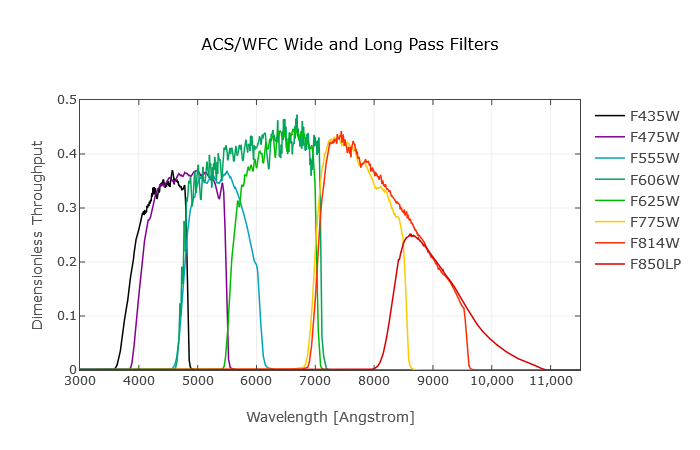
\includegraphics[width=1.0\textwidth]{ACS_Wide.png}
\caption{Filter response functions for wide-field ACS filters. Source: \protect\url{http://www.stsci.edu/hst/acs/analysis/throughputs}}
\label{ACS_response_funcs}
\end{center}
\end{figure}

\begin{figure}[h!]
\begin{center}
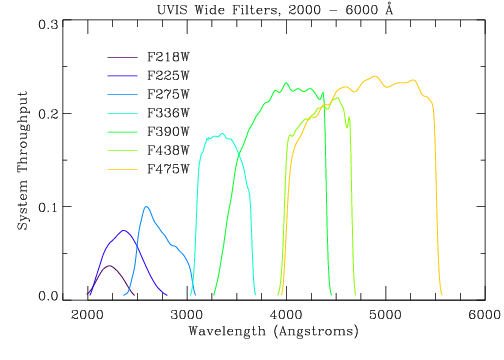
\includegraphics[width=1.0\textwidth]{UVIS_Wide1.jpg}
\caption{Filter response functions for wide-field WFC3 filters. Source: \protect\url{http://www.stsci.edu/hst/wfc3/ins_performance/throughputs/UVIS_filterthru.html}}
\label{WFC3_response_funcs1}
\end{center}
\end{figure}

\begin{figure}[h]
\begin{center}
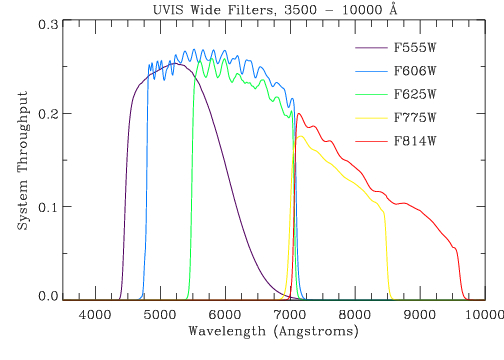
\includegraphics[width=1.0\textwidth]{UVIS_Wide2.jpg}
\caption{Filter response functions for wide-field WFC3 filters. Source: \protect\url{http://www.stsci.edu/hst/wfc3/ins_performance/throughputs/UVIS_filterthru.html}}
\label{WFC3_response_funcs2}
\end{center}
\end{figure}

The standard treatment of extinction is to apply a single constant value of the extinction ratio for a given filter $X$. This quantity is usually expressed as a fixed extinction ratio $A_{X}/A_{V}$ of the (constant) coefficient value in the Johnson-$V$ filter, the standard visual comparison filter. This value is maintained for all stars, regardless of the different effective temperatures, metallicities or surface gravities of the different types of stars present in any given population. The wavelengths of optical light lie between 3800 \AA and 7400 \AA, with the $V$ filter having a central wavelength of 5500 \AA.

\begin{table}
\begin{center}
\begin{tabular}{cccccc}
\hline
System & Filter & $\lambda_{\textnormal{cen}}$ / \AA & FWHM / \AA & $\lambda_{\textnormal{min}}$ / \AA & $\lambda_{\textnormal{max}}$ / \AA \\
\hline
% results: previously listed & from source website specified in caption					added more info: l_min & l_max
& F435W & 4359 & 881 & 3610 & 4860 \\ % & 4760 & 729
& F475W & 4781 & 1403 & 3863 & 5563 \\ % & 5000 & 986
& F555W & 5413 & 1236 & 4584 & 6209 \\ % & 5060 & 841
ACS & F606W & 5961 & 2255 & 4634 & 7180 \\ % & 6690 & 1566
& F625W & 6323 & 1390 & 5446 & 7100 \\ % & 6480 & 978
& F775W & 7763 & 1517 & 6804 & 8632 \\ % & 7320 & 1017
& F814W & 8117 & 2096 & 6885 & 9648 \\ % & 7460 & 1657
\hline
& F218W & 2216 & 329 & 1990 & 2603 \\ % & 2175 & 300
& F225W & 2341 & 464 & 1990 & 2968 \\ % & 2250 & 500
& F275W & 2696 & 417 & 2282 & 3119 \\ % & 2750 & 500
& F300X & 2722 & 660 & 2137 & 4098 \\ % &  & 2775
& F336W & 3368 & 550 & 3014 & 3707 \\ % & 3375 & 550
& F390W & 3929 & 951 & 3255 & 4470 \\ % & 3900 & 1000
WFC3 & F438W & 4322 & 674 & 3895 & 4710 \\ % & 4320 & 695
& F475W & 4768 & 1482 & 3942 & 5582 \\ % & 4750 & 1520
& F555W & 5262 & 1578 & 4381 & 7045 \\ % & 5410 & 1605
& F606W & 5941 & 2298 & 4700 & 7204 \\ % & 5956 & 2340
& F625W & 6274 & 1573 & 5414 & 7138 \\ % & 6250 & 1550
& F775W & 7725 & 1454 & 6869 & 8571 \\ % & 7760 & 1470
& F814W & 7814 & 1505 & 6978 & 9684 \\ % & 8353 & 2555
\hline
& $G$ & 6631 & 4397 & 3321 & 10515 \\ % & 6730 & 4400
Gaia & $G_{\textnormal{bp}}$ & 5330 & 2530 & 3283 & 6714 \\ % & 5320 & 2530
& $G_{\textnormal{rp}}$ & 7896 & 2956 & 6296 & 10637 \\ % & 7970 & 2960
\hline

\end{tabular}
\caption{Basic properties of the filters employed in this project. See text for details. Source: \protect\url{http://svo2.cab.inta-csic.es/svo/theory/fps3/index.php}}
\label{filter_basics}
\end{center}
\end{table}

In Table \ref{filter_basics}, all the filters used for this project are listed. The name of each filter is displayed alongside its central wavelength ($\lambda_{\textnormal{cen}}$), full-width at half-maximum (FWHM) and the minimum ($\lambda_{\textnormal{min}}$) and maximum ($\lambda_{\textnormal{max}}$) detection wavelengths. Hence, when combined, these filters cover wavelengths from the soft-ultraviolet (soft-UV) to the near-infrared (NIR), including all visible wavelengths. The FWHM is defined as the difference between the lowest and highest wavelength values at which the transmittance value is half of its maximum value for the filter, typically assuming the response function can be approximated as a Gaussian distribution centred on the central wavelength. The FWHM acts as an approximate measure of the wavelength range within which the filter can be used for observations.\\*

\section{Isochrone data fitting} \label{isoc_fit}
To obtain isochrones from the BaSTI online database, the desired age range, initial metallicity and filter system must be specified. Therefore, the values of these quantities are shared by all stellar objects. The output from the BaSTI database for each model stellar object gives the model's initial mass and current mass (i.e. after a time equal to the isochrone age), together with the logarithms of the stellar luminosity in solar units ($\log(L/L_{\odot})$) and of the effective temperature in K ($\log(T_{\textnormal{eff}})$), followed by the absolute magnitudes (with zero extinction) of the object in each filter of the system. To derive the surface gravity $g$, we must combine Equation \ref{Teff_def}, to derive the stellar radius, and Equation \ref{gravity_def}. Equation \ref{gravity_LT_calc} shows the resultant definition of $g$:

\begin{equation}
\label{gravity_LT_calc}
g = \frac{4 \pi G M_{*} \sigma_{\textnormal{SB}} T_{\textnormal{eff}}^{4}}{L_{*}}
\end{equation}

After this had been completed, each object had a co-ordinate in ($T_{\textnormal{eff}}$, log($g$)) parameter space, plus the metallicity of the overall isochrone model. To match the quantities of observational datasets (with unknown extinction) and isochrones, it is necessary to correct the observational data for distance and add extinction to the isochrones. This is that standard procedure used when analysing observational data. Thus, the $M_{\textnormal{ext},X}$ values for the isochrones and the observational data are being compared. The functions described in Section \ref{ext_models} were then applied to the dataset of stellar objects, producing values of $M_{\textnormal{ext},X}$ for each filter for all objects, as is the standard for analysing observational data with unknown extinction coefficients.

\begin{table}
\begin{center}
\begin{tabular}{ccccc}
\hline
Isochrone & $T_{\textnormal{eff}}$ & $T_{\textnormal{eff}}$ & $\log(g)$ & $\log(g)$ \\
(Age/Myr , [Fe/H]) & minimum & maximum & minimum & maximum \\
\hline
500,0.002 & 2870 & 9640 & 0.886 & 5.137 \\
1000,0.002 & 2824 & 8035 & 1.608 & 5.184 \\
5000,-1.049 & 3118 & 7112 & 0.456 & 5.318 \\
10000,-1.049 & 3086 & 6412 & 0.286 & 5.332 \\
\hline
\end{tabular}
\caption{Ranges of effective temperature and surface gravities in selected BaSTI isochrones}
\label{variable_ranges}
\end{center}
\end{table}

When comparing the two approaches to extinction, in order to test for any differences in projected isochrone age via the MSTO, a range of ages must be considered. A ``primary'' age was utilised as the true cluster isochrone age. This primary isochrone was subjected to both the function-based (FBER) and standard (fixed) extinction-ratio approaches. Two isochrones with ages equidistant from the primary were subjected to the standard approach only. All four of the resulting $M_{\textnormal{ext},X}$ isochrones were plotted together in the four chosen CMD axes, together with the original (zero-extinction) isochrone for visual reference.\\*

This procedure was employed for two values of $A_{X}/A_{V}$ for the standard (fixed) extinction treatment. Both were extracted from the ATLAS9 data tables for a log($g$) value of 5.0 to represent a main-sequence star, highly desirable when comparing MSTO positions. Given the large number of filters studied in this project, four commonly-used CMD axes were selected to test for any effects of a $A_{X}/A_{V}$ function. Two of these are specific to the WFC3 system, with one CMD each for ACS and Gaia.\\*

\section{Observational test case: NGC 6793}
To test the effects of the two different treatments of $A_{X}/A_{V}$ on observational data, both were employed to predict the isochrone parameters (age,[Fe/H] and $A_{V}$) for the open cluster NGC 6793.

NGC 6793 has little information available in the literature when compared to open clusters. Two observational studies have been published which give estimates for the properties of the cluster. Both sets of results are listed in Table \ref{NGC6793_obs}. However, it has the significant advantage of having both a very high $A_{V}$ extinction value among star clusters and a full set of Gaia parallax measurements for its member stars. The accurate distances to all its members allows for a higher degree of confidence in the position of the observed cluster CMD. Meanwhile, a high $A_{V}$ value increases any disagreement between the extinction treatments being compared for the cluster. Consequently, any resulting disagreement in estimates of the best-fit isochrone parameters for the cluster become greater and more significant. \\*

\begin{table}
\begin{center}
\begin{tabular}{ccc}
\hline
Cluster property & K05 & GC18 \\
\hline
Distance modulus / mag & 10.73 & 8.894 \\
-> distance / pc & 1400 & 601 \\
log(age / yr) & 8.64 & 8.78 \\
-> Age / Myr & 437 & 603 \\
$E(B-V)$ / mag & 0.17 & 0.272 \\
-> $A_{V}$ / mag (if $R_{V} = 3.1$) & 0.53 & 0.843 \\
$\textnormal{[Fe/H]}$ & ? & ? \\
Members & ? (> 3 ACSS-2.5) & 465 (271 with Gaia photometry) \\
\hline
\end{tabular}
\caption{Observational parameters for NGC 6793, according to \cite{2005A&A...438.1163K} (WEBDA archive page) and \cite{2018A&A...616A..10G}}
\label{NGC6793_obs}
\end{center}
\end{table}

The Gaia DR2 dataset for NGC 6793, containing the parallaxes and apparent magnitudes (in all three Gaia filters) for 338 objects identified as belonging to the cluster, was obtained. The number of objects is greater than the 271 photometric Gaia objects found by \cite{2018A&A...616A..10G}, hereafter referred to as GC18. Restrictions on the parallax measurements were implemented, by imposing a distance-based selection range centred at 600 pc, which was treated as the centre of the cluster, in line with the GC18 estimate in Table \ref{NGC6793_obs}. The range was decreased until the remaining sample size was approximately equal to 271. When this was implemented, the final sample of observational data for NGC 6793 contained 274 objects. Some of these objects still had parallax distances further from the cluster centre than would be expected for any star cluster. The size of the final dataset balanced the need for maintaining sufficient data points, to achieve a valid comparison to the previous studies of NGC 6793, particularly GC18, and eliminating the most anomalous data, such as stars with parallaxes calculated as being negative (and therefore not physically feasible).\\*

The isochrone fitting to the NGC 6793 was done by eye using a plot of the cluster's observed Gaia CMD, the position of each star corrected for its parallax distance. Using the values of $E(B-V)$ and age from GC18, a standard-case isochrone was derived, again assuming a diffuse ISM (i.e., $R_{V} = 3.1$). The standard treatment was employed twice, creating a different isochrone each time. A coefficient calculated from $(A_{X}/A_{V})_{MS}$ was applied in one case and one calculated using $(A_{X}/A_{V})_{plat}$ in the other. The fitting process was carried out in sequential stages:

\begin{enumerate}
\item First, the upper main sequence of the FBER isochrone was fitted to that of the standard-case isochrone by varying the value of $A_{V}$ used to calculate the final FBER value for each stellar object.
\item Next, the age of the FBER isochrone was varied to match the observed turn-off location in the NGC 6793 data as far as possible.
\item Finally, the FBER isochrone metallicity was varied in an attempt match the observed lower main-sequence.
\end{enumerate}

The isochrone with the resulting parameters were then plotted alongside two standard-case isochrones, The resulting curves were compared to each other for accuracy with respect to the observational data.\\*


\chapter{Results and discussion}

\section{Choice of $R_{V}$ and $A_{V}$ values}
In order to generate the bolometric correction data, the Fortran software required the user to input a single, global value for the parameters $R_{V}$ and $A_{V}$. The global $R_{V}$ value, which is applied to the \cite{1989ApJ...345..245C} extinction law, was chosen as $R_{V} = 3.1$. This is equal to the mean diffuse ISM value calculated by \cite{1985ApJ...288..618R} and widely used in analysis of stellar observations. The choice for the non-zero value of $A_{V}$ was required in order to generate the $A_{X}/A_{V}$ data via Equation \ref{BCs_diff}. The choice for this global value was made as $A_{V} = 1.0$. This was chosen for multiple reasons:

\begin{itemize}
\item The value is sufficiently large for differences between both BC datasets to become apparent in the $A_{X}/A_{V}$ data.
\item The $A_{V}$ values of observed stellar populations are often around or less than 1.0, which precludes using a higher value for the BC data.
\item A value of $A_{V} = 1.0$ is also sufficiently small for the Forbes effect (see Section \ref{forbes} to have a negligible impact, even for filters with the widest bandwidths.
\end{itemize}

\section{Trends in $A_{X}/A_{V}$ data}
For all filters, the greatest variations in $A_{X}/A_{V}$ data occur with changes in $T_{\textnormal{eff}}$, with changes due to log($g$) and [Fe/H] being much less significant. This is to be expected, given that the value of $T_{\textnormal{eff}}$ has a significant effect on the magnitude and shape stellar spectral energy distribution (see Figure \ref{planck_curve}), while the effects of the surface gravity and metallicity are restricted to the absorption lines in the SED.\\*

Another general feature is the convergence of $A_{X}/A_{V}$ to a single maximum value in each filter, at $T_{\textnormal{eff}} = 50,000$ K, for higher effective temperatures, independent of metallicity and surface gravities. In most filters, this convergence is achieved to within a margin of 0.01 from the value at $T_{\textnormal{eff}} = 50,000$ K by temperatures of 20,000 K. The region of parameter space in $T_{\textnormal{eff}}$, log($g$) and [Fe/H] characterised as having achieved this convergence is referred to henceforth as the ``high-$T_{\textnormal{eff}}$ plateau region'' or simply ``plateau''.\\*

\begin{figure}[h]
\begin{center}
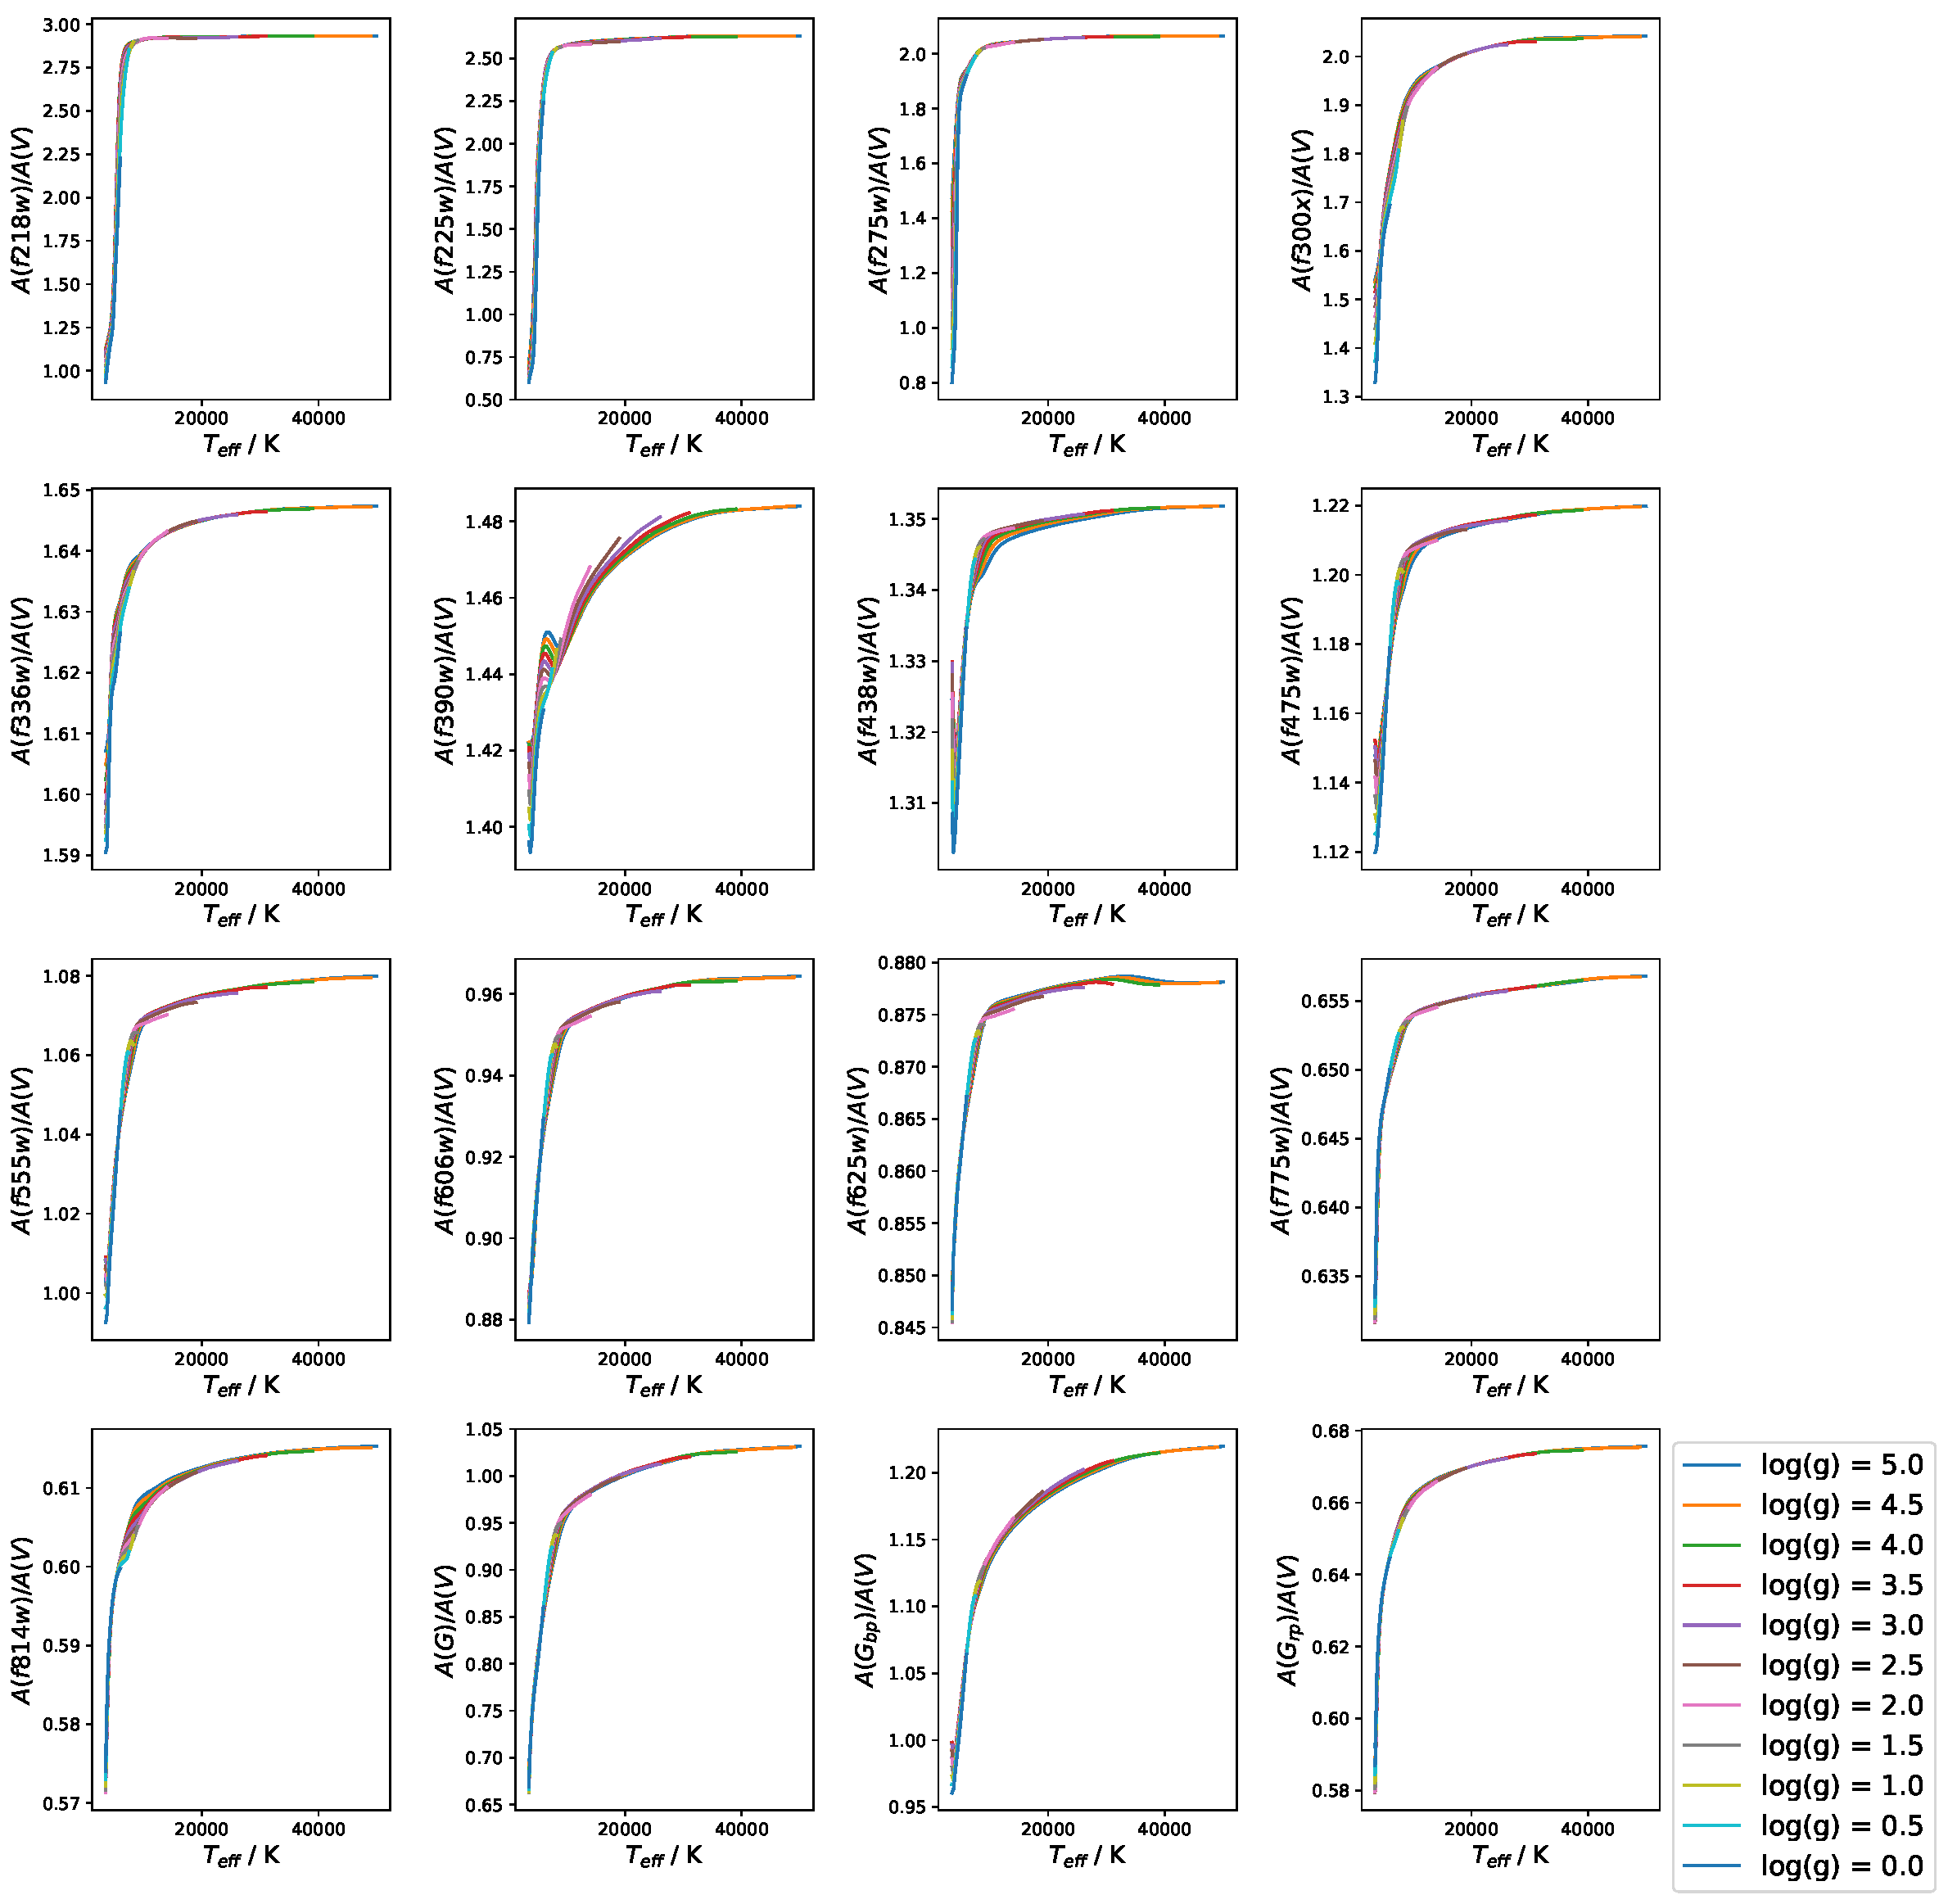
\includegraphics[width=1.0\textwidth]{../just_full_data/comb/AHub_FeH0p0_just_Teff_plot_lines.pdf}
\caption{Solar-metallicity extinction ratio data for the WFC3 (first 13 panels) and Gaia (last 3) systems, with point-to-point lines connecting datapoints for a fixed log($g$) value.}
\label{just_data_FeH0_WFC3gaia}
\end{center}
\end{figure}

\begin{figure}[h]
\begin{center}
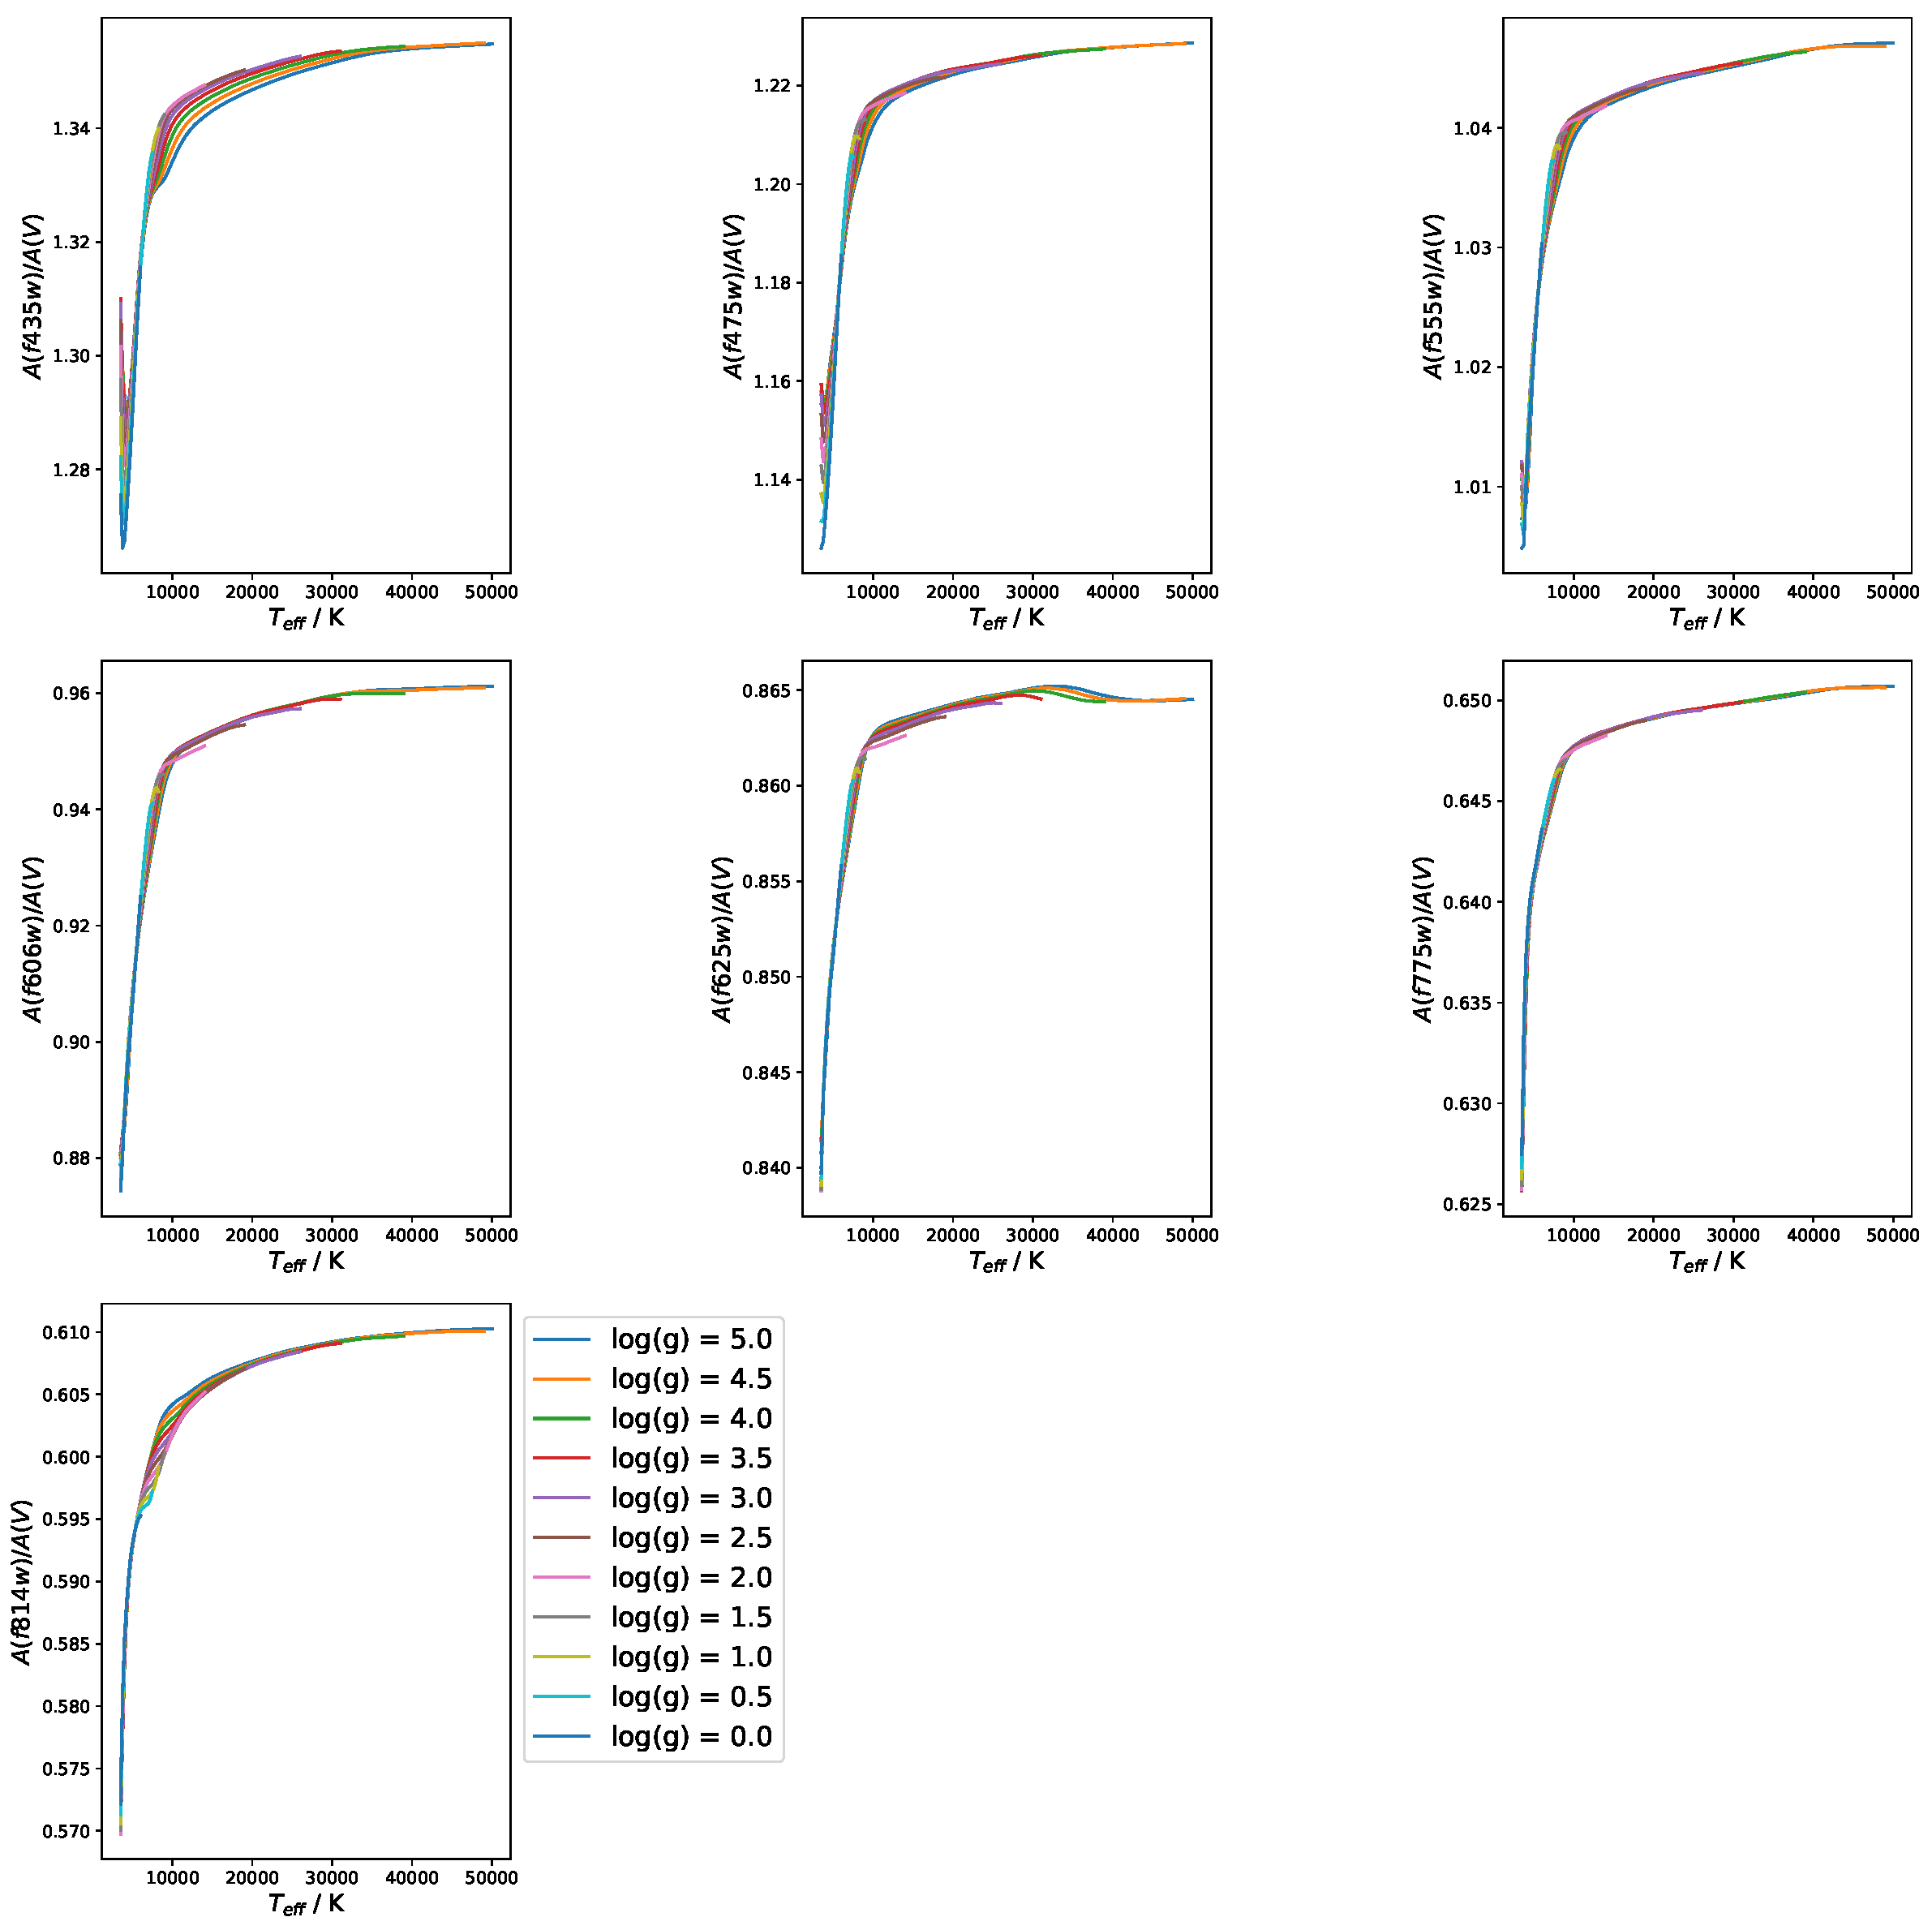
\includegraphics[width=1.0\textwidth]{../just_full_data/ACS/AHub_FeH0p0_just_Teff_plot_lines.pdf}
\caption{Same as Figure \ref{just_data_FeH0_WFC3gaia}, except the filters shown here are for the ACS system.}
\label{just_data_FeH0_ACS}
\end{center}
\end{figure}

A property found in the data for some filters, more pronounced at higher metallicity but with a possible slight dependence on surface gravity, is the tendency of the gradient of $A_{X}/A_{V}$ with increasing $T_{\textnormal{eff}}$ to become significantly less positive at the lowest temperatures in the data, typically around 4000K and below. The spread in $A_{X}/A_{V}$ values for different log($g$) is typically about 0.2-0.4, with a linear progression from log($g$) = 5.0 at the lowest end to log($g$) = 0.0 at the highest. In some filters, at the highest metallicity employed ([Fe/H] = 0.5), this phenomenon causes the gradient to invert and become significantly negative, reversing the trend everywhere else in the data, including for the same filters at lower metallicity. Due to the shape of the resulting point-to-point line in these axes, it has been dubbed the ``tail-flick'' phenomenon.\\*

This gradient inversion was ignored as an artefact from the numerical integration required for Equation \ref{BC_extinc}. This was justified on the basis that it is physical infeasible for a cooler star to experience a higher extinction $A_{X}$ than a hotter star for a globally-constant $A_{V}$ value and metallicity, as was assumed for data in each BC table. In the relevant filters, only effective temperatures above those affected by the gradient inversion was used for fitting.\\*

\section{Extinction ratio models} \label{ext_models}

In order to find usable model functions without running into issues with degeneracy between coefficients in the same function, prioritising the order in which the three stellar parameters were model was paramount. Too many coefficients created errors that were significantly greater in degenerate coefficients than in non-degenerate ones. This would obscure any useful information about the validity of the function form.\\*

The bolometric flux of a black body can be calculated as the total area under the curve described by the Planck function per unit wavelength/frequency as a function of wavelength/frequency  (see Equations \ref{planck_bb} and \ref{planck_bb_freq}). Since stellar emission spectra can be reasonably approximated by a black body emission with absorption lines, it can be seen from Equation\ref{Teff_def} that the greatest effect on stellar spectra, and therefore on the extinction coefficient, will come from changes in effective temperature. Therefore, the initial functions to be fitted were simple functions of $T_{\textnormal{eff}}$ only:

\begin{equation}
A_{\textnormal{pow}} (T_{\textnormal{eff}}) = a (T_{4})^{b} + c
\label{Teff_pow}
\end{equation}

\begin{equation}
A_{\textnormal{exp}} (T_{\textnormal{eff}}) = a \exp(b T_{4}) + c
\label{Teff_exp}
\end{equation}

where $T_{4} = 10^{-4} \times T_{\textnormal{eff}}$. The fitting operation was carried out on the data for solar metallicity ([Fe/H] = 0.0) and, because it gave the greatest number of $T_{\textnormal{eff}}$ data points, log($g$) = 5.0. This dataset will be referred to as the basic fitting data (BFD).\\*

****The results of this fitting process are detailed, for the cases where the fit was sufficiently accurate, in Table \ref{simpfunc_coeffs_table}. The table shows the filters and lists which of the two function forms provided the best fit for the relevant data, followed by the respective coefficient values and uncertainties. The final column lists the lowest $T_{\textnormal{eff}}$ value for which the given coefficient values is valid at all combinations of surface gravity and metallicity. \\*

For the data in the Gaia filters, the opportunity was taken to compare the models produced in this project with the models for $R_{X}$ for these same filters detailed by \cite{2018MNRAS.479L.102C}. To apply the \cite{2018MNRAS.479L.102C} model to the extinction ratios used for this project, the definition of $R_{X}$ was used to construct the following equation:

\begin{equation}
\frac{A_{X}}{A_{V}} = \frac{R_{X}}{R_{V}} = \frac{R_{X}}{3.1}
\label{convert_Rx_to_Ax}
\end{equation}

****Within the metallicity and temperature ranges for which the \cite{2018MNRAS.479L.102C} model is applicable, these models are in agreement with the ATLAS9 $A_{X}/A_{V}$ and with the models created for this project.\\*

There were filters whose BFD could not support an accurate fit or maintain the desired accuracy across all combinations of log($g$) and [Fe/H] using $A_{\textnormal{pow}}$ or $A_{\textnormal{exp}}$. For these filters, more intricate functions were sought, including functions with explicit dependences on $g$ and [Fe/H]. Several unsuccessful approaches were made before an acceptable function was found for each filter.\\*

The most successful approach was plotting all the available data for each filter, in multiple 2D and 3D axes, and analysing it visually. The trends seen in the data were transcribed to find not only an overarching function template, akin to the status of $A_{\textnormal{pow}}$ and $A_{\textnormal{exp}}$, but also smaller mathematical constructs within the template, such as describing a decay coefficient in terms of log($g$) and [Fe/H].\\*

The details of the final form of the template as a function of each stellar parameter were deduced by fitting a logistic function of $T_{\textnormal{eff}}$ to the $A_{X}/A_{V}$ data for each ([Fe/H],log($g$)) combination. This was decided on the basis that $A_{\textnormal{exp}}$ had been superior to $A_{\textnormal{pow}}$ in describing the data for these filters and because the low-$T_{\textnormal{eff}}$ change in gradient appeared to be more significant than for other filters. Furthermore, the gradient was not inverted, as can be seen in Figure \ref{just_data_FeH0_WFC3gaia}. Of particular importance was the fact that the $T_{\textnormal{eff}}$ gradient prior to the plateau appears to lead to an asymptote at lower, but still physically-viable, stellar effective temperatures. This issue is resolved by the logistic function's property of converging to a constant value for both very high and low values of the input variable. \\*

For a general logistic function in $T_{\textnormal{eff}}$, there are four key parameters:
\begin{itemize}
\item The global maximum value, denoted in this case by $A_{max}$;
\item The global minimum value, $A_{min}$;
\item The exponential decay coefficient, $k$;
\item The $T_{\textnormal{eff}}$-coordinate of the sigmoid midpoint, in this case $T_{\textnormal{0}}$.
\end{itemize}

It was confirmed that this new function could describe each scenario accurately enough for further analysis, ****as shown in Table \ref{UV_coeffs_table}. The resulting coefficients were tabulated and analysed for trends and, if found, the nature of those trends. This allowed for the incremental construction of sub-functions of log($g$) and [Fe/H], making the overall function, $A_{logis}$, sensitive to all three input stellar atmosphere parameters, with effective temperature having the greatest effect and the relative effects of the other parameters dependent on the best-fit values of the relevant coefficients.\\*

The sub-functions of log($g$) and [Fe/H], upon inspection of the coefficients for the $T_{\textnormal{eff}}$-only logistic function, were found to be simple functions of log($g$) and [Fe/H], independent of $T_{\textnormal{eff}}$ variations. This allowed for them to be used as the definitions of $T_{0}$ and $k$, as shown in Equations \ref{T0_eq} and \ref{decay_const_eq}, respectively.

\begin{align}
T_{\textnormal{0}} &= a\log(g) + b\left(\frac{\left[\textnormal{Fe/H}\right]}{\left|\left[\textnormal{Fe/H}\right]\right|^{1/2}}\right) + c \label{T0_eq}\\
k &= d\log(g) + e\left[\textnormal{Fe/H}\right] + f \label{decay_const_eq}\\
A_{logis}(T_{\textnormal{eff}},g,\left[\textnormal{Fe/H}\right]) &= \frac{(A_{max}-A_{min})}{( 1 + \exp{(-10^{-4} k(T_{\textnormal{eff}}-T_{\textnormal{0}})) ) )}} + A_{min} \label{A_logis_UV}
\end{align}

The final form was then subjected to a final fit on the entire $A_{X}/A_{V}$ dataset, covering the entire ($T_{\textnormal{eff}}$,  log($g$), [Fe/H]) parameter space available. $A_{logis}$ was able to accurately reproduce the behaviour of almost the entire dataset. The coefficients for Equations \ref{T0_eq}-\ref{A_logis_UV} are given in Table \ref{UV_coeffs_table}. \\*


\begin{table}
\begin{center}
\resizebox{\textwidth}{!}{\begin{tabular}{ccccccc}
\hline
System & Filter &  Function & & Coefficients & & $T_{\textnormal{min}}$ / K \\
 & & ($A_{\textnormal{pow}}$ or $A_{\textnormal{exp}}$) & $a$ & $b$ & $c$ & (global maximum error margin) \\
\hline
& F435W & exp & -0.144$\pm$0.031 & -2.159$\pm$0.360 & 1.352$\pm$0.002 & 3500(0.03) \\
& F475W & exp & -0.214$\pm$0.047 & -2.660$\pm$0.380 & 1.226$\pm$0.002 & 4000(0.025) \\
& F555W & exp & -0.0914$\pm$0.048 & -2.677$\pm$0.901 & 1.045$\pm$0.002 & 3500(0.01) \\
ACS & F606W & exp & -0.218$\pm$0.055 & -2.867$\pm$0.445 & 0.959$\pm$0.002 & 3500(0.01) \\
& F625W & exp & -0.072$\pm$0.078 & -3.332$\pm$2.000 & 0.865$\pm$0.002 & 3500(0.01) \\
& F775W & pow & -0.0035$\pm$0.0042 & -1.4878$\pm$1.5414 & 0.6507$\pm$0.0031 & 3500(0.01) \\
& F814W & pow & -0.007$\pm$0.005 & -1.374$\pm$0.830 & 0.611$\pm$0.003 & 3750(0.015) \\ \hline

& F336W & pow & -0.0074$\pm$0.0041 & -1.5251$\pm$0.7272 & 1.6478$\pm$0.003 & 3500(0.025) \\
& F390W & exp & -0.0695$\pm$0.0057 & -0.6438$\pm$0.177 & 1.489$\pm$0.005 & 4500(0.04) \\
& F438W & exp & -0.1132$\pm$0.0658 & -3.0839$\pm$1.0322 & 1.3504$\pm$0.0017 & 3750(0.015) \\
& F475W & pow & -0.0179$\pm$0.0037 & -1.718$\pm$0.275 & 1.220$\pm$0.003 & 4000(0.02) \\
WFC3 & F555W & pow & -0.0138$\pm$0.0033 & -1.8873$\pm$0.3326 & 1.0798$\pm$0.0024 & 3750(0.02) \\
& F606W & exp & -0.2131$\pm$0.0559 & -2.8788$\pm$0.4604 & 0.9623$\pm$0.0017 & 3500(0.015) \\
& F625W & pow & -0.0042$\pm$0.0031 & -2.0634$\pm$1.0248 & 0.8787$\pm$0.0022 & 3500(0.01) \\
& F775W & pow & -0.0033$\pm$0.0041 & -1.529$\pm$1.6335 & 0.6568$\pm$0.003 & 3750(0.01) \\
& F814W & pow & -0.0071$\pm$0.0046 & -1.3905$\pm$0.8027 & 0.6158$\pm$0.0034 & 4000(0.01) \\ \hline

& G & pow & -0.0888$\pm$0.0045 & -1.402$\pm$0.0642 & 1.0395$\pm$0.0033 & ****0(0.0) \\
Gaia & G\textsubscript{bp} & pow & -0.115$\pm$0.0081 & -0.8997$\pm$0.0692 & 1.2468$\pm$0.0068 & ****0(0.0) \\
& G\textsubscript{rp} & pow & -0.0159$\pm$0.0047 & -1.3519$\pm$0.3678 & 0.6772$\pm$0.0035 & ****0(0.0) \\ \hline

\end{tabular}}
\caption{Coefficient values produced for each filter via $A_{\textnormal{exp}}$ or $A_{\textnormal{exp}}$ fitting, as appropriately labelled. Any filters missing from this table are those with data that could not be accurately fitted using either function. The errors are calculated using a simulated $A_{X}/A_{V}$ uncertainty of 0.01. ****The final column displays the lowest effective temperature for which the given model and coefficients were able to describe the $A_{X}/A_{V}$ data across all values of log($g$) and [Fe/H]}
\label{simpfunc_coeffs_table}
\end{center}
\end{table}

The extinction-ratio data for all filters, with the exception of the four fully-UV filters in the WFC3 system, could be accurately modelled by the simplest functions trialled for fitting, $A_{\textnormal{exp}} (T_{\textnormal{eff}})$ or $A_{\textnormal{pow}} (T_{\textnormal{eff}})$.

\begin{table}
\begin{center}
\begin{tabular}{ccccc}
\hline
\multirow{2}{*}{Coefficient} & \multicolumn{4}{c}{Filter} \\
 & F218W & F225W & F275W & F300X \\
\hline
$a$ & -120.9$\pm$4.1 & -97.21$\pm$3.85 & -239.0$\pm$12.0 & -302.1$\pm$45.0 \\
$b$ & 467.6$\pm$7.9 & 357.2$\pm$7.9 & 236.0$\pm$20.4 & 350$\pm$125 \\
$c$ & 5673$\pm$16 & 4967$\pm$22 & 4161$\pm$79 & 4270$\pm$913 \\
$d$ & 1.435$\pm$0.209 & -0.174$\pm$0.136 & -2.117$\pm$0.326 & -0.176$\pm$0.087 \\
$e$ & -3.211$\pm$0.382 & -2.691$\pm$0.256  & -2.140$\pm$0.445 & -0.352$\pm$0.115 \\
$f$ & 19.19$\pm$0.62 & 18.62$\pm$0.55  & 22.20$\pm$1.48 & 4.315$\pm$0.529 \\
$A_{min}$ & 1.026$\pm$0.012 & 0.337$\pm$0.028 & 0.409$\pm$0.113 & 1.000$\pm$0.199 \\
$A_{max}$ & 2.909$\pm$0.003 & 2.581$\pm$0.003 & 2.030$\pm$0.003 & 2.015$\pm$0.004 \\
\hline
Max. deviation in $A_{X}/A_{V}$ & 0.25 & 0.3 & 0.2 & 0.15 \\
%($T_{\textnormal{eff}}$ / K, & & & None & None \\
%log($g$) / dex, & & & None & None \\
%$\textnormal{[Fe/H]}$) & & & None & None \\
%exceptions & & & & \\
\hline
\end{tabular}
\caption{Coefficient values for non-trivial $A_{X}/A_{V}$ functions, as described in Equations \ref{T0_eq}-\ref{A_logis_UV}, produced for fitting to UV filter data. The bottom row represents the global maximum deviation from the data.}
\label{UV_coeffs_table}
\end{center}
\end{table}

All the functions are consistent with the general trends predicted by the physics in stellar atmospheres, since the effective temperature has the greatest effect upon the value of $A_{X}/A_{V}$, with relatively minor effects due to spectral absorption lines, via surface gravity and metallicity. In general stars with higher effective temperatures (and consequently stronger and bluer flux spectra) experience higher $A_{X}/A_{V}$ values in all filters than stars with low effective temperatures. The maximum $A_{X}/A_{V}$ value in a given filter decreases as the filter's central wavelength increases. This is expected for black-body analogues (see Equation \ref{planck_bb} and Figure \ref{planck_curve}). Both trends are also consistent with the known short-wavelength preference of physical mechanisms causing interstellar extinction.\\*

The accuracy of these relatively simple functions is important because the $A_{X}/A_{V}$ dataset for each filter is now reduced to a much smaller number of degrees of freedom, equal to the number of coefficients in the relevant function. The input parameters ($T_{\textnormal{eff}}$, log($g$) and [Fe/H]) are required regardless of whether interpolation of the tables of $A_{X}/A_{V}$ data or the functions are being employed, and so they make no difference in comparing the information complexity of the tables versus the functions.\\*


\section{Effect on isochrones} \label{result_CMDs}
The equations detailed in Section \ref{isoc_fit} were used to convert the model parameters listed in the BaSTI data to the stellar parameters used by the $A_{X}/A_{V}$ functions in this project. \\*

The ATLAS9 metallicity chosen for calculating the fixed-extinction $A_{X}/A_{V}$ values to be applied to the isochrone was the value which best matched the metallicity of the isochrone to which the coefficient was applied. The ATLAS9 value will be denoted [Fe/H]$_{CM}$. The first value was equal to $(A_{X}/A_{V})_{plat} = (A_{X}/A_{V})(T_{\textnormal{eff}} = 50,000\textnormal{K},\log(g) = 5.0,\textnormal{[Fe/H]}_{CM})$, and the second was equal to $(A_{X}/A_{V})_{MS} = (A_{X}/A_{V})(T_{\textnormal{eff}} = 5,000\textnormal{K},\log(g) = 5.0,\textnormal{[Fe/H]}_{CM})$. This was done to reflect the fact that, for the first case, the assumption of a constant extinction coefficient is valid in the plateau region and, for the second, the fact that, given the position of the MSTO in terms of stellar $T_{\textnormal{eff}}$ values, it would be more prudent to ensure that the upper main sequences resulting from both approaches to extinction coincide in the CMD, making it easier to see any disagreements in the turn-off ages. For each of these plots, $A_{V}$ was fixed at a value of 1.0.\\*

In each of the CMDs, the extinction ratio functions have been applied to a solar-metallicity ([Fe/H] = 0), 500 Myr isochrone, which is shown as a solid orange line. A fixed extinction ratio has been applied to three solar-metallicity isochrones with ages of 400 (solid green), 500 (solid blue) and 600 (solid red) Myr, respectively. A solar-metallicity, 500 Myr isochrone with zero extinction is added for illustration purposes as a solid purple line.\\*

\subsection{ACS} \label{ACS_isoc}
The CMD chosen for the ACS was the F435W-(F435W-F814W) axis combination. This CMD is useful as it pairs the bluest and reddest wide-field filters for the ACS in its colour index, which is the index most likely to distinguish between objects with a large range of effective temperatures, making it useful for modelling the main sequence and MSTO, the two most important CMD components for calculating cluster isochrone ages. This CMD corresponds, by design, to the pre-existing Johnson-Cousins $B$-($B-I$) CMD \citep{2005PASP..117.1049S}, which allows direct comparison of observed data with archive data obtained before the creation of the HST filters.

\begin{figure}[h]
\begin{center}
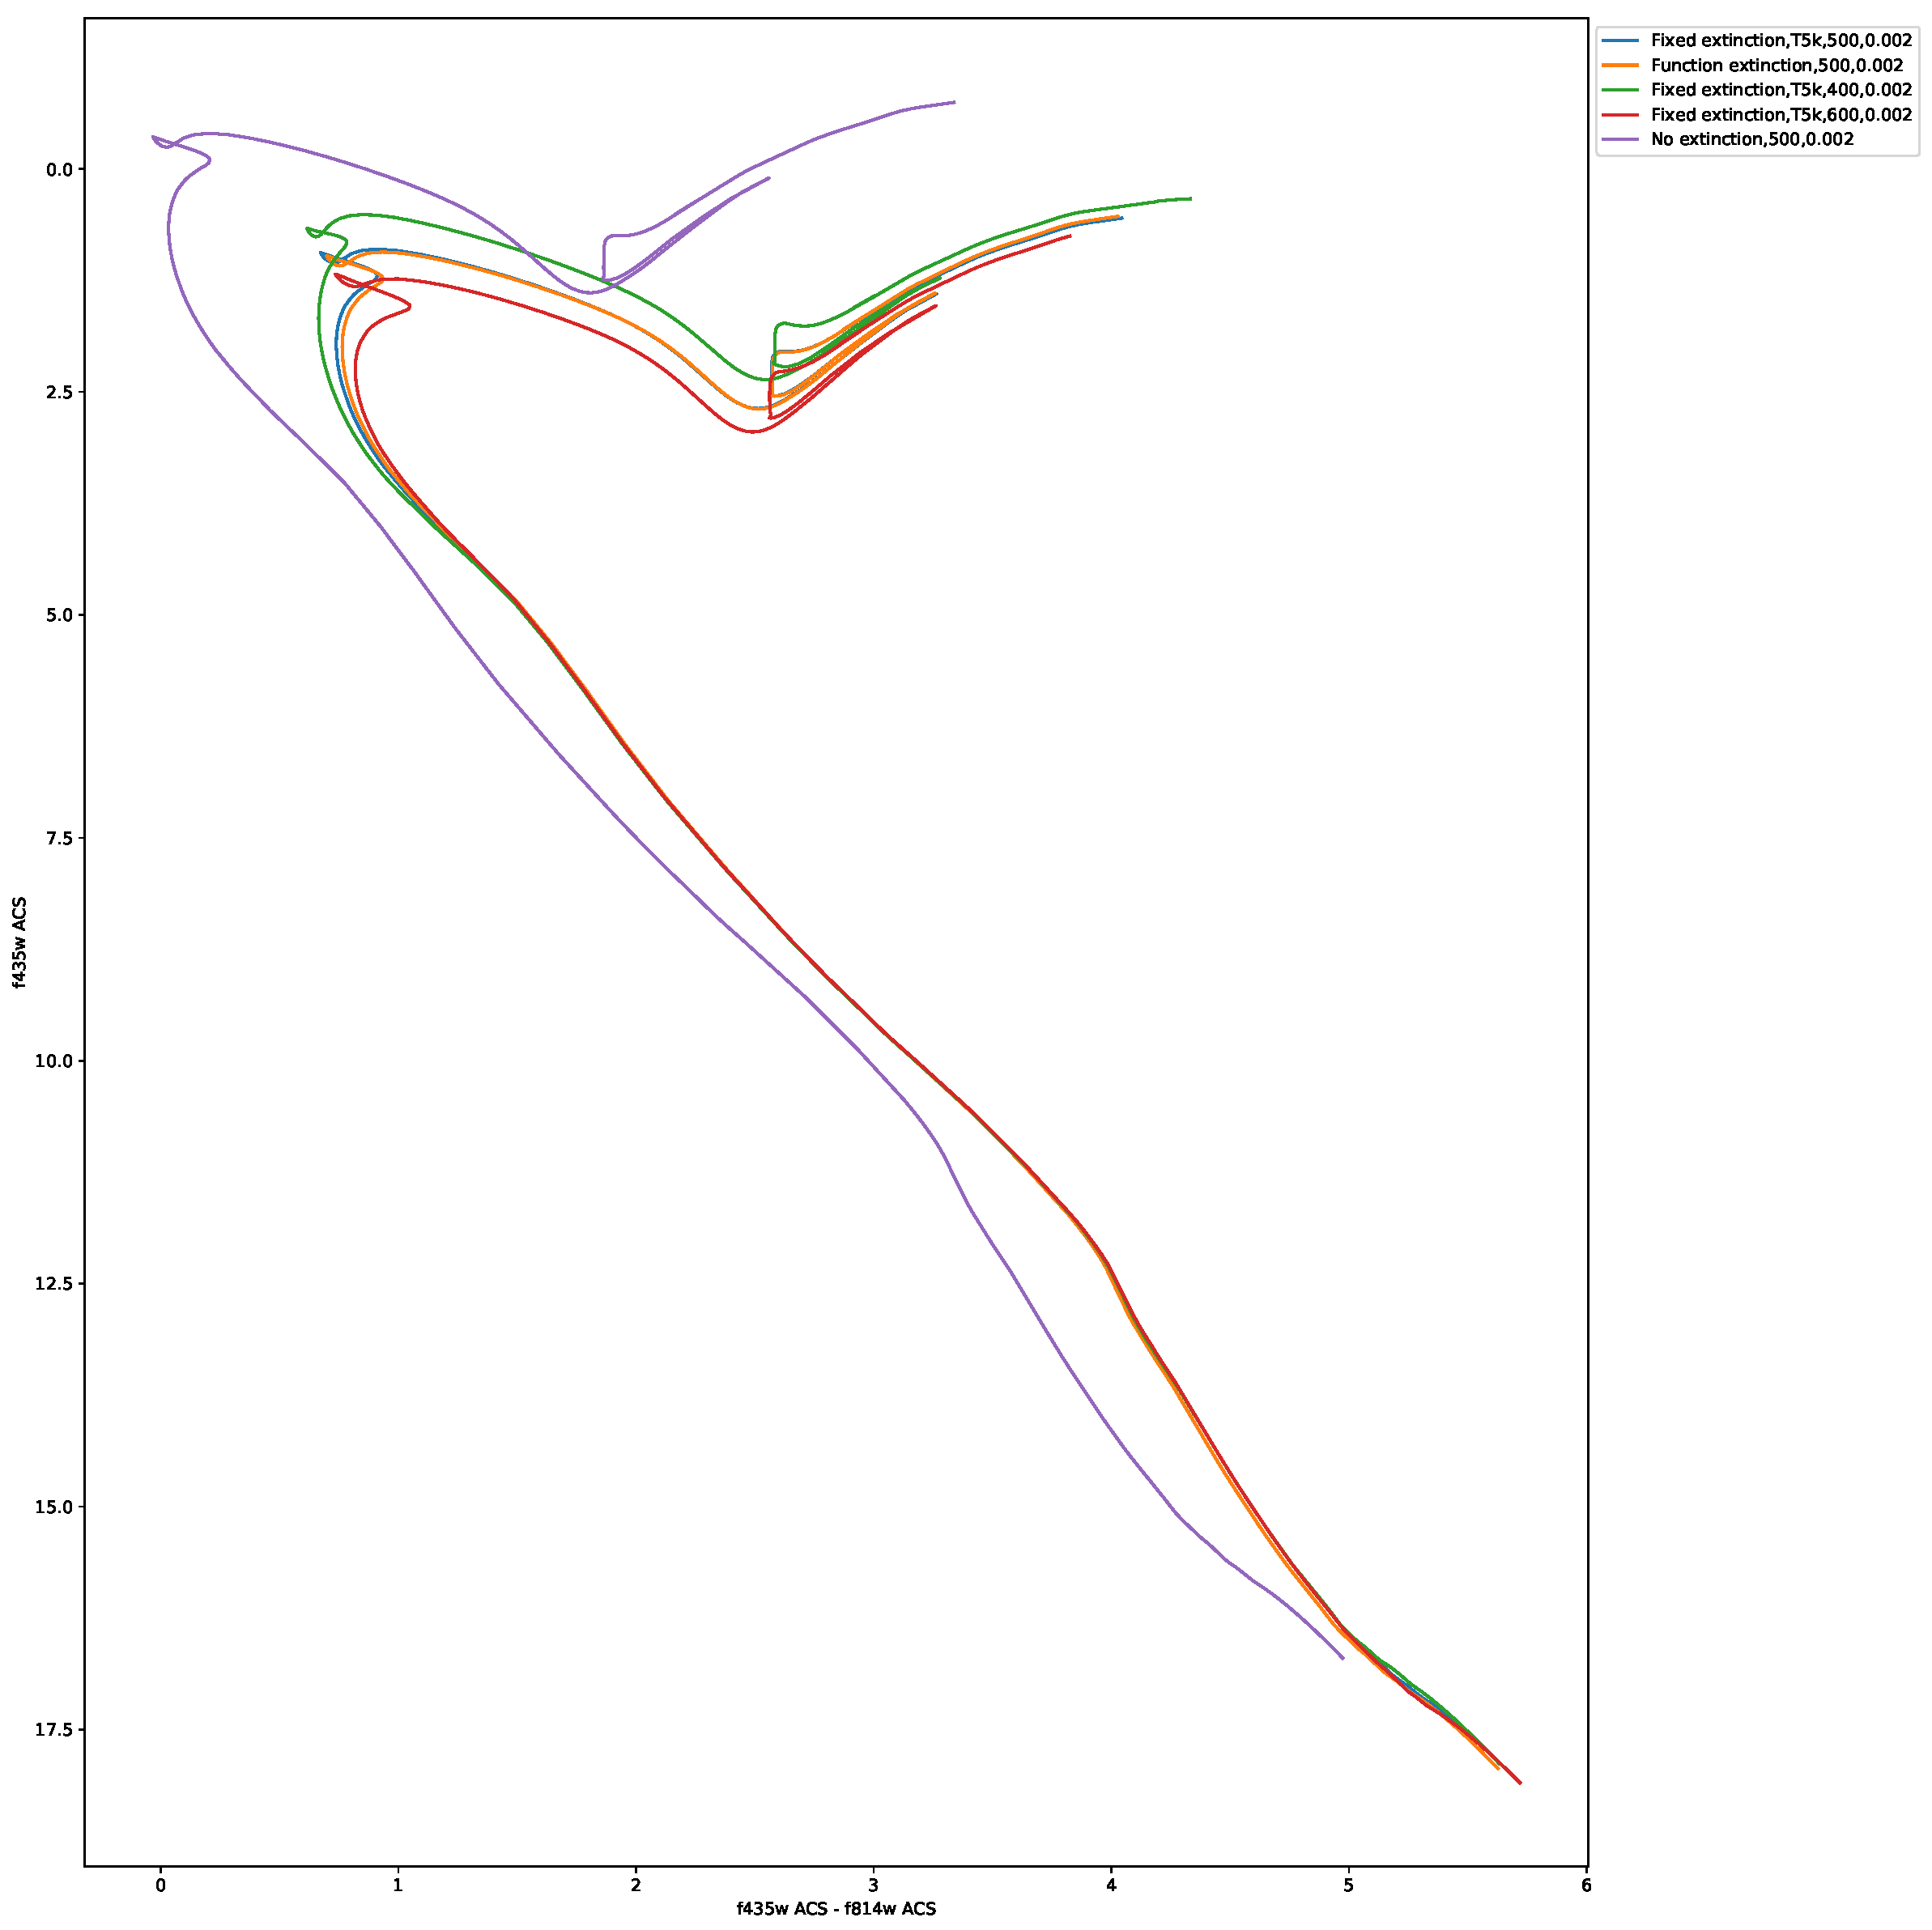
\includegraphics[width=1.0\textwidth]{../basti_isochrones_10_13Gyr/Extinction_T5k_FeH0fix_func_f435wACS_f435wACSmf814wACS_500_400_600_Myr_FeH_0p002_ref_noext_Av_1p0.pdf}
\caption{ACS F435W-(F435W-F814W) CMD with a fixed extinction ratio equal to $(A_{X}/A_{V})_{MS}$ for each filter}
\label{acs_isoc_T5k}
\end{center}
\end{figure}

\begin{figure}[h]
\begin{center}
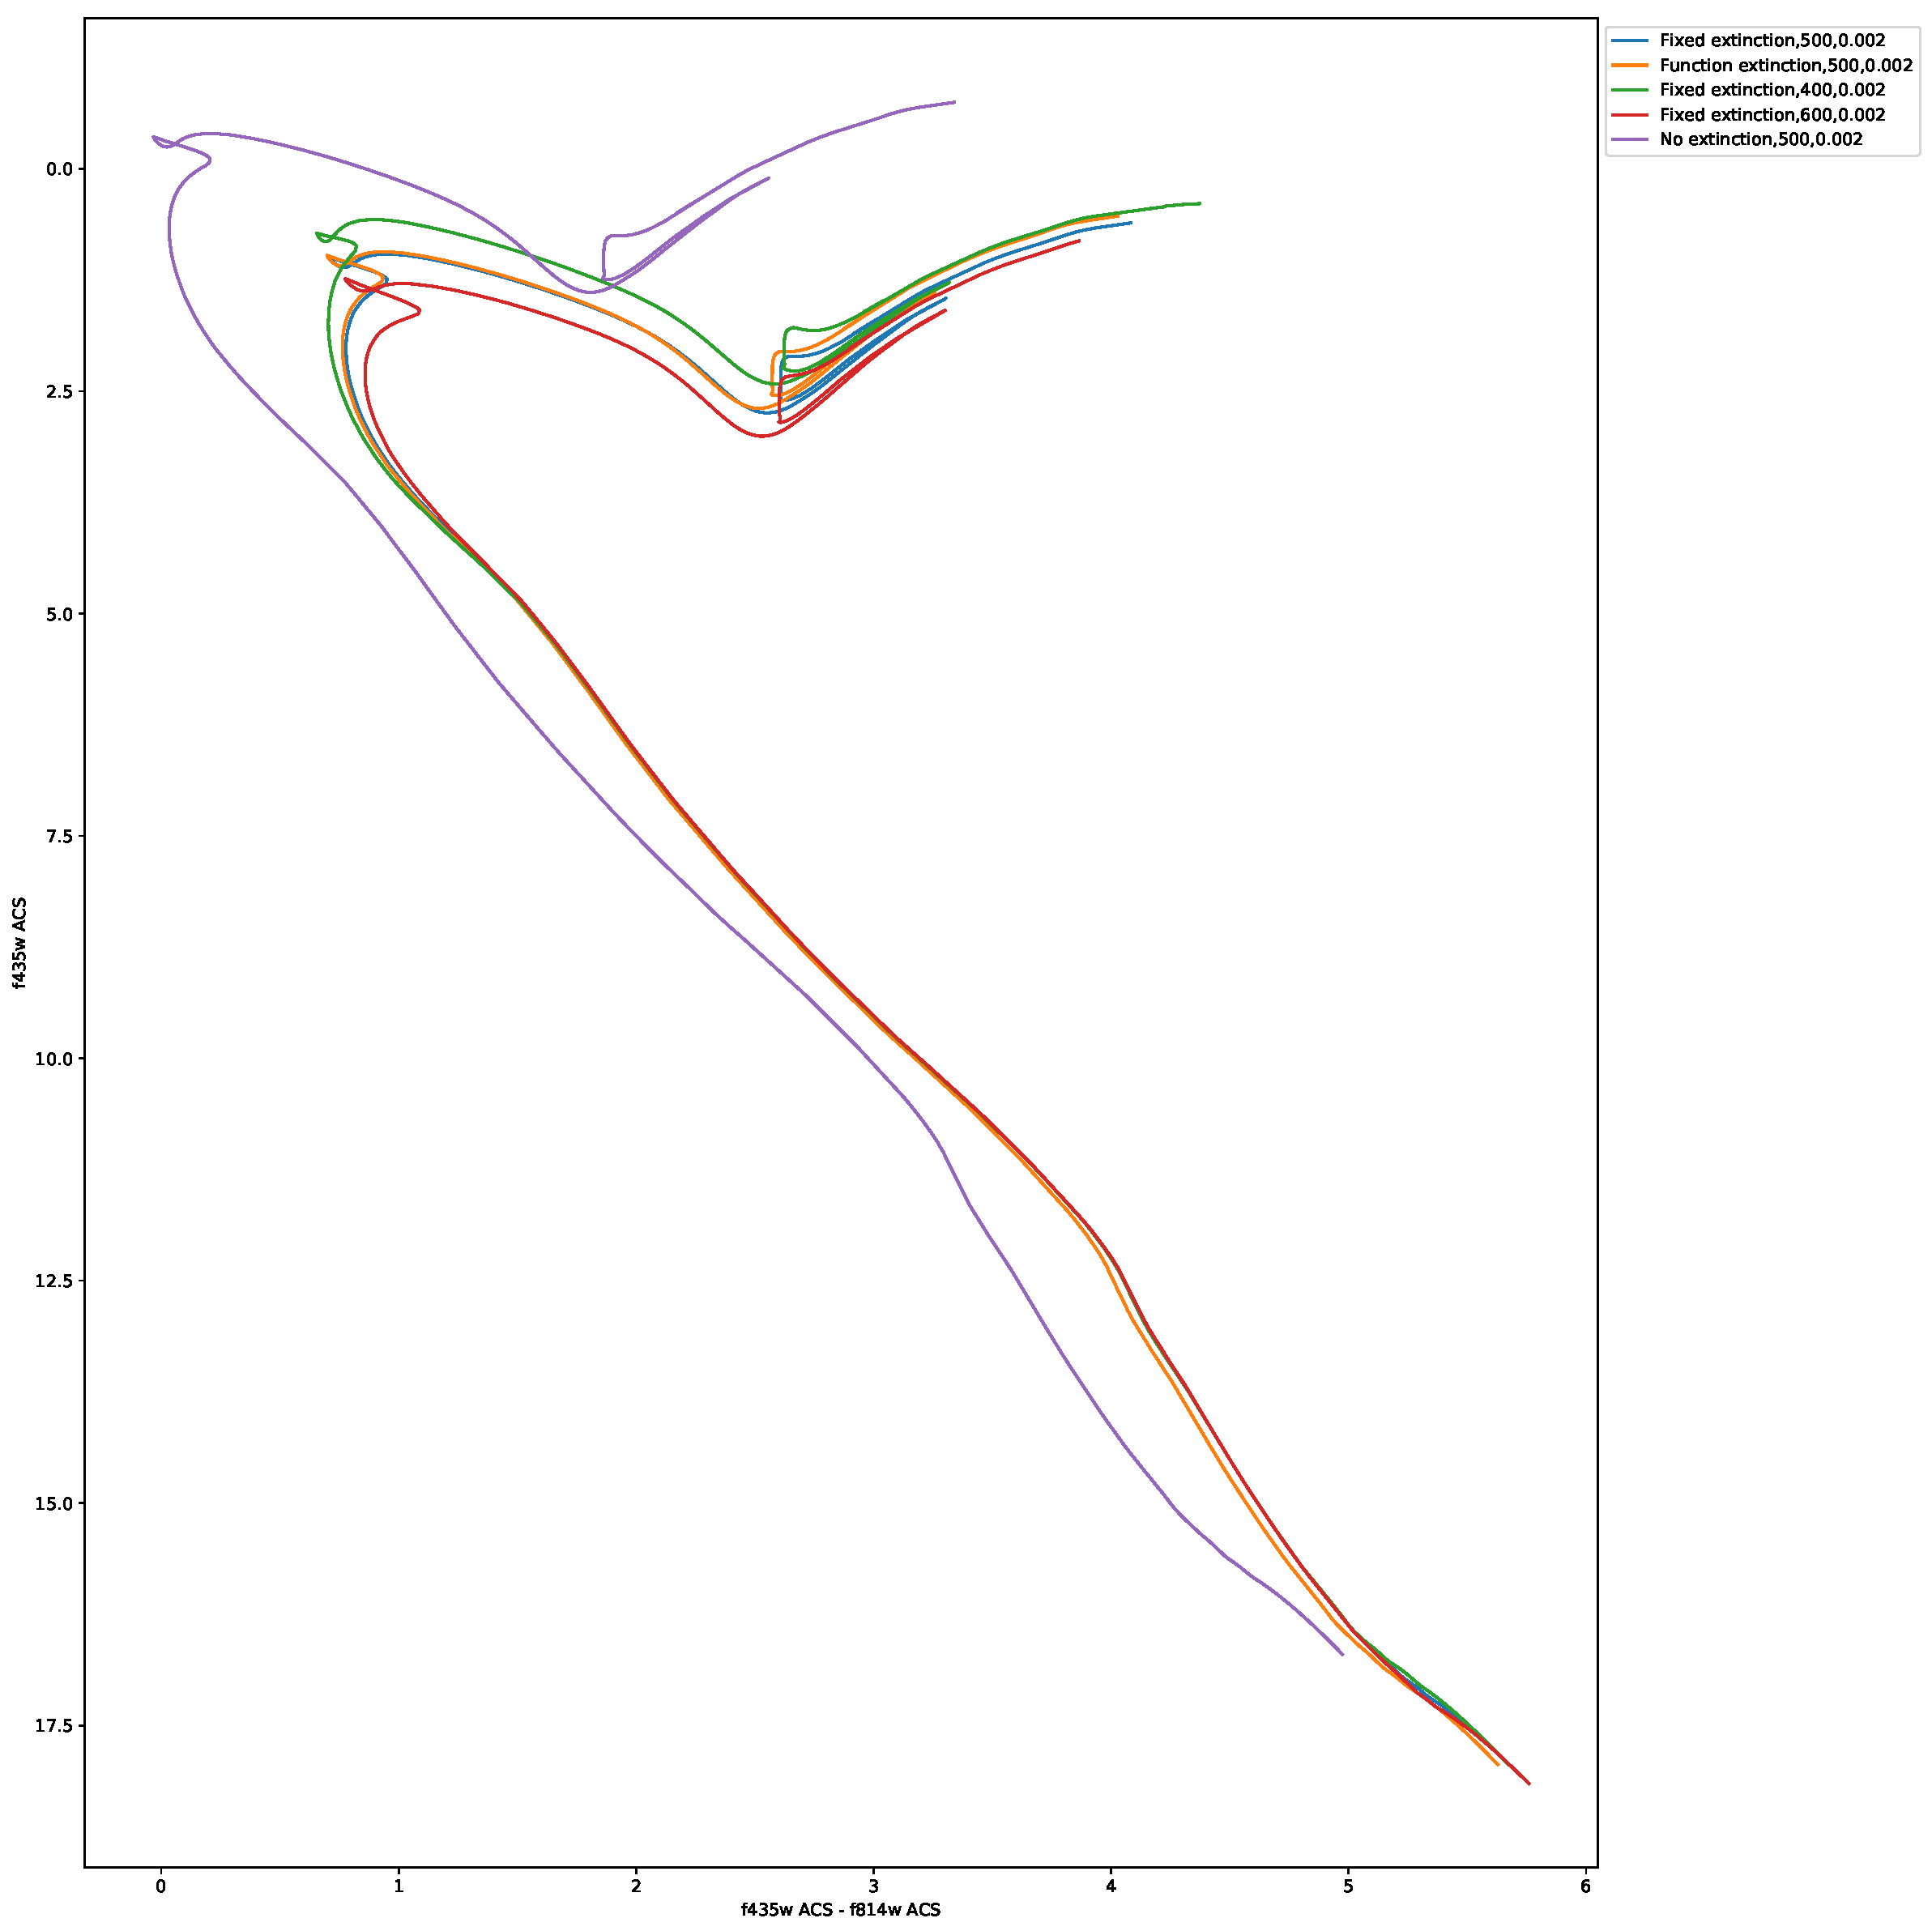
\includegraphics[width=1.0\textwidth]{../basti_isochrones_10_13Gyr/Extinction_T50k_FeH0fix_func_f435wACS_f435wACSmf814wACS_500_400_600_Myr_FeH_0p002_ref_noext_Av_1p0.pdf}
\caption{ACS F435W-(F435W-F814W) CMD with a fixed extinction ratio equal to $(A_{X}/A_{V})_{plat}$ for each filter}
\label{acs_isoc_T50k}
\end{center}
\end{figure}

It can be seen in Figure \ref{acs_isoc_T5k} that the impact of changing the extinction approach used to change the isochrone position in this CMD is insignificant. Although there are some larger differences in the position of the isochrone in the post-sub-giant branch (SGB) evolutionary stages, this is irrelevant when determining the isochrone age of an observed stellar population.\\*

The result of using $(A_{X}/A_{V})_{plat}$ is not significantly different from that of using $(A_{X}/A_{V})_{MS}$ for this CMD. It can be seen that any changes in $A_{X}/A_{V}$ values in the F435W and F814W ACS filters at different temperatures (see Figure \ref{just_data_FeH0_ACS}) are insignificant compared to the range of magnitudes covered by the isochrones in Figures \ref{acs_isoc_T5k} and \ref{acs_isoc_T50k}.\\*

\subsection{WFC3} \label{WFC3_isoc}

Two different CMDs were chosen whose filters are part of the WFC3. The first CMD is the F555W-(F555W-F814W) axis combination. This CMD pairs a wide yellow filter (F555W) with the WFC3's reddest IR wide-field filter. This CMD mimics the pre-existing and widely-used Johnson-Cousins $V$-($V-I$) CMD \citep{2014wfc..rept...16S}, which allows direct comparison of observed data with archive data obtained before the creation of the HST filters.\\*

As with the previous ACS CMD, this CMD shows no significant changes in isochrone position resulting from either employing a FBER model or changing the extinction ratio value used for the fixed-value extinction model from $(A_{X}/A_{V})_{plat}$ to $(A_{X}/A_{V})_{MS}$ or vice versa.\\*

\begin{figure}[h]
\begin{center}
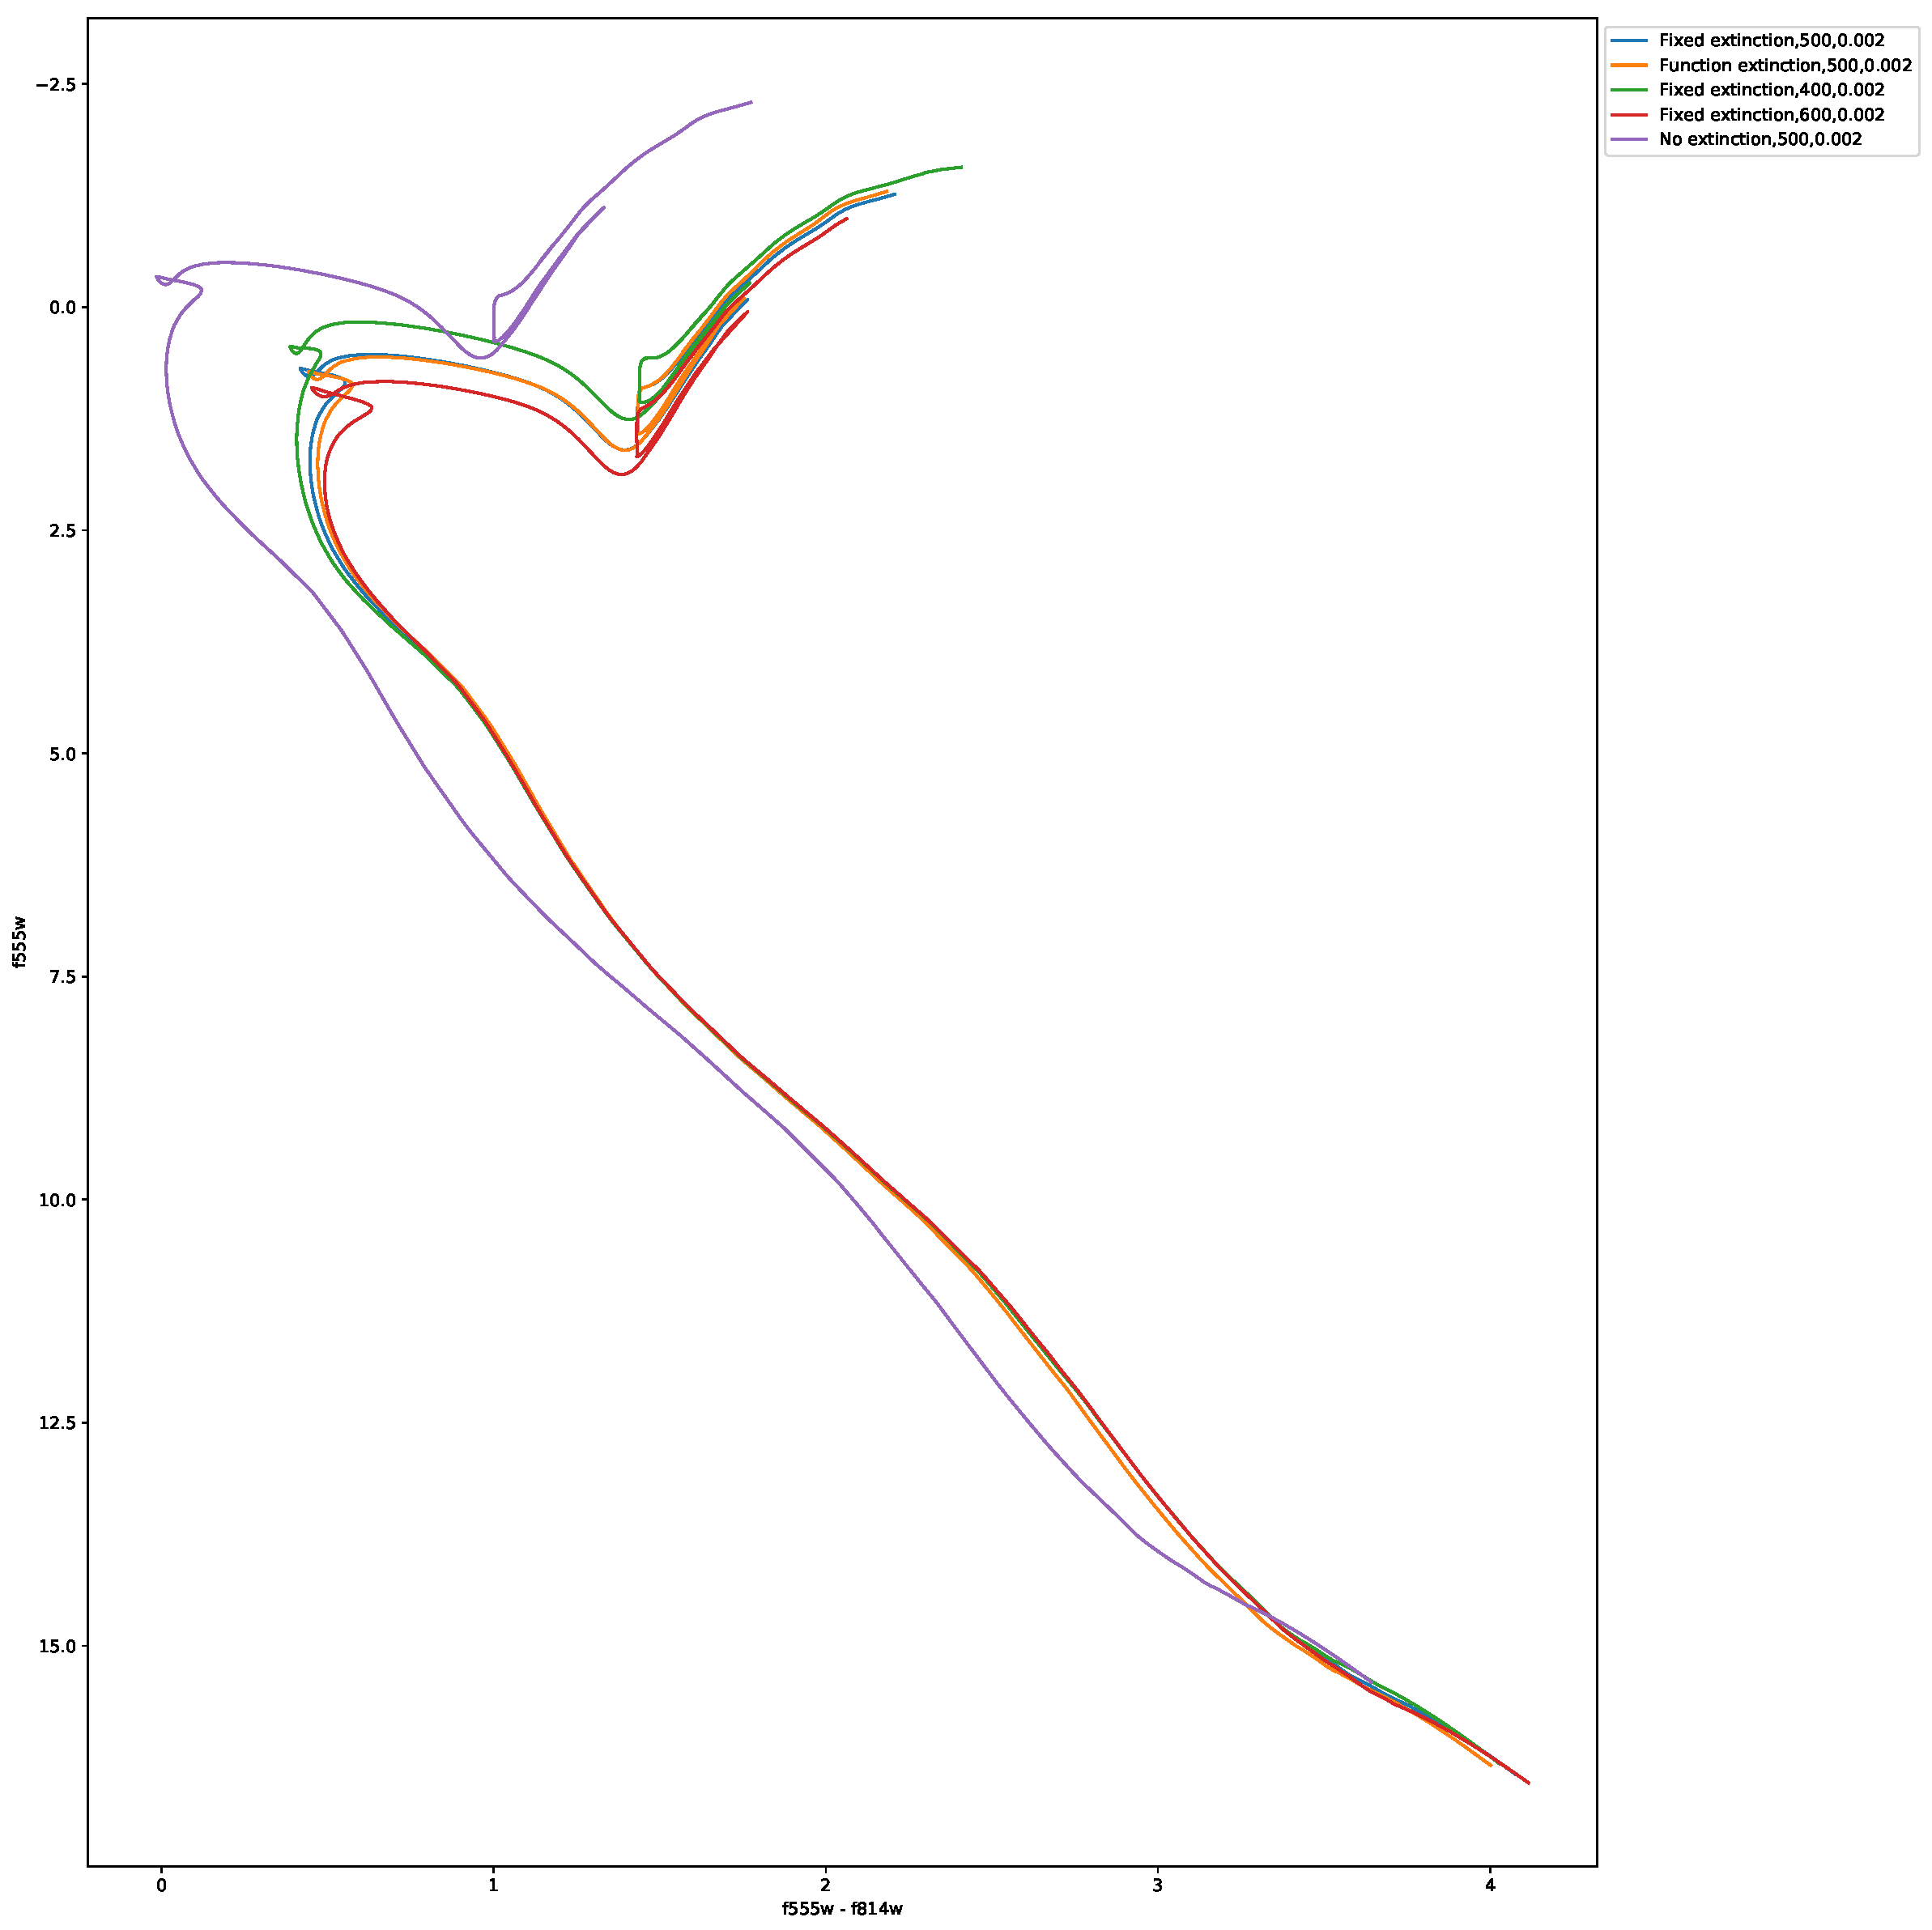
\includegraphics[width=1.0\textwidth]{../basti_isochrones_10_13Gyr/Extinction_T5k_FeH0fix_func_f555w_f555wmf814w_500_400_600_Myr_FeH_0p002_ref_noext_Av_1p0.pdf}
\caption{WFC3 F555W-(F555W-F814W) CMD with a fixed extinction coefficient equal to $(A_{X}/A_{V})_{MS}$ for each filter}
\label{wfc3_isoc1_T5k}
\end{center}
\end{figure}

\begin{figure}[h]
\begin{center}
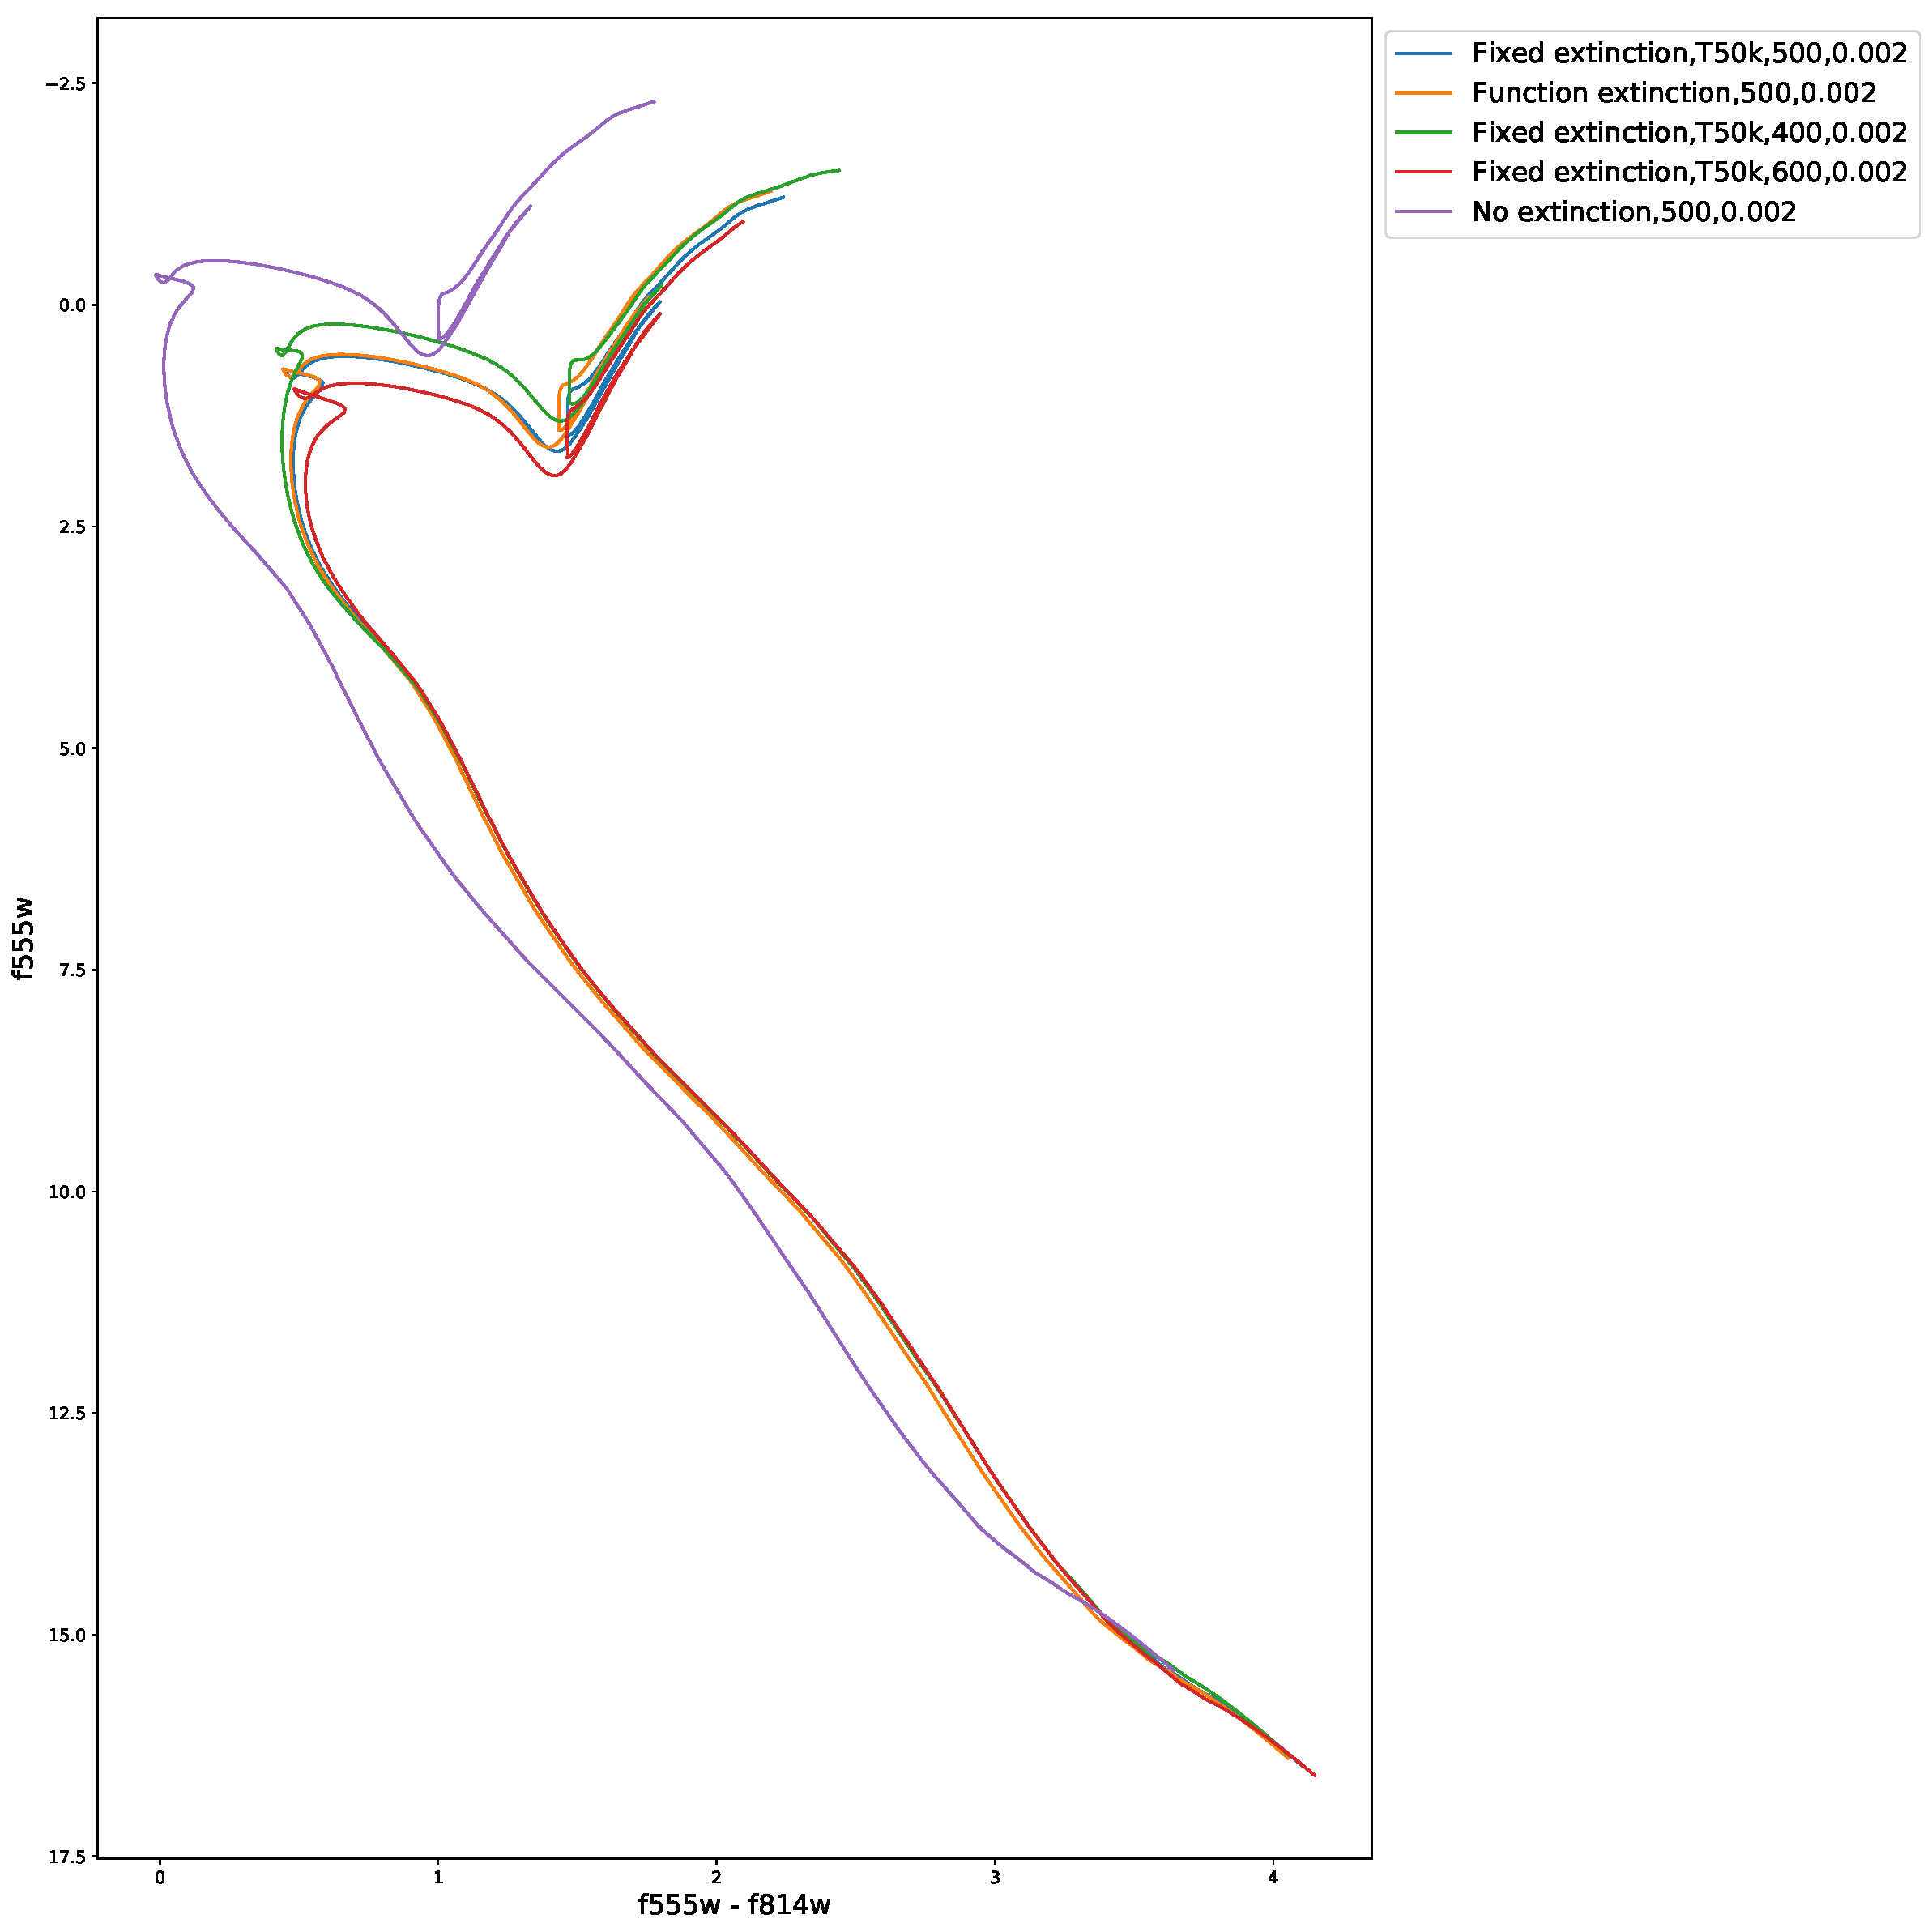
\includegraphics[width=1.0\textwidth]{../basti_isochrones_10_13Gyr/Extinction_T50k_FeH0fix_func_f555w_f555wmf814w_500_400_600_Myr_FeH_0p002_ref_noext_Av_1p0.pdf}
\caption{WFC3 F555W-(F555W-F814W) CMD with a fixed extinction coefficient equal to $(A_{X}/A_{V})_{plat}$ for each filter}
\label{wfc3_isoc1_T50k}
\end{center}
\end{figure}

The second WFC3 CMD that was studied is the F814W-(F275W-F814W) axis combination. The filters that form this CMD cover the soft-UV and near-IR regions of the EM spectrum. The high baseline wavelength coverage of this combination of filters makes the colour index sensitive to differences in $T_{\textnormal{eff}}$ in the hot horizontal branch (HB) stars. These objects are important due to direct helium abundance measurements (from absorption lines) being available in globular clusters only for HB stars with 8000 K $\lesssim T_{\textnormal{eff}} \lesssim$ 11500 K \citep{2018MNRAS.475.4088L}.

\begin{figure}[h]
\begin{center}
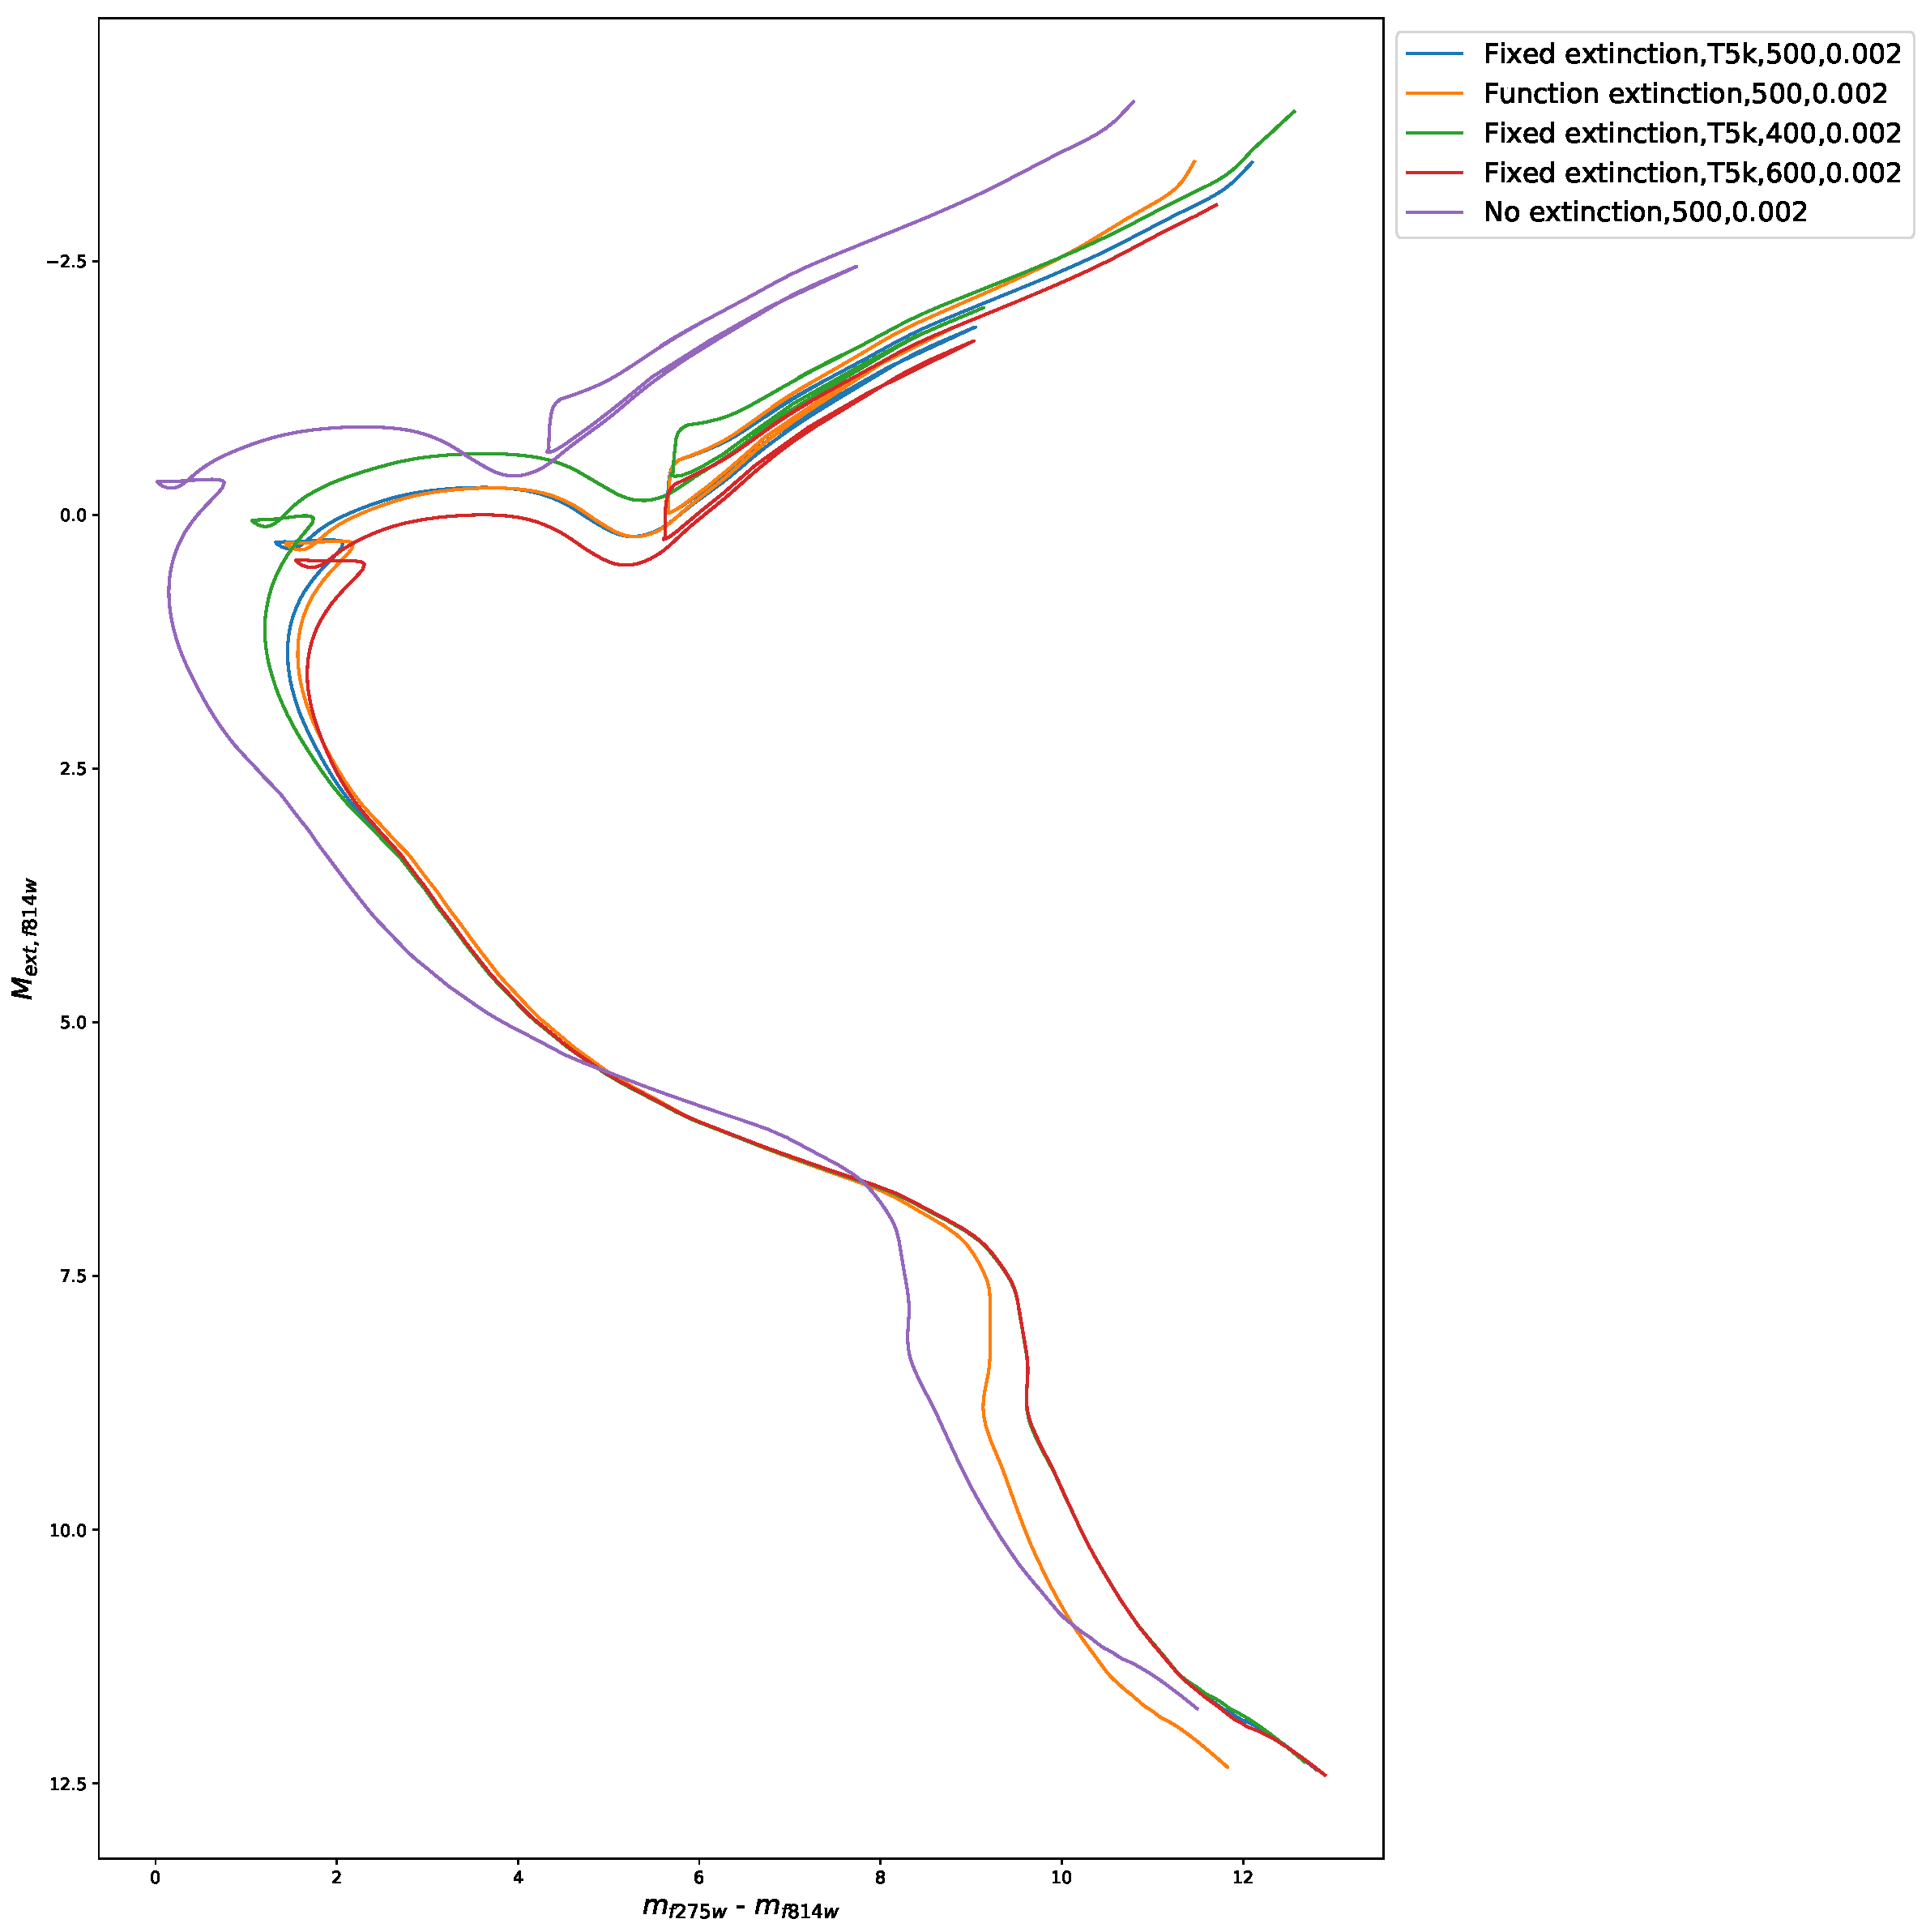
\includegraphics[width=1.0\textwidth]{../basti_isochrones_10_13Gyr/Extinction_T5k_FeH0fix_func_f814w_f275wmf814w_500_400_600_Myr_FeH_0p002_ref_noext_Av_1p0.pdf}
\caption{WFC3 F814W-(F275W-F814W) CMD with a fixed extinction coefficient equal to $(A_{X}/A_{V})_{MS}$ for each filter.}
\label{wfc3_isoc2_T5k}
\end{center}
\end{figure}

\begin{figure}[h]
\begin{center}
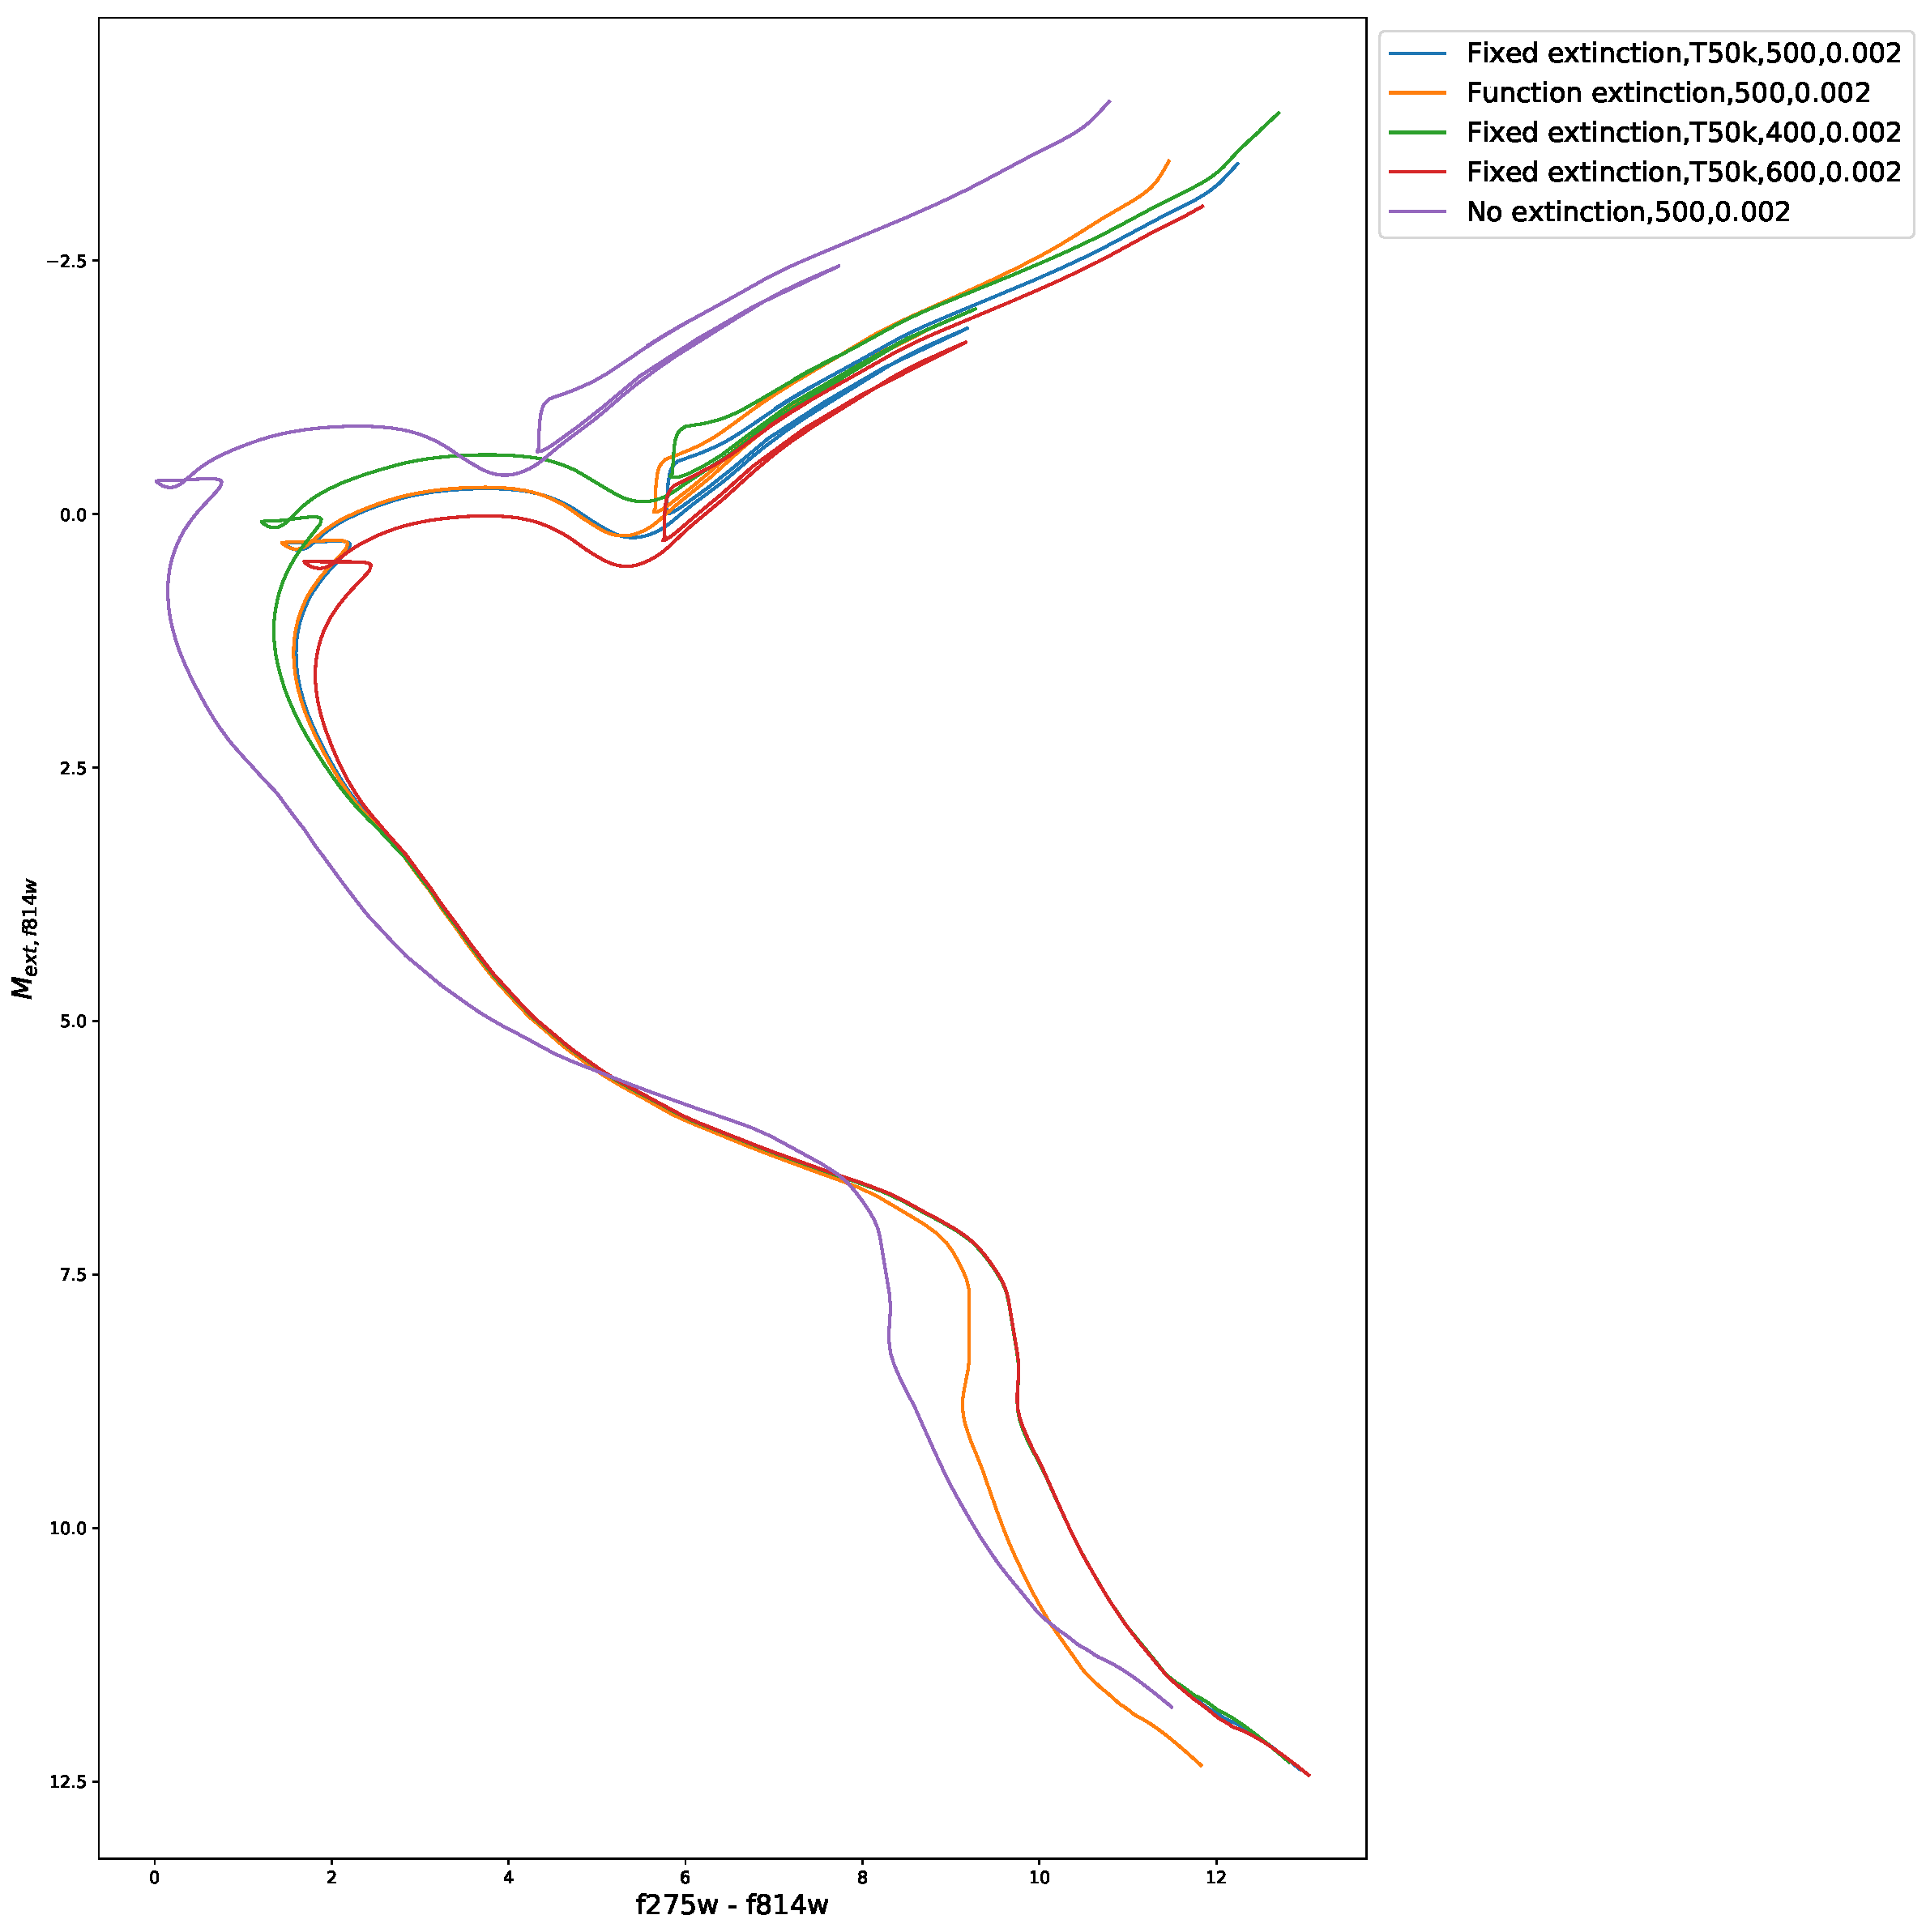
\includegraphics[width=1.0\textwidth]{../basti_isochrones_10_13Gyr/Extinction_T50k_FeH0fix_func_f814w_f275wmf814w_500_400_600_Myr_FeH_0p002_ref_noext_Av_1p0.pdf}
\caption{WFC3 F814W-(F275W-F814W) CMD with a fixed extinction coefficient equal to $(A_{X}/A_{V})_{plat}$ for each filter}
\label{wfc3_isoc2_T50k}
\end{center}
\end{figure}

In Figure \ref{wfc3_isoc2_T5k}, it can be seen that, when the models' upper main sequences are aligned (i.e., the $(A_{X}/A_{V})_{MS}$ fixed model is being used as a reference), the position of the MSTO of the FBER 500 Myr isochrone aligns with that of the 600 Myr fixed-ratio isochrone. By the point at which the SGB hook \citep{1998MNRAS.298..525P} appears, the FBER isochrone has almost realigned with the 500 Myr fixed-ratio isochrone. There are significant differences between the two 500 Myr isochrones after the lower portion of the RGB. In the lower main sequence, all isochrones with fixed extinction ratios appear significantly redder, while more or less maintaining their F814W magnitudes. This can only be the result of significant differences in $A_{F275W}/A_{V}$ values between models in the upper main sequence (higher $T_{\textnormal{eff}}$ values) and in the lower main sequence (lower $T_{\textnormal{eff}}$ values), as these differences are not reflected in the fixed-extinction models. \\*

In Figure \ref{wfc3_isoc2_T50k}, the temperature of 50,000 K used for $(A_{X}/A_{V})_{plat}$ increases the extinction ratio values in the fixed-extinction isochrones, shifting them down and to the right. Ironically, this higher $T_{\textnormal{eff}}$ value, which is far greater than any $T_{\textnormal{eff}}$ values present in the isochrone data, brings the MSTO positions of the two 500 Myr isochrones back into alignment. However, the use of $(A_{X}/A_{V})_{plat}$ increases the lower main sequence gap between the fixed-extinction isochrones and the FBER example. The disagreement between the 500 Myr isochrones now begins earlier in the evolutionary cycle, at the base of the RGB. \\*

Furthermore, there is a possibility of the lower main sequence disagreement between extinction treatment methods causing a disagreement in the estimated cluster metallicity, as the CMD position of this part of the isochrone is the most sensitive to changes in metallicity. \\*

\subsection{Gaia} \label{Gaia_isoc}

The photometric filters in Gaia, as shown by their respective response functions in Figure \ref{Gaia_response_funcs}, are designed such that the only useful colour index is the ($G_{\textnormal{bp}}-G_{\textnormal{rp}}$) index. The $G$ filter, being the widest filter of the three available wide-field filters. This CMD is useful as it pairs the bluest and reddest wide-field filters for the ACS, which produces a larger range of spectral colours across all stellar masses, with the widest filter ($G$) being on the y-axis.\\*

\begin{figure}[h]
\begin{center}
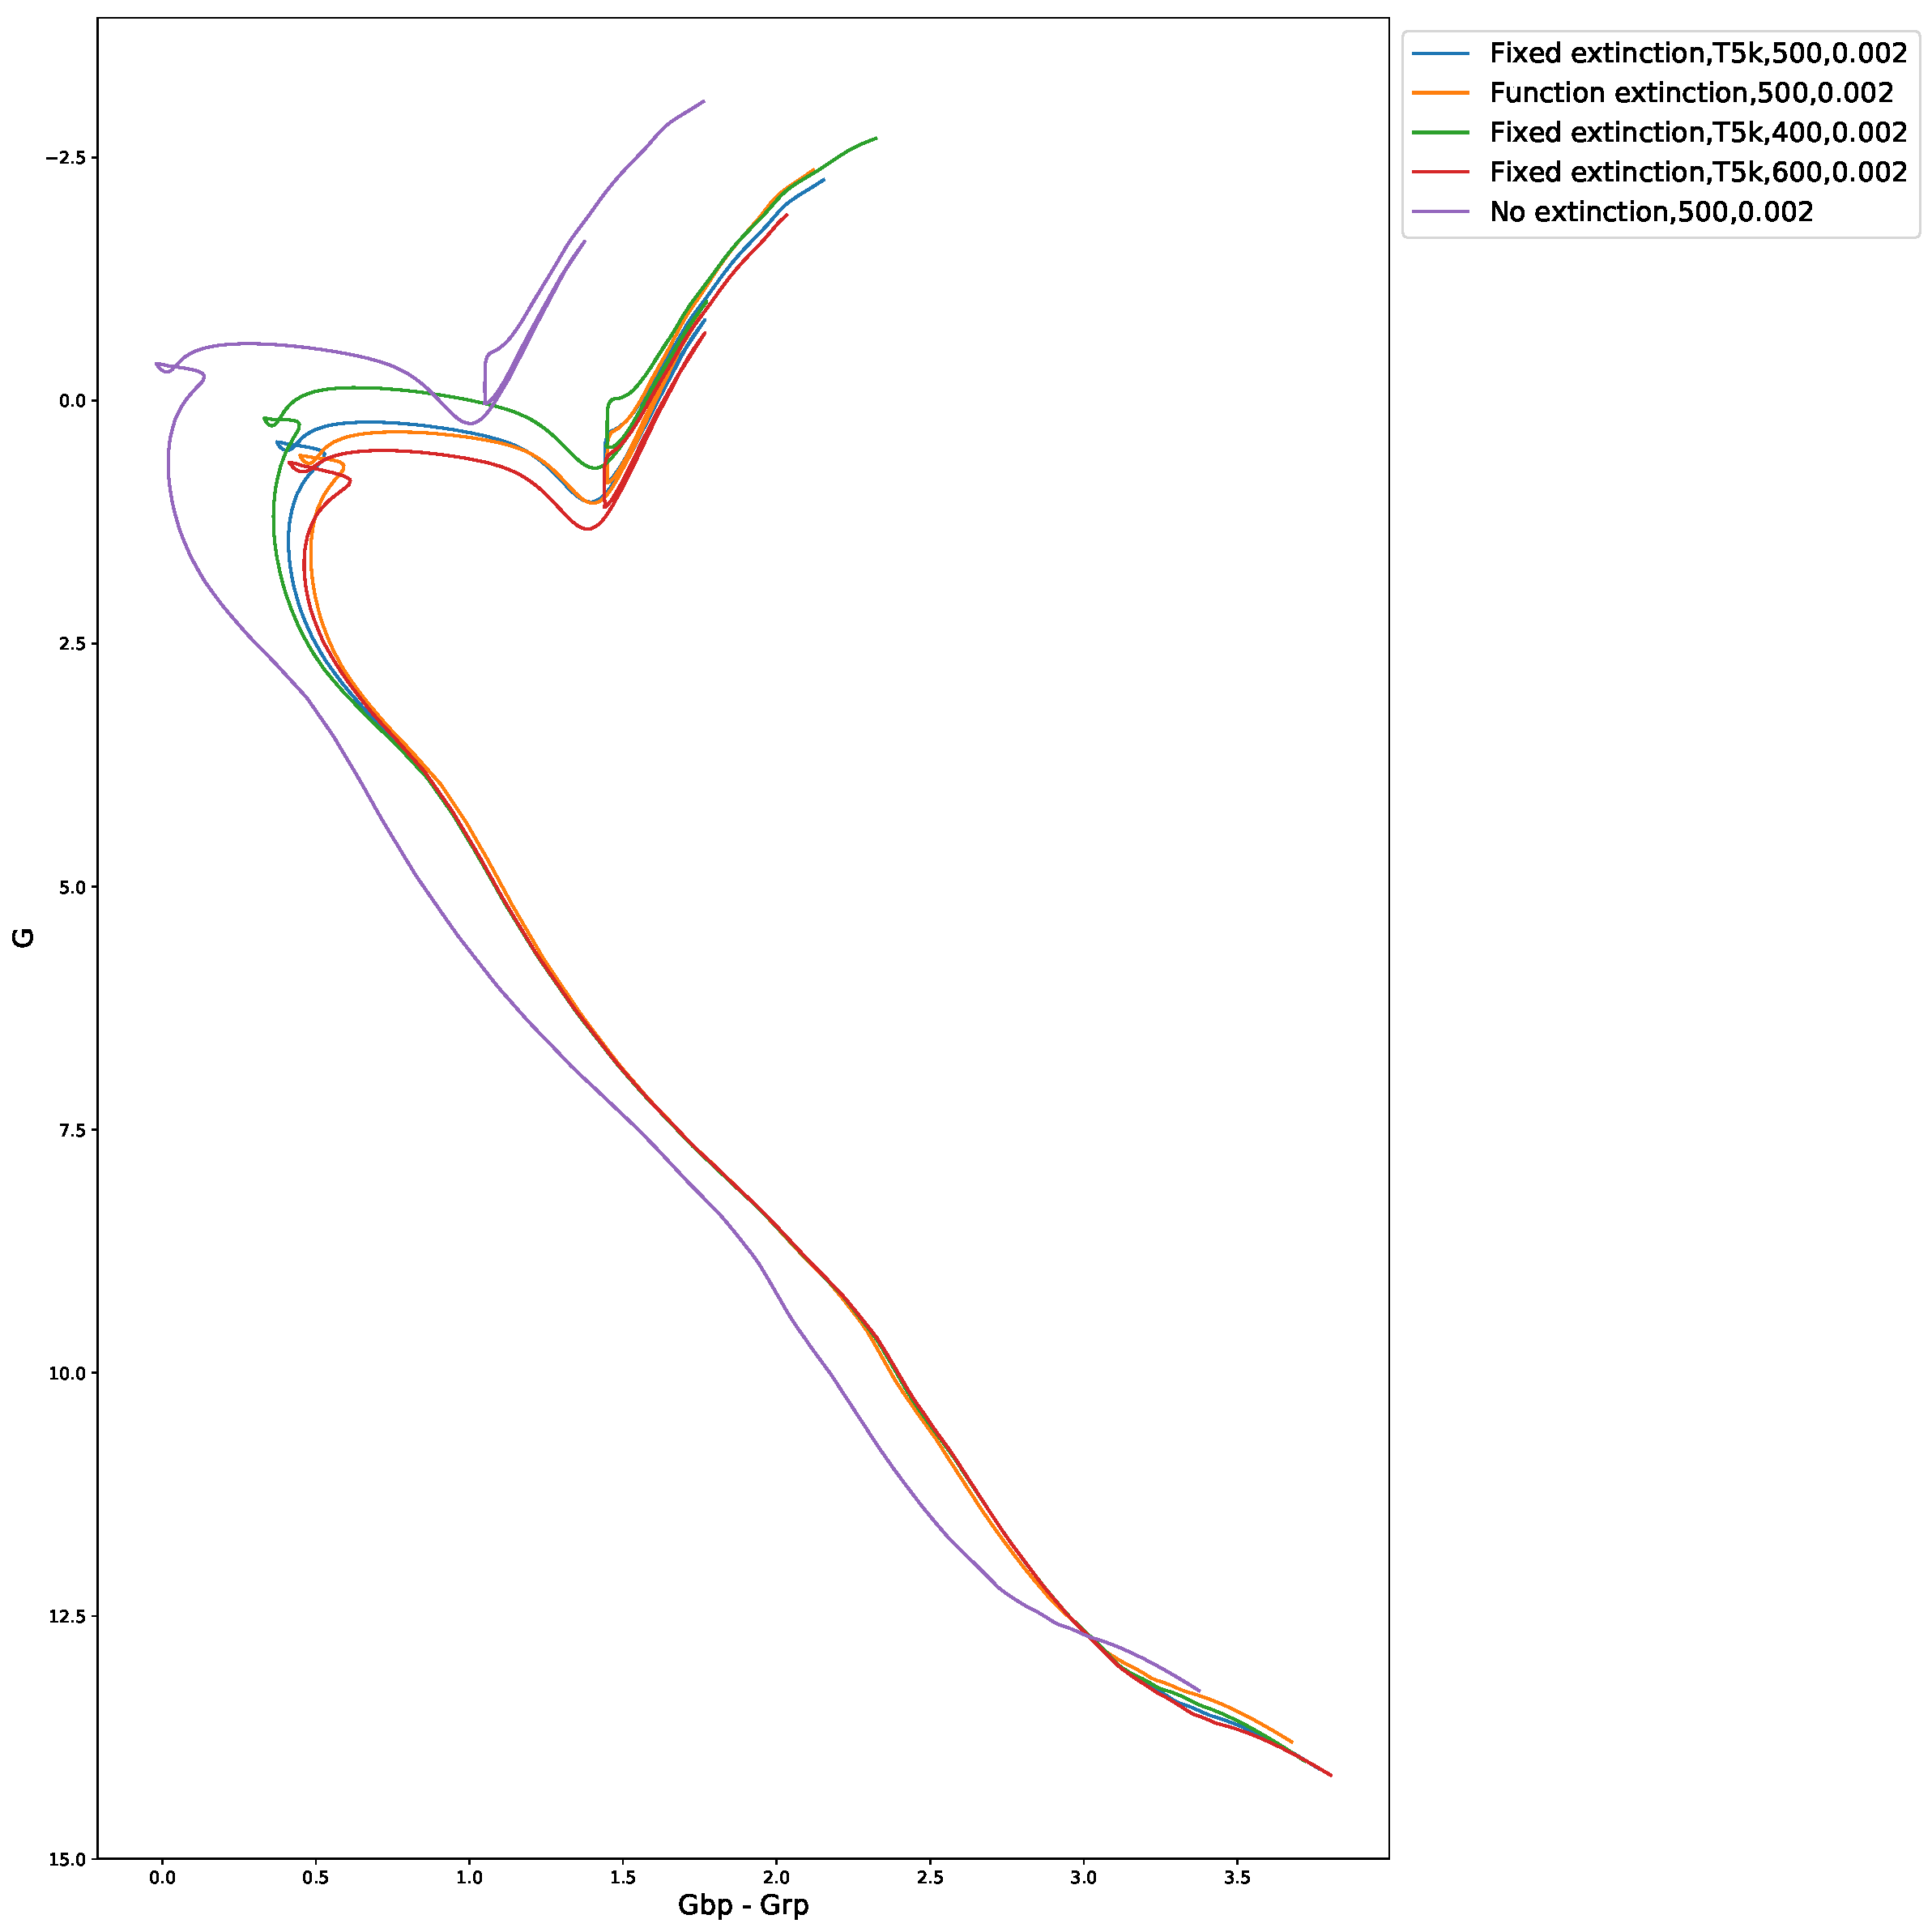
\includegraphics[width=1.0\textwidth]{../basti_isochrones_10_13Gyr/Extinction_T5k_FeH0fix_func_G_GbpmGrp_500_400_600_Myr_FeH_0p002_ref_noext_Av_1p0.pdf}
\caption{Gaia $G$-($G_{\textnormal{bp}}$-$G_{\textnormal{rp}}$) CMD with a fixed extinction coefficient equal to $(A_{X}/A_{V})_{MS}$ for each filter}
\label{gaia_isoc_T5k}
\end{center}
\end{figure}

\begin{figure}[h]
\begin{center}
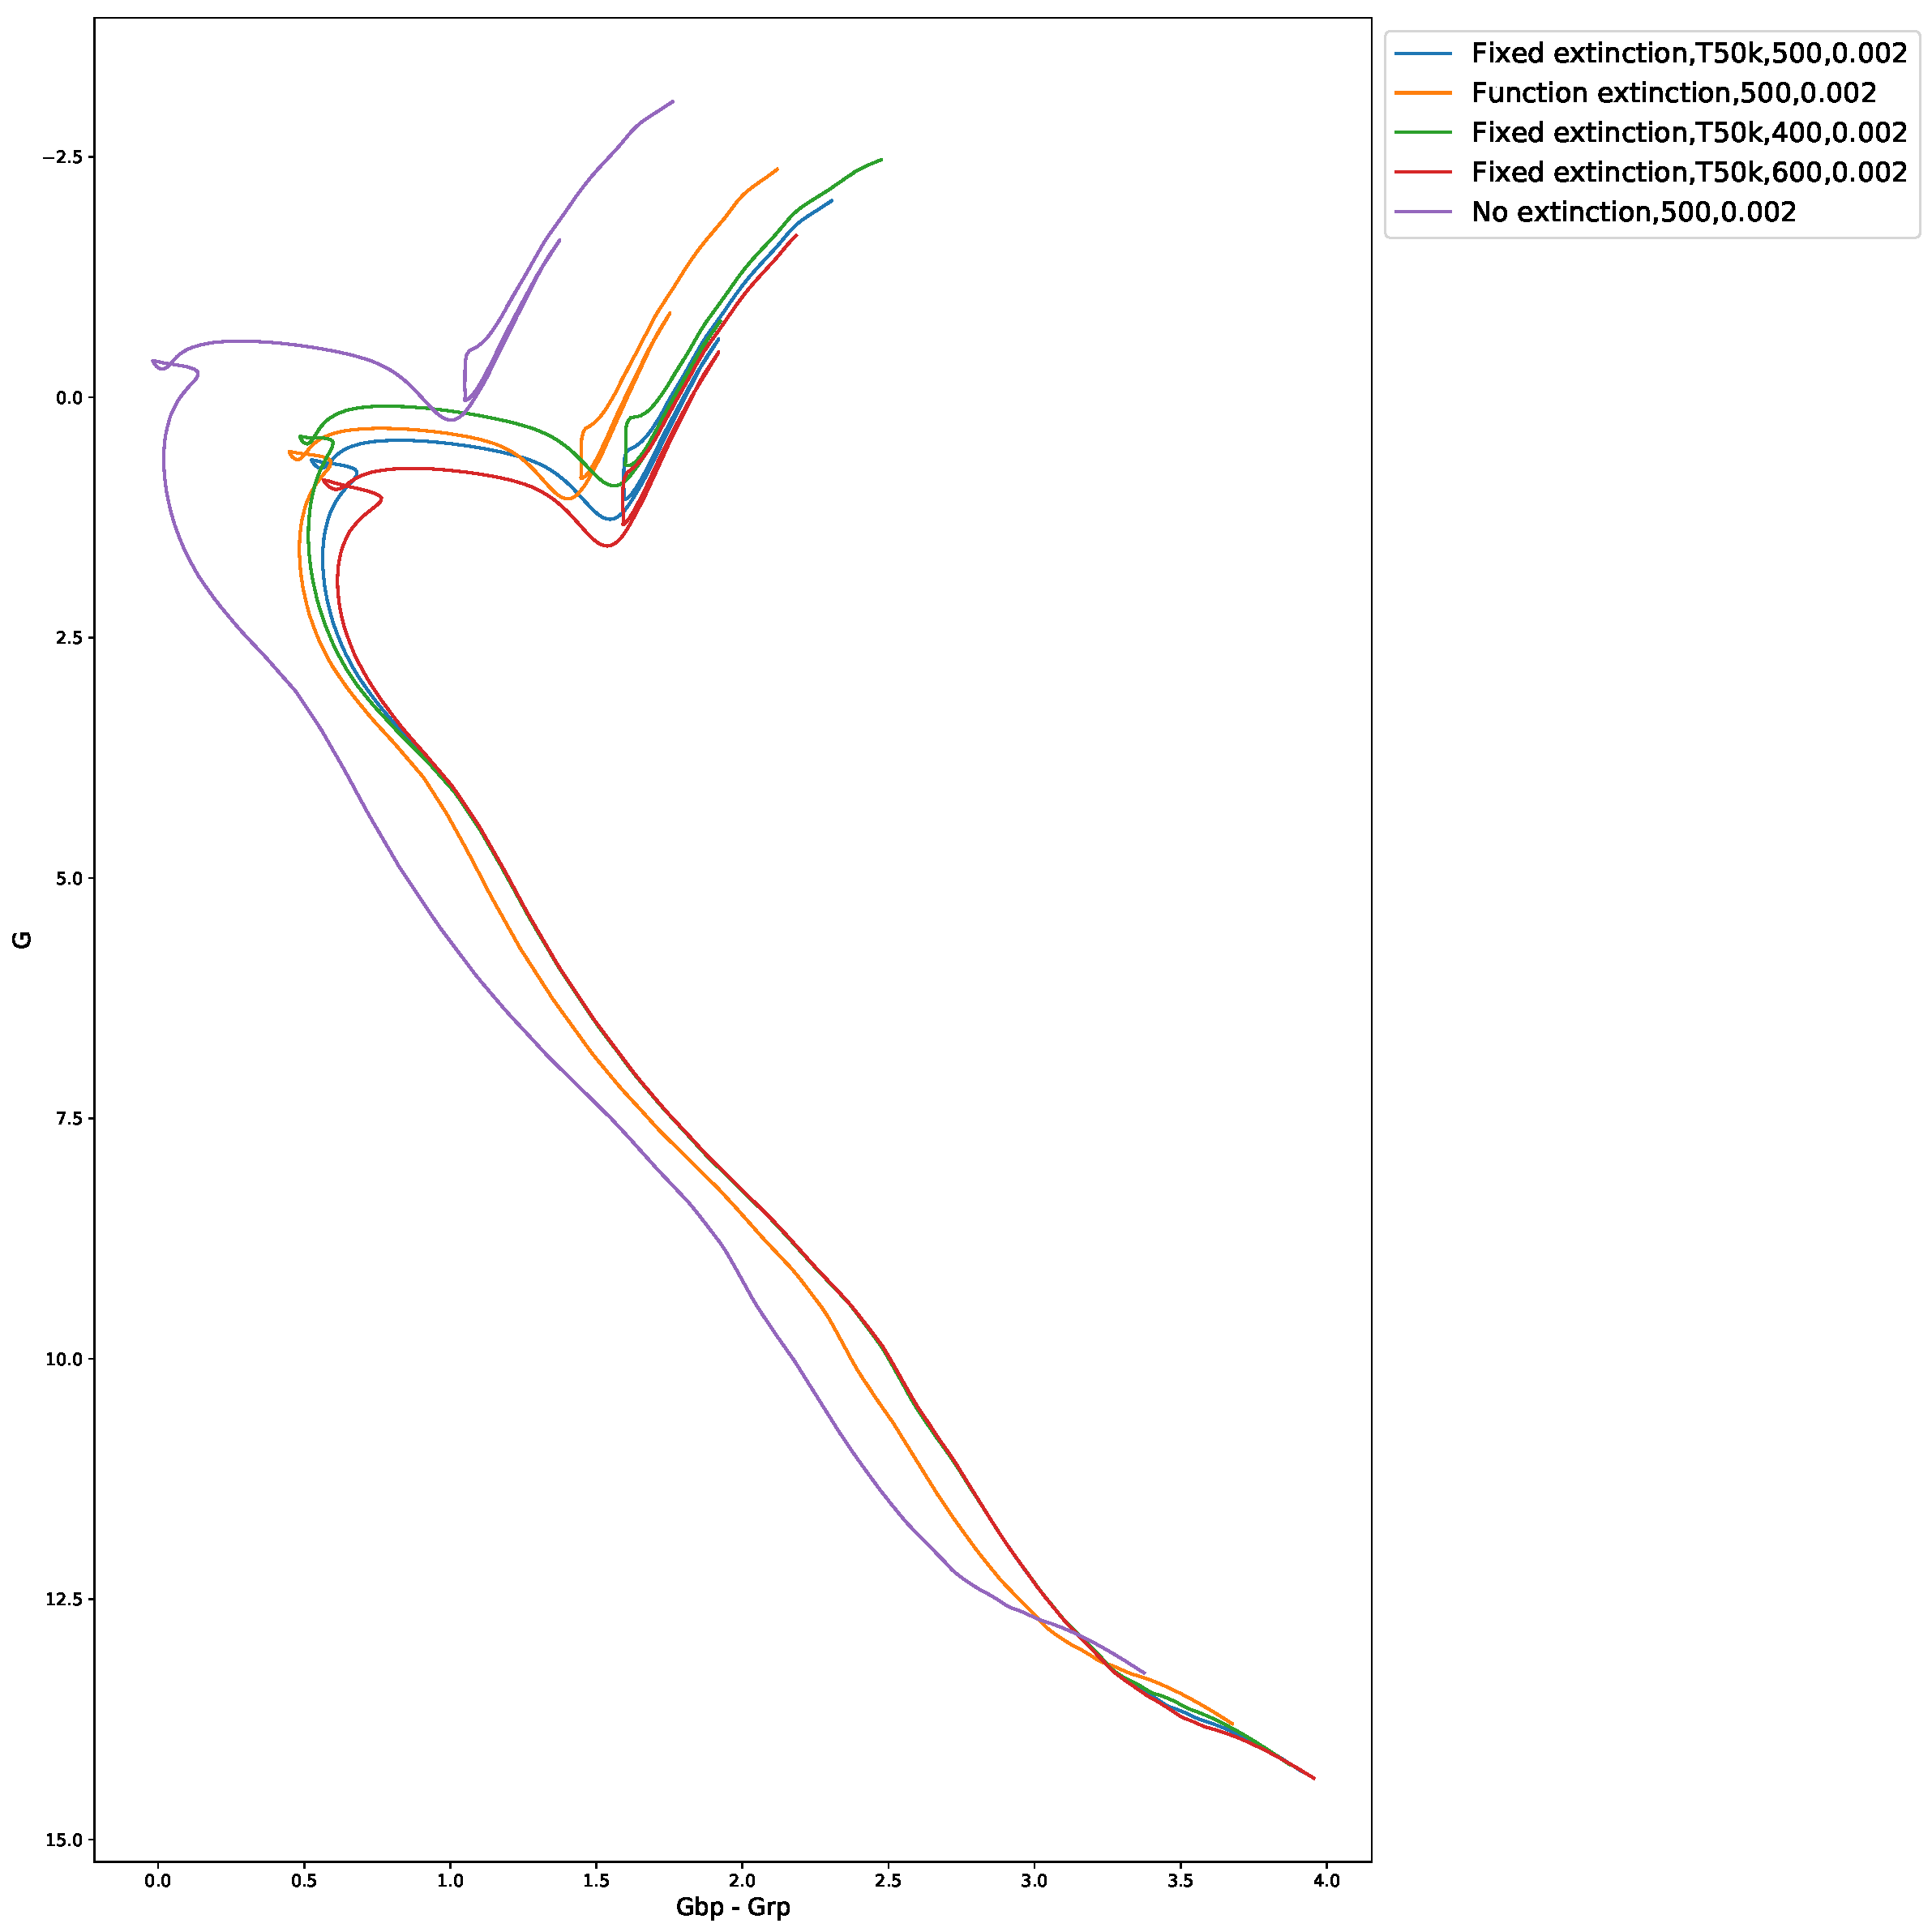
\includegraphics[width=1.0\textwidth]{../basti_isochrones_10_13Gyr/Extinction_T50k_FeH0fix_func_G_GbpmGrp_500_400_600_Myr_FeH_0p002_ref_noext_Av_1p0.pdf}
\caption{Gaia $G$-($G_{\textnormal{bp}}$-$G_{\textnormal{rp}}$) CMD with a fixed extinction coefficient equal to $(A_{X}/A_{V})_{plat}$ for each filter}
\label{gaia_isoc_T50k}
\end{center}
\end{figure}

For the Gaia CMD, when $(A_{X}/A_{V})_{MS}$ is used for the fixed-extinction isochrones, as shown in Figure \ref{gaia_isoc_T5k}, the turnoff position of the 500 Myr FBER isochrone appears to be lower on the main sequence than even the 600 Myr fixed-extinction case, suggesting that using the fixed-extinction treatment significantly and consistently over-estimates the isochrone age for an observed cluster. However, unlike the F814W-(F275W-F814W) CMD, the alignment of the main sequence continues almost along the  entire MS length. \\*

When using $(A_{X}/A_{V})_{plat}$, there is a full-isochrone position difference between the FBER isochrone and the fixed-extinction isochrones, as is seen in Figure \ref{gaia_isoc_T50k}. Since all four isochrones with added extinction in this figure assume that $A_{V} = 1.0$, alignment of the upper main sequences when using $(A_{X}/A_{V})_{plat}$ is achieved by having a lower value of $A_{V}$ for the fixed-extinction isochrones than for the function-based case. Depending on the exact value of the fixed $A_{X}/A_{V}$ used for fitting a given observed cluster, the resulting value calculated for $A_{V}$ and, subsequently, $E(B-V)$ could be significantly underestimated. \\*


\section{NGC 6793}

\begin{figure}[h!]
\begin{center}
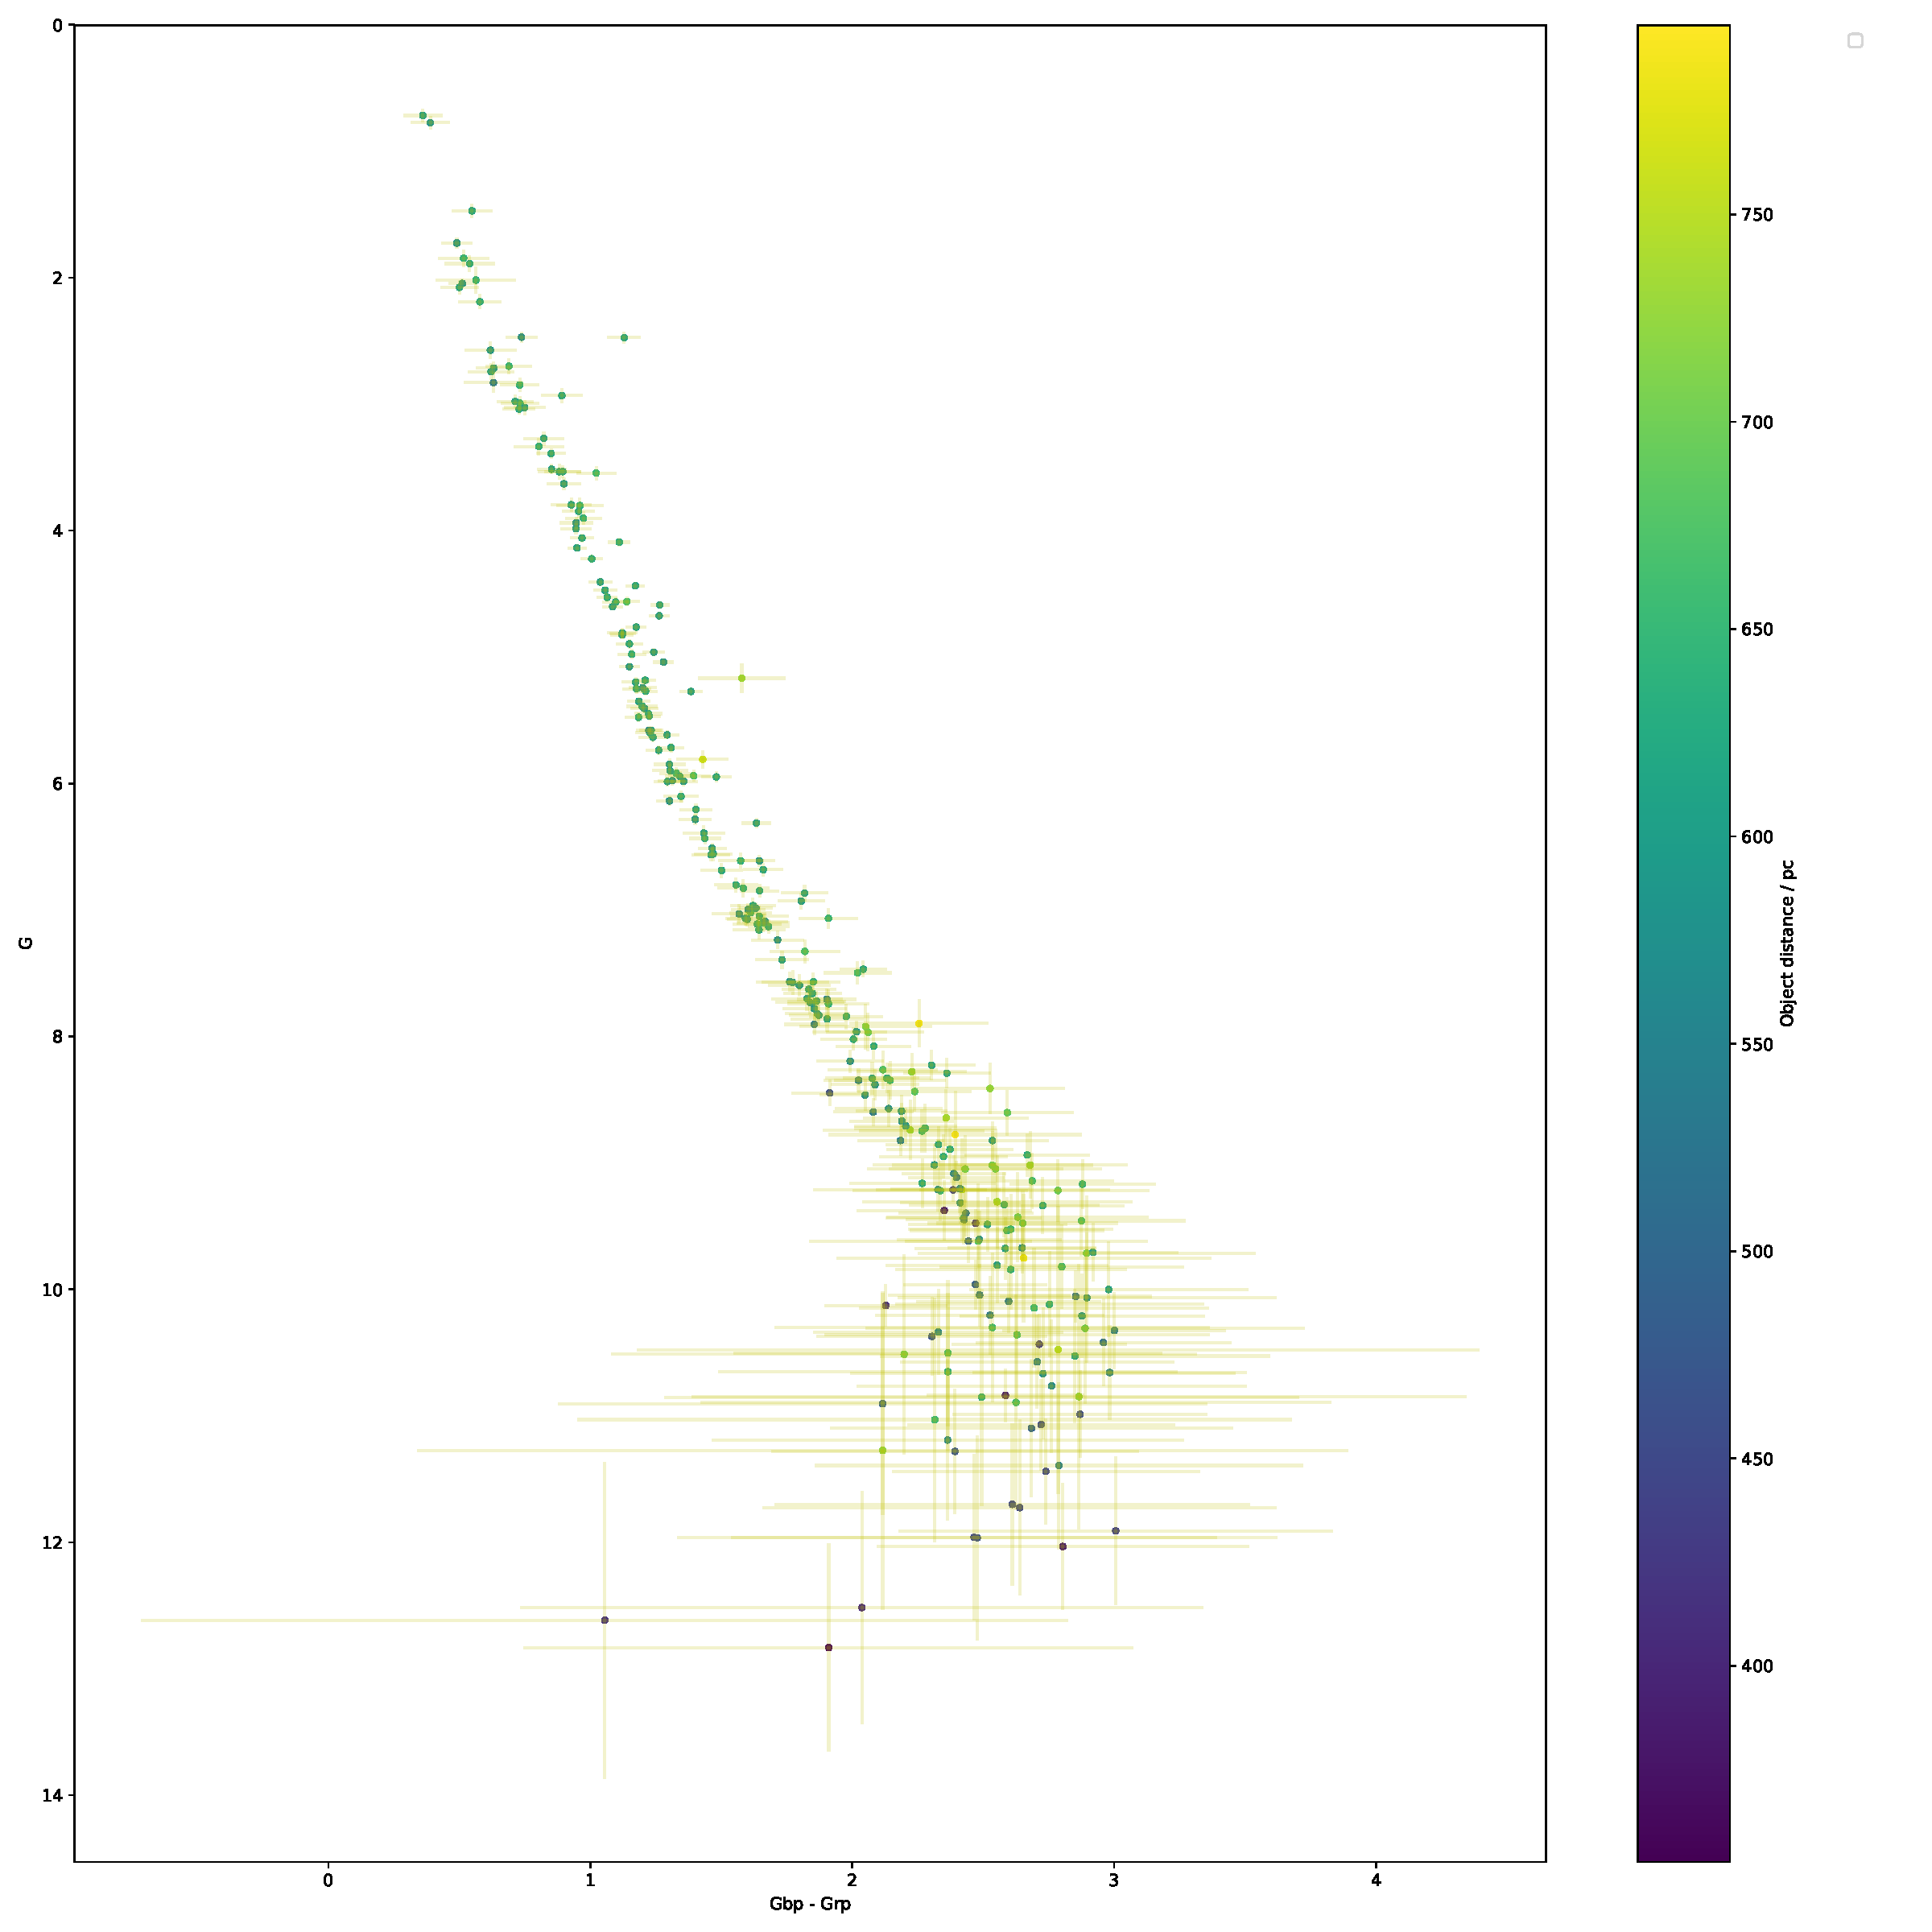
\includegraphics[width=1.0\textwidth]{../NGC_6793_CMD_observational_errorbars.pdf}
\caption{Gaia $G$-($G_{\textnormal{bp}}$-$G_{\textnormal{rp}}$) CMD showing the 274 cluster members in the final dataset, with errorbars added. The color of each object is determined by its parallax-derived distance.}
\label{NGC_6793_obs_only}
\end{center}
\end{figure}

\begin{figure}[h]
\begin{center}
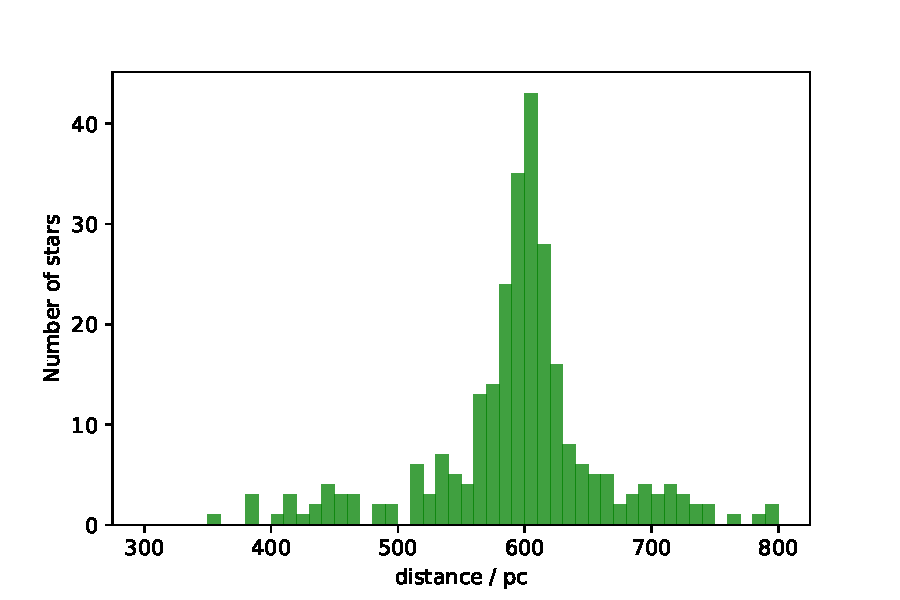
\includegraphics[width=1.0\textwidth]{../NGC_6793_distances_hist.pdf}
\caption{Histogram of distances for the 274 stars in the final observational dataset. The bins are set to a fixed width of 10 pc.}
\label{NGC_6793_dist_hist}
\end{center}
\end{figure}

The final Gaia observational sample of stars in NGC 6793 is shown as a distance-corrected CMD in Figure \ref{NGC_6793_obs_only}, with distances and photometric errors propagated directly from parallax measurements.\\*

Looking at the distances to the objects in the final sample, it is clear that there are significant variations in the observed parallaxes of individual stars, far beyond the maximum cluster radii expected for the largest open clusters, given as 16.8$\pm$2.4 pc by \cite{2006A&A...456..523S} or even radii of compact stellar associations, given as 33.2$\pm$21.7 pc in the same paper. Some objects in the original dataset (338 members in total) were even assigned negative parallax values, which are physically impossible, as a result of measurement errors. Figure \ref{NGC_6793_dist_hist} shows a histogram of the final NGC 6793 sample. It is clear that a substantial fraction of this sample have measured parallax distances which put them outside the physical limits of better-studied open clusters.\\*

However, the errors in the parallax data for objects assigned to NGC 6793 were significant, as shown in Figure \ref{NGC_6793_obs_only}, particularly for stars in the lower main sequence. This is trend is to be expected, since stars in the lower main sequence are the faintest objects in the data and therefore are the most difficult to track against background sources. The significance persists despite this project assuming that the only sources of photometric error are the parallax measurements. This leads to errors in the predicted $M_{\textnormal{ext},X}$ magnitudes, which are calculated by rearranging Equation \ref{distance_modulus}.\\*

Since the table of photometric fluxes did not include photometric errors, the parallax errors alone accounted for the total error in the calculated $M_{\textnormal{ext},X}$. Therefore, the errors on the flux measurements, calculated via error propagation, were fully independent of the absolute magnitude value of a given star. The errors on the ($G_{\textnormal{bp}}-G_{\textnormal{rp}}$) color index were calculated as standard, by adding the individual filter errors in quadrature, giving the color errors which were a factor of $\sqrt{2}$ greater than those for the individual filter fluxes.\\*

\begin{figure}[htb]
\begin{center}
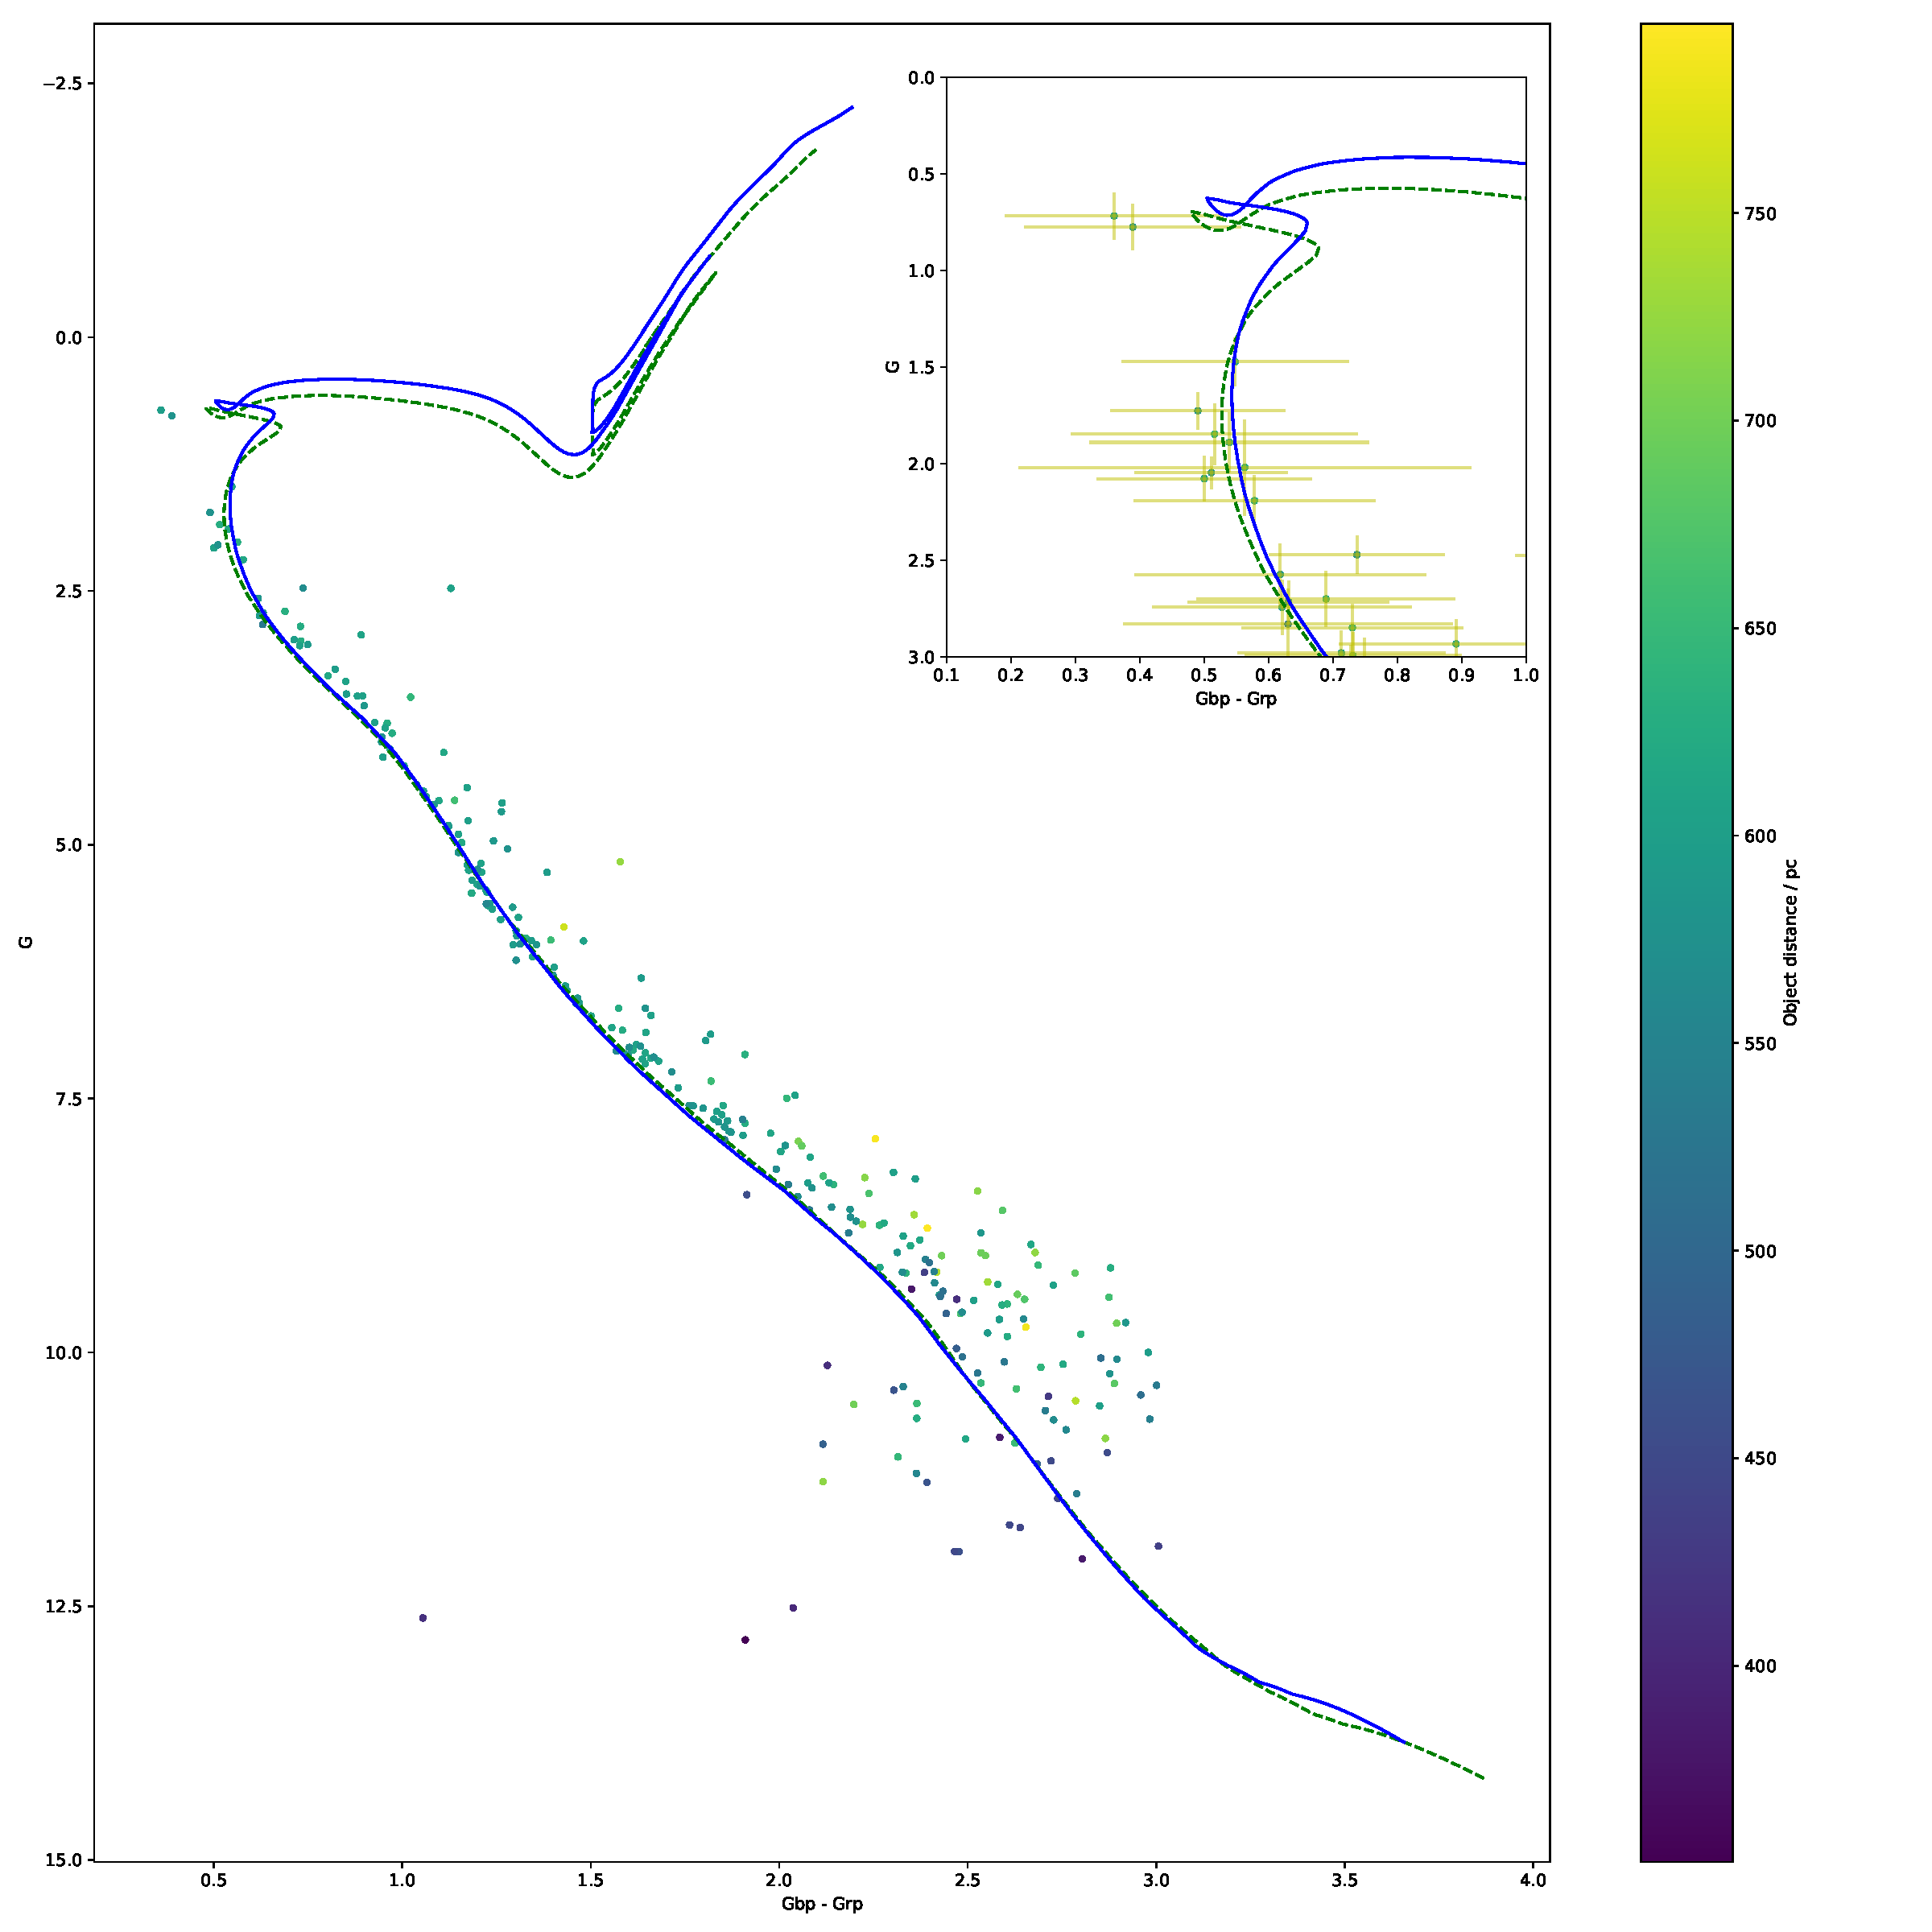
\includegraphics[width=1.0\textwidth]{../NGC_6793_CMD_FeH_0p062_Av_1p1_500Myr_all_isochrones_summary.pdf}
\caption{Gaia $G$-($G_{\textnormal{bp}}$-$G_{\textnormal{rp}}$) CMD showing the 274 cluster members in the final dataset, corrected for their individual distances with errorbars shown. The color of each object is determined by its parallax-derived distance.}
\label{NGC_6793_isoc_inset_1.1_500_0.062}
\end{center}
\end{figure}

Before comparisons with the GC18 parameters can be made, a reference isochrone, with a globally-fixed $A_{X}$ value of 0.843 and age of 600 Myr (in accordance with Table \ref{NGC6793_obs}), was made. The $A_{X}/A_{V}$ values required to achieve alignment with the upper main sequence were equal to the $(A_{X}/A_{V})_{plat}$ values for each Gaia filter. While the results from GC18 do not include a metallicity estimate for NGC 6793, it can be estimated from its age that a solar-like metallicity is likely. Therefore, the relevant isochrone has a metallicity of [Fe/H] = 0. Due to the overall red-ward shift of the isochrone caused by using $(A_{X}/A_{V})_{plat}$, as demonstrated in Figure \ref{gaia_isoc_T50k}, the GC18 parameter values are not accurate when using model functions to simulate extinction in the isochrones for NGC 6793.\\*

The alignment of the upper main sequence for a FBER treatment was achieved using a value of $A_{V} = 1.1$. The best-fit MSTO of this isochrone had an age of 500 Myr. To better align the lower main sequence, an increase in isochrone metallicity was required. The best-fit metallicity value was found to be [Fe/H] = 0.062.  However, the magnitudes of the errorbars (see Figure \ref{NGC_6793_obs_only}) dwarf any isochrone position changes due to changing extinction treatments in the main sequence. The uncertainties also render differences in position between isochrones with similar parameters insignificant, including at the MSTO, as shown in the inset plot in Figure \ref{NGC_6793_isoc_inset_1.1_500_0.062}.\\*


\begin{table}
\begin{center}
\begin{tabular}{cccc}
\hline
Cluster property & K05 & GC18 & This project \\
\hline
Age / Myr & 437 & 603 & 500 \\
$A_{V}$ / mag & 0.53 & 0.843 & 1.1 \\
$[Fe/H]$ & ? & ? & 0.062 \\
Members & ? & 271 (photometric) & 274 \\
\hline
\end{tabular}
\caption{Comparison of results from this project with observational parameters for NGC 6793 from Table \ref{NGC6793_obs}}
\label{NGC6793_result}
\end{center}
\end{table}

The wide range of distances determined for the individual stars included in the final sample, as mentioned earlier, is orders of magnitude greater than is the case for the largest better-known clusters. Stars whose distances place them furthest from the projected cluster centre make up a significant portion of the objects which are widely scattered from the expected position of the main sequence. Therefore, between this and the magnitude of the errorbars in the lower main sequence in particular, the isochrone fits shown in Figure \ref{NGC_6793_isoc_inset_1.1_500_0.062} can be considered accurate. \\*

A potential source of uncertainty when comparing the best-fit isochrone results of this project for NGC 6793 with those from GC18 comes from the fact that this project employs the latest BaSTI isochrone database \citep{2018ApJ...856..125H}, while GC18 uses the PARSEC isochrone database \citep{2017ApJ...835...77M}. The use of different isochrone software could impact the validity of comparing the $A_{V}$ values, ages and metallicities arising from both extinction treatments.\\*

\cite{2019MNRAS.483.4949G} carried out a detailed set of observations of the Galactic globular cluster NGC 5904 in 29 photometric bands. The CMDs created from this data were used to fit isochrones from five different databases, including PARSEC and BaSTI. They adopted the \cite{1989ApJ...345..245C} extinction law with the parameters having values of $R_{V} = 3.60\pm0.05$ and $A_{V} = 0.20\pm0.02$. As shown in Table \ref{NGC5904_obs_gontcharov}, the Gaia colour excess $E(G_{\textnormal{bp}} - G_{\textnormal{rp}})$ for NGC 5904 differs significantly between the best-fits from the two databases, which in turn causes disagreements for the projected cluster age and (photometric) distance. Across all filter systems and isochrone databases, the authors calculated mean estimates of the cluster properties and found that the resulting photometric distance to be in agreement with the cluster distance calculated from the Gaia parallaxes of the cluster members.\\*

\begin{table}
\begin{center}
\begin{tabular}{ccc}
\hline
Cluster property & PARSEC & BaSTI \\
\hline
$E(G_{\textnormal{bp}} - G_{\textnormal{bp}})$ / mag & 0.080$\pm$0.02 & 0.013$\pm$0.03 \\
Age / Gyr & 11.5 & 12.5 \\
Distance / pc & 7600 & 8400 \\
\hline
\end{tabular}
\caption{Comparison of best-fit parameter results for NGC 5904 using PARSEC and BaSTI. Data taken from \cite{2019MNRAS.483.4949G}.}
\label{NGC5904_obs_gontcharov}
\end{center}
\end{table}

In the case of the analysis of NGC 6793 made here, the distance measurements are derived from parallax measurements and so are unaffected by the choice of isochrone software, allowing the GC18 cluster distance to be validly assumed here (as 600 pc to the cluster centre). Furthermore, using the PARSEC-derived parameters from GC18, an accurate BaSTI model isochrone was produced successfully, without any deviation from standard assumptions made for an extinction model with a globally-constant value of $A_{X}/A_{V}$. Therefore, it was concluded that the validity of comparing of the respective $A_{X}$, [Fe/H] and age values from GC18 and this project was not endangered by the use of different isochrone databases by each study.\\*

As predicted by the comparisons made in Section \ref{Gaia_isoc}, the isochrone with a function-based extinction at the GC18 estimated value of $A_{V} = 0.843$ is systematically too blue and too bright to fit to the observed CMD of NGC 6793. This remains the case regardless of changes in age and metallicity. Therefore, as predicted, there is significant disagreement between the $A_{V}$ values between the two extinction-calculation methods.

There are considerable uncertainties for the parameters in both isochrones in Figure \ref{NGC_6793_isoc_inset_1.1_500_0.062}. Most fundamentally, the position of the MSTO is reliant only on the position of the four brightest cluster members, of which the brightest two, if the isochrones are accurate, appear to be part of part of the cluster's SGB hook. The objects' parallax errors, as shown in the inset of Figure \ref{NGC_6793_isoc_inset_1.1_500_0.062}, are large enough to make any disagreement with either of the isochrones insignificant, even with substantial changes in metallicity. Any changes in $A_{V}$ and age cause misalignment with the main sequence and MSTO, respectively, making analysis of their impact on the SGB hook region unnecessary.\\*

\chapter{Conclusion \& future work}
In all cases, applying a fixed extinction to all points in an isochrone causes the main-sequence turn-off to occur at a more luminous, bluer point in a given CMD than the MSTO point for an isochrone with extinction values for every star described using an function fitted to empirically-derived data for each filter.\\*

The significance of this position change is dependent on the filters used to construct the particular CMD in question. The position changes in two of the four CMDs studied are insignificant.\\*

The WFC3 F814W-(F275W-F814W) CMD shows significant differences between the positions of certain sections isochrones treated under different extinction-calculation approaches, particularly for the lower main sequence but also affecting for the MSTO, depending on the value of $A_{X}$ used in the fixed-extinction case. This is a consequence of the much larger variation of extinction between different stellar types at shorter wavelengths, in this case in the UV.\\*

The Gaia photometric CMD is highly sensitive to the $A_{X}$ values applied to the filters. This applies not only when comparing the fixed-$A_{X}/A_{V}$ approach to the function approach, but also when comparing the fixed approaches using $(A_{X}/A_{V})_{plat}$ and $(A_{X}/A_{V})_{MS}$. This underscores the substantial risk of incorrect assumptions being made when fitting isochrones to observational data with a single globally-fixed $A_{X}$ value across all stellar models, which in turn leads to incorrect estimates of important cluster parameters.

\section{Future work}
There are multiple ways to extend the applicability of the work done in this project. The most obvious example is both to study more CMDs in the filter systems used in this project acquire and to utilise the response functions of more filter systems, particularly for more modern and more sensitive instruments, such as the James Webb Space Telescope (JWST) and the proposed WFIRST and PLATO space telescopes, to create extinction-ratio models for observations made with these instruments.\\*

Another extension would be to apply the FBER approach to observed clusters with isochrone ages determined using the globally-fixed $A_{X}$ approach. If, as predicted for the limited examples studied in this project, the isochrone ages of a given cluster CMD are greater when employing a fixed-extinction approach, there is the possibility of a systematic decrease in the predicted ages of these observed after comparison with ages derived using a function-based approach.\\*

Regarding the case of NGC 6793, follow-up observations with Johnson-Cousins filters, if feasible, could resolve the $A_{V}$ disagreement between extinction-calculation methods by providing a direct measured value upon which the Gaia extinction ratios can be calculated.\\*

Finally, the limits on the accuracy of the model functions presented here require investigation, particularly the accuracy limit at the lowest $T_{\textnormal{eff}}$ values available from ATLAS9. This could be done using the same approach as that used by \cite{2008PASP..120..583G}, who use models from other sources to extend their bolometric correction database to a minimum $T_{\textnormal{eff}}$ of ~ 1000 K. The coolest known stellar objects (excluding brown dwarfs) have $T_{\textnormal{eff}} \gtrsim 2500$ K. Extending the dataset would constrain the allowed behaviour of the model functions in the lowest ATLAS9 metallicities. Currently, the lack of data below 3500 K prevents investigation of the significance of the tail-flick phenomenon, since the phenomenon, at present, extends to (and possibly beyond) the lower-$T_{\textnormal{eff}}$ limit for the affected filters.

%\bibliographystyle{ieeetr}
\bibliographystyle{mnras} % unsrtnat
\bibliography{mphil_thesis}

\end{document}